Final video
\url{https://www.youtube.com/watch?v=UsDRPjDwr8A}
screenshots

%=========================================================================================================

\subsection{Case Study - St Salvator's Chapel}
Founded in 1450 but internally stripped of its medieval fittings during the Protestant Reformation (1517 - 1648), St Salvator's chapel in St Andrews looks markedly different in the present day than it did upon its completion. An existing VR reconstruction of the chapel as it stood in the period 1450-1460 \& the marked differences between the internal appearance of the VR building \& the current building (including the replacement of the original stone roof with a wooden one \& drastically different dividing of the internal space) make this chapel an ideal candidate within the context of cultural heritage for a mobile XR system to be applied. Figure \ref{sallies_layout} shows the 1450-1460 layout of the chapel (including the paths that the IPS has been prepared upon).

\begin{figure}[h]
	\begin{center}
		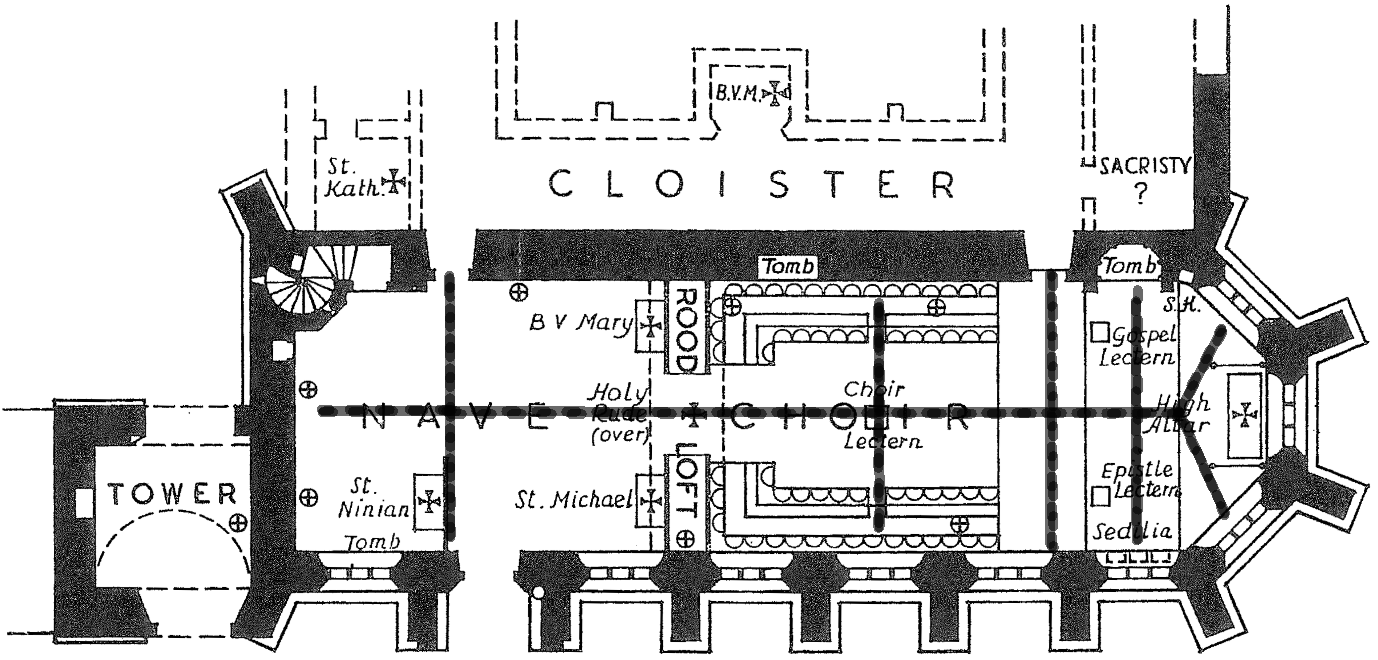
\includegraphics[width=0.7\textwidth]{sallies_layout.png}
		\caption{Floor plan of St Salvator's chapel, with IPS routes.}
		\label{sallies_layout}
	\end{center}
\end{figure}

%=========================================================================================================

\section{Investigation 1 - The Case for Mobile XR}
\label{investigation1}
This first investigation will compare interaction with the RW \& VR chapel using Mirrorshades to interaction with the same content separately, the latter being the approach usually adopted for dissemination of VR content in cultural heritage contexts. Participants will complete a task that will promote active comparison \& contrast of the RW \& VR environments, whilst navigating a set route. This investigation will gauge through experimentation whether the Mirrorshades platform provides any value over the traditional manner in which the same VR content might be disseminated at a cultural heritage site.

%spatial \& temporal separation

\subsection{Setting \& Task}
This investigation comprises two phases;

\begin{enumerate}
	\item Participants will experience the RW \& VR chapels separately. They will navigate the VR chapel from a stationary position, as one might expect to see a VR installation at a cultural heritage site, using the Xbox controller to move around the VR environment observed via the HMD. The HMD will obscure their view of the RW chapel around them. Subsequently, they will navigate the RW chapel without the HMD or any associated equipment.
	\item Participants will experience the RW \& VR chapels in tandem using the Mirrorshades platform. They will wear the HMD, holding the Xbox controller in their right hand \& the smartphone in their left, with the laptop \& battery pack in a satchel worn over one shoulder. One style of transition will be available to the participants during this phase.
\end{enumerate}

In all 3 scenarios (phase 1 VR, phase 1 RW, phase 2 RW + VR) the participant will navigate the same route \& will be instructed to identify a particular feature/object within the chapel (see figures \ref{pews} \& \ref{ceiling}), situated somewhere upon the set route, that differs in its appearance \&/or location between the RW \& VR chapels. The order in which the two phases are completed will be randomised between participants, as will the features that they are told to observe in each phase. Participants will have a maximum length of time to navigate the route \& will be allowed to stop before this time has elapsed should they wish.

%\begin{figure}[h]
%	\begin{center}
%		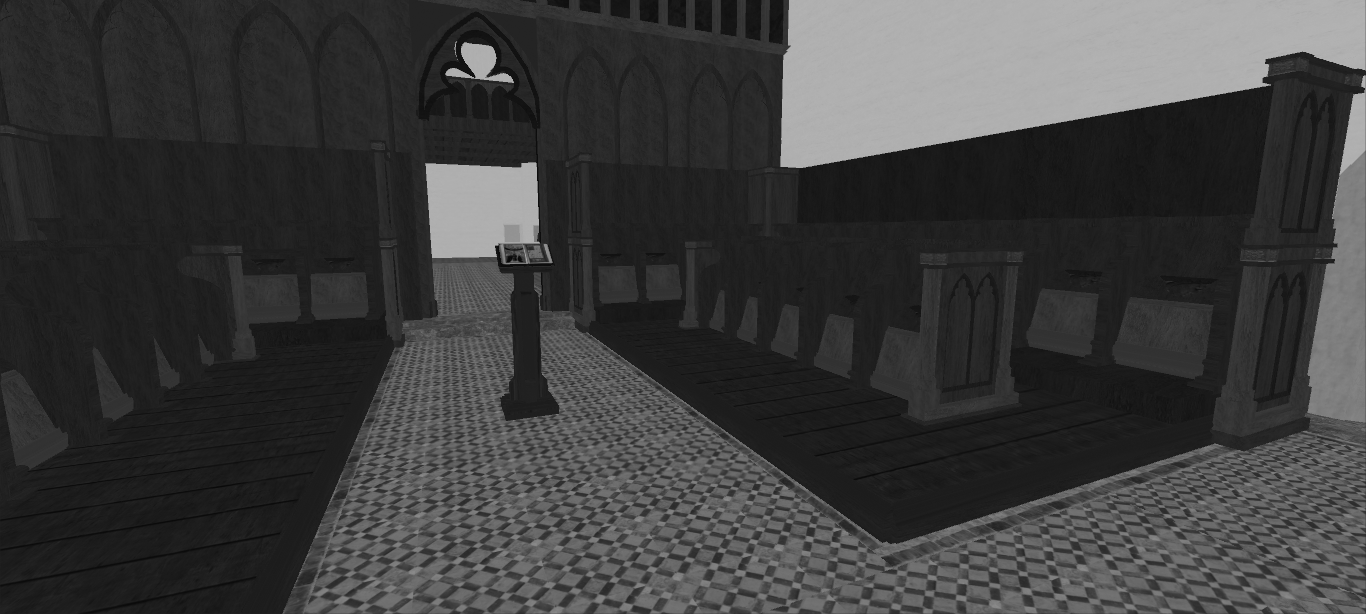
\includegraphics[width=0.7\textwidth]{pews.png}
%		\caption{Chapel pews, greater in number in present day.}
%		\label{pews}
%	\end{center}	
%\end{figure}

%\begin{figure}[h]
%	\begin{center}
%		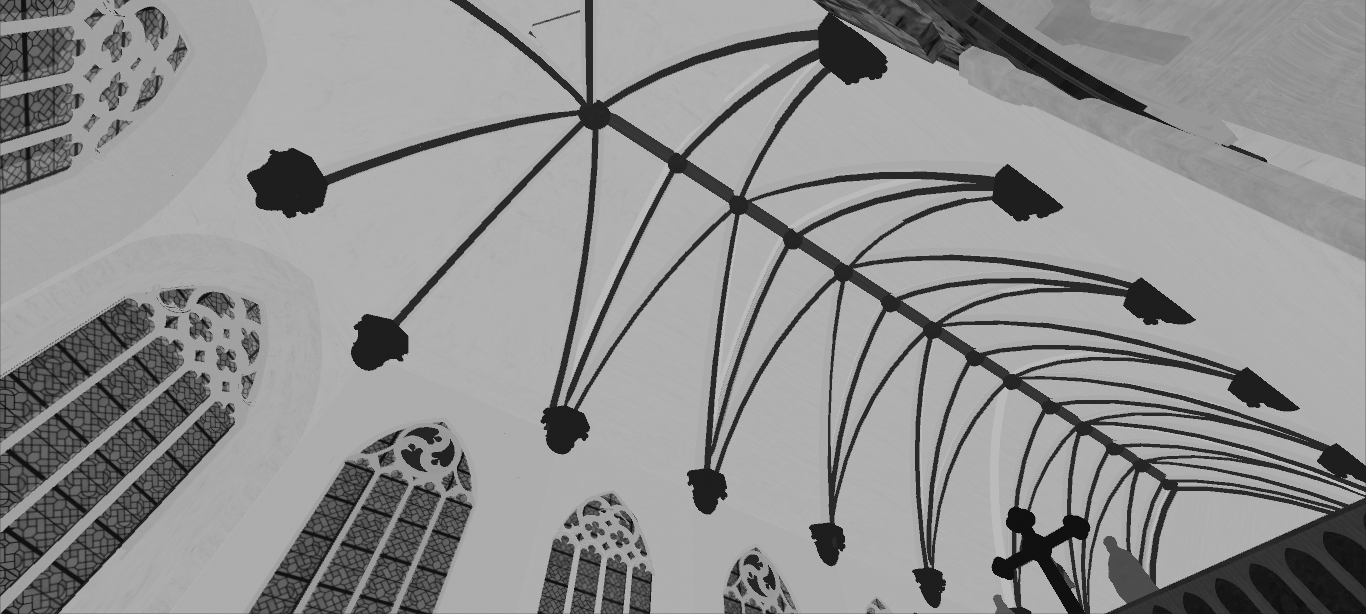
\includegraphics[width=0.7\textwidth]{ceiling.png}
%		\caption{Chapel ceiling, different construction in present day.}
%		\label{ceiling}
%	\end{center}	
%\end{figure}

%\begin{figure}[h]
%	\begin{center}
%		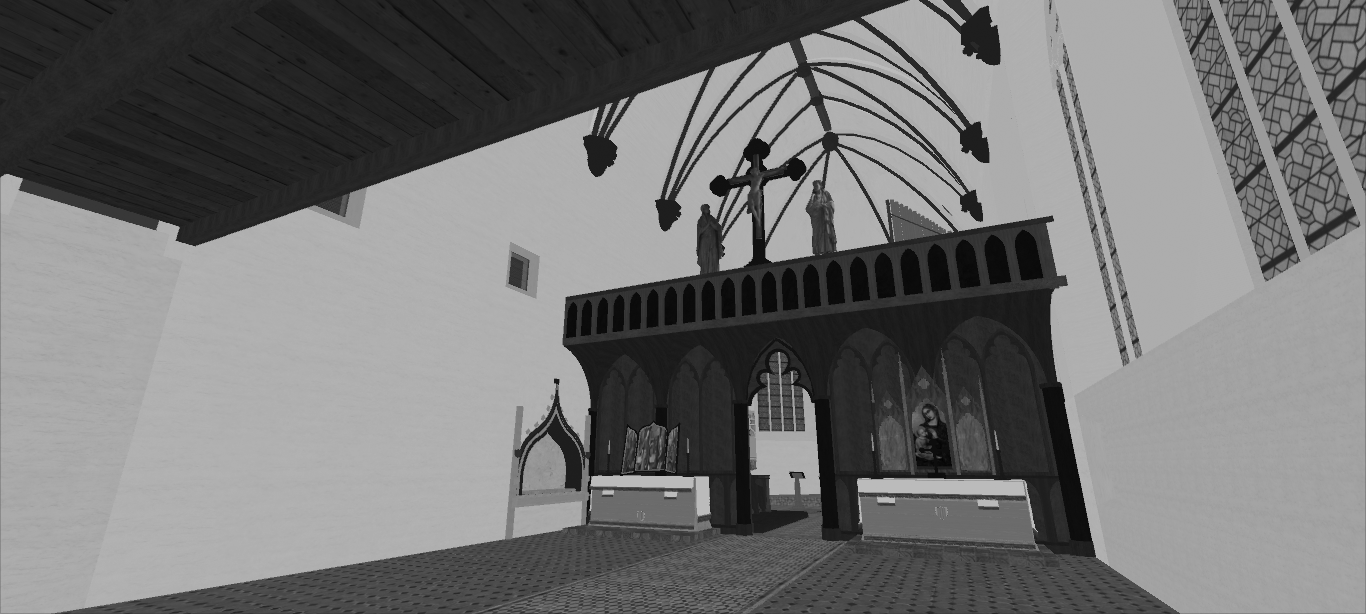
\includegraphics[width=0.7\textwidth]{division.png}
%		\caption{Division of the internal space of the chapel, different position in present day.}
%		\label{division}
%	\end{center}	
%\end{figure}

%rows/number of pews
%position of dividing wall
%colour/construction of ceiling
%number/position of lecterns

\subsection{Evaluation Techniques}
Evaluation will be performed via a short structured interview \& completion of the System Usability Scale (SUS)~\cite{Brooke1996}.

%\begin{itemize}
%	\item (General) Which did you prefer?
%	\item Which did you think made it easier for you to perform comparisons between real \& virtual?
%	\item Which was more rewarding (if you were visiting the site genuinely)?
%	\item Which gave a better understanding of the changes that have been effected to the building?
%	\item Did you notice/discover anything in one scenario that you didn't in the other?
%	\item Etc.
%\end{itemize}

\subsection{Hypothesis}
SUS responses are expected to average fairly low due to the cumbersome nature of the platform's implementation. Participants who are able to overcome this cumbersomeness are expected to respond favourably to the platform, with those who cannot overcome it responding in favour of the traditional `separate' approach instead.


\subsection{Experimental Task \& Setting}
For these experiments, the HMD is worn upon the head of the participant \& is connected to the laptop computer, battery pack \& wireless receiver worn in a satchel. The smartphone is held in the left hand \& the Xbox controller is held in the right hand (all of the buttons \& triggers used for these experiments are on the right hand side of the controller, designed to be activated with only the right hand).

A task similar to that employed in the first investigation (see section \ref{investigation1} will be employed, encouraging participants to encounter multiple different scenarios of moving, remaining stationary, etc.

\subsection{Evaluation}
%*** explain why we need both Quantitative & Qualitative data?

%What transition styles are preferred in what situations?
%What affects which transition styles are preferred (eg what are the 'situations')?

Evaluating users' preferences toward different methods of transitioning between visual stimuli in different situations pertains to studying their reactions \& responses to ascertain the effect upon their focus of attention, concepts which are largely psychological in nature \& highly subjective~\cite{Ijsselsteijn2001}. Thus, subjective measures will produce the bulk of the data for evaluation. However, objective data will also be collected \& cross referenced with the subjective data in attempts to support or contradict any relationships that are identified.

It is hypothesized that a manner of transitioning between visual stimuli which results in a less severe BIP will be preferable to a manner of transitioning which results in a worse BIP. As focus in the Waterworth model is most closely related to presence in the VR literature~\cite{Waterworth2001}, one of the subjective measures that will be used in this evaluation will be an established presence measure, to try to capture the behaviour of the user's position upon the focus axis.

\subsubsection{Subjective Quantitative - Post-Task Questionnaire}
After completing the task, participants will respond to the Igroup Presence Questionnaire (IPQ)~\cite{Schubert2001} (see appendix \ref{ipqitems} for the items of the IPQ) which will provide subjective quantitative insight into their experiences with the system, in particular in relation to their position upon the focus axis of the combined model. The IPQ represents a useful questionnaire for evaluation of users' subjective experiences of using the Mirrorshades platform because its terms, especially in the `spatial involvement' scale, question about the RW environment in a manner that does not explicitly present it as a `distraction' from the VR interaction as many other presence questionnaires do.
%examples of other presence questionnaires that present RW stimuli as 'distractions'?

%citation for the components being independent
%The IPQ consists of one general item (G), five items in the `spatial presence' (SP) scale, four items in the `involvement' scale (INV) \& four items in the `realness' scale (REAL). For the purposes of this study, all of the REAL items save REAL2 will be omitted from the questionnaire. The REAL items are primarily concerned with eliciting how `real' participants considered the virtual environment to be. These questions are useful for traditional VR experiences where the user is encouraged to suspend belief \& believe the VR environment they are perceiving to be `real' (the same experiences for which RW stimuli are usually considered a `distraction'). The Mirrorshades platform, however, is less concerned with convincing participants that a VR environment is real \& is more concerned with the juxtaposition of VR \& RW environments.
%It is believed that the other REAL questions will get the participants thinking about the wrong things & hamper their responses when talking about XR

%hypothesis
Whilst a traditional VR experience would hope to elicit high SP1 \& SP4 results combined with low INV1 \& INV3 results, Mirrorshades participants are expected to report high SP1 \& SP4 combined with \textit{high} INV1 \& INV3. The results from participants in this investigation will be compared against those who partook in a `traditional' VR experience wherein RW stimuli were considered a distraction.

% *** But what about the factor analysis, what effect does removing the REAL component have on that?

\subsubsection{Subjective Qualitative - Interview}
A structured interview will be performed after the IPQ has been completed.

\subsubsection{Objective Quantitative - Automatic Data Logging}
The Unity app logs the following quantitative data each frame to a tab separated variable (\texttt{.tsv}) file;

\begin{itemize}
	\item \texttt{<frame number>}
	\item \texttt{<timestamp>} - according to the laptop's internal clock
	\item \texttt{<original\_position>} - the position as a Unity \texttt{Vector3} where the user begins the experiment
	\item \texttt{<position>} - the position as a Unity \texttt{Vector3} where the user is on this frame
	\item \texttt{<delta\_x>} \& \texttt{<delta\_z>} - the difference in the \texttt{x} \& \texttt{z} axes between \texttt{<original\_position>} \& \texttt{<position>} on this frame
	\item \texttt{<left\_rotation>} \& \texttt{<right\_rotation>} - the orientations as Unity \texttt{Quaternion} of the two Unity camera game objects
	\item \texttt{<base\_oapcity>} - the maximum opacity of the game objects upon which the webcam feeds are rendered (see section \ref{subsub-baseopacity})
	\item \texttt{<left\_opacity>} \& \texttt{<right\_opacity>} - the opacity on this frame of the game objects upon which the webcam feeds are rendered
	\item \texttt{<auto\_tick>} - whether a periodic switch is in progress (see section \ref{subsub-periodic})
	\item \texttt{<auto\_duration>} \& \texttt{<auto\_spacing>} - the interval \& duration values of the periodic hard switching
	\item \texttt{<framerate>} - an estimate of the current frame rate (frames per second)
	\item \texttt{<A\_button>}, \texttt{<B\_button>} \& \texttt{<right\_trigger>} - the current values of these inputs on the controller
\end{itemize}

\vspace{4mm}

An example line of this output;

\begin{center}
	\texttt{420	08-05-2014 12-34-36-257	(3.4, 1.0, -8.3)	(0.3, 1.0, -8.3)	3.153522	0.0001955032	(-0.1, -0.7, -0.1, 0.7)	(-0.1, -0.7, -0.1, 0.7)	1	1	1	False	0	0	39.57977	False	False	0}
\end{center}

These data are expected to reveal relationships between various different metrics \& the choice of transition methods. For example, it is expected that participants will perform short transitions to VR or transitions to a mix of RW \& VR when moving \& perform longer transitions to VR when stationary. This kind of relationship will support or contradict the subjective data collected through questionnaire \& interview.

%*** SUS?

\subsubsection{Objective Qualitative - Video Recording}
%*** talk about not prompting them with 'think aloud' vs prompting (where prompting changes their responses)
During experiments, the video feed being displayed by the HMD will be recorded \& the user will be recorded using a video camera (both video \& audio). The video of the HMD graphics will be used in comparison with the quantitative data, while the video \& audio recording of the user will provide objective insight into their behaviour.

%\subsection{Evaluation Techniques}
%These data will make it possible both to statistically assess preferred switching/fading methods, but also to infer any relationships between different switching/fading methods \& other behaviours: for example, a certain style of switching/fading may frequently appear after a period of movement, but rarely when the participant is stationary.

%\section{Hypothesis}
%Null hypothesis includes things like;
%\begin{itemize}
%	\item different transitions do not alter user `enjoyment'
%	\item users will not prefer one transition over another
%	\item choice of transition will have no effect on circumstances/scenarios
%	\item users will not move head less when walking
%	\item users will not spend less time in virtual when walking
%	\item etc.
%\end{itemize}

%=========================================================================================================

\begin{figure}[h]
	\begin{center}
		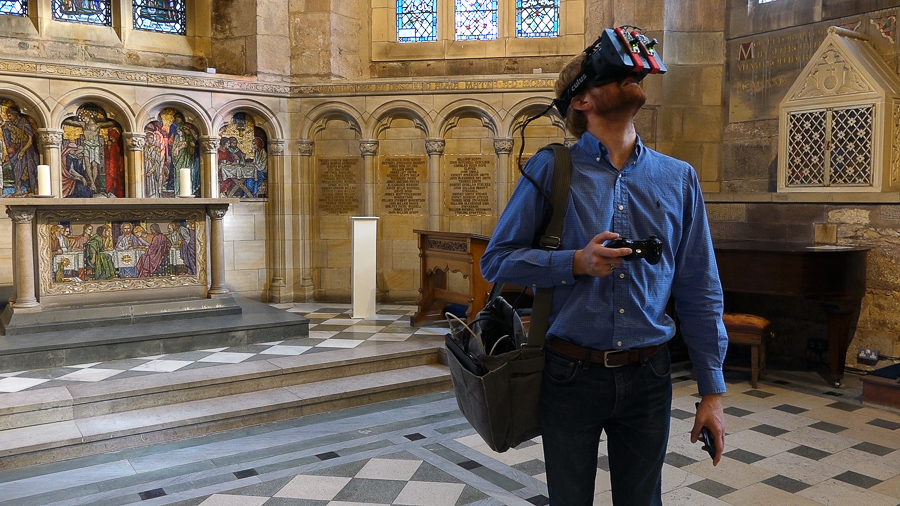
\includegraphics[width=\linewidth]{participant-m.png}
		\caption{participant-m.png}
		\label{participant-m.png}
	\end{center}
\end{figure}

Studies are split into three parts; Phase 1, Phase 2.1 \& Phase 2.2.

\section{The Case for Mobile XR}
This investigation compares two scenarios for interaction with a real location \& a corresponding virtual location.

\begin{enumerate}
	\item \textbf{Stationary scenario} - interacting with the virtual location from a fixed real location, then subsequently interacting with the real location.
	\item \textbf{Mobile scenario} - using the Mirrorshades platform to interact with both the real location \& the corresponding virtual location in tandem, whilst moving around both environments.
\end{enumerate}

The locations in question are St Salvator's chapel \& a virtual reconstruction of the chapel as it stood in 1450-1460. The stationary scenario is representative of how virtual reality technologies, including both CAVEs \& HMDs, have previously been used for dissemination of virtual reality content in cultural heritage contexts~\cite{Roussou2002} \& thus this investigation serves to compare Mirrorshades with previous applications virtual reality content to these contexts.

\section{Process}
\begin{itemize}
	\item Participants complete a pre-task questionnaire, which provides calibration for their subsequent responses by enquiring about age, gender identity, previous experience with VR hardware \& previous interactions with either the real or virtual chapel. This questionnaire is included as Appendix \ref{pre_task_questionnaire}.
	
	\item Participants familiarise themselves with the experience of using the Oculus Rift DK1 HMD \& the Xbox 360 controller by interacting with the `Tuscany demo' prepared \& maintained by the Oculus VR team. This is performed from a seated position.
	
	\item Participants complete the stationary scenario.
	
	\item After completing the stationary scenario, participants complete the System Usability Scale (SUS)~\cite{Brooke1996} questionnaire, included as Appendix \ref{sus} \& a 12-item questionnaire, included as Appendix \ref{12_questions}.
	
	\item Participants complete the mobile scenario.
	
	\item After completing the mobile scenario, participants complete the SUS questionnaire \& the 12-item questionnaire again.
	
	\item Finally, the participant is engaged in a short structured interview. Interview prompts are included as Appendix \ref{interview_questions}.
\end{itemize}

In addition to SUS, the 12-item questionnaire \& the structured interview, quantitative data is logged by the Mirrorshades platform when a participant is interacting with virtual content in the first scenario \& at all times during the second scenario.

\section{The Scenarios}
Both scenarios that participants complete for this investigation are designed to mimic the style of exploration \& interaction that visitors to the chapel display, which was observed over several occasions. Visitors enter the chapel from the North/West corner then proceed to walk Eastwards along the nave, pausing to look around after passing through the rood screen, before continuing along the nave toward the altar. Visitors pause in front of the alter upon reaching the end of the pews \& then walk North toward the tomb where they pause again to inspect it. Participants are instructed to imagine that they are performing a similar visit to the chapel \& to follow a similar path, pausing after the rood screen, at the end of the pews \& in front of the tomb. Participants are shown the map included as figure \ref{chapel_path} to explain the scenario better.

In the stationary scenario, participants interact with the virtual chapel using the Rift \& Xbox controller, whilst in a sitting position. After completing the path, they remove the headset \& then walk the same path in the real chapel. This scenario alludes to how virtual reality technologies have previously been applied to cultural heritage situations, allowing visitors to experience a virtual reality reconstruction or reimagination of the real environment from a fixed position \& with their view of the real environment wholly occluded by their view of the virtual environment.

In the mobile scenario, participants wear the HMD, hold the Xbox controller in their right hand \& the smartphone in their left, with the laptop \& battery pack in a satchel worn over the right shoulder. They then walk the same path, but this time with the ability to transition at any time between viewing the real environment \& the virtual environment from the same vantage point.

In this first investigation phase, only one transition is available to participants. Preliminary experiments involving the researchers' colleagues that allowed hard transitions, linear interpolated transitions \& analogue selectable opacity, indicated that the linear interpolated transition was preferred to either the hard transition or the analogue selectable opacity \& thus this is the transition available to participants in this first phase investigation.

\begin{figure}[h]
	\begin{center}
		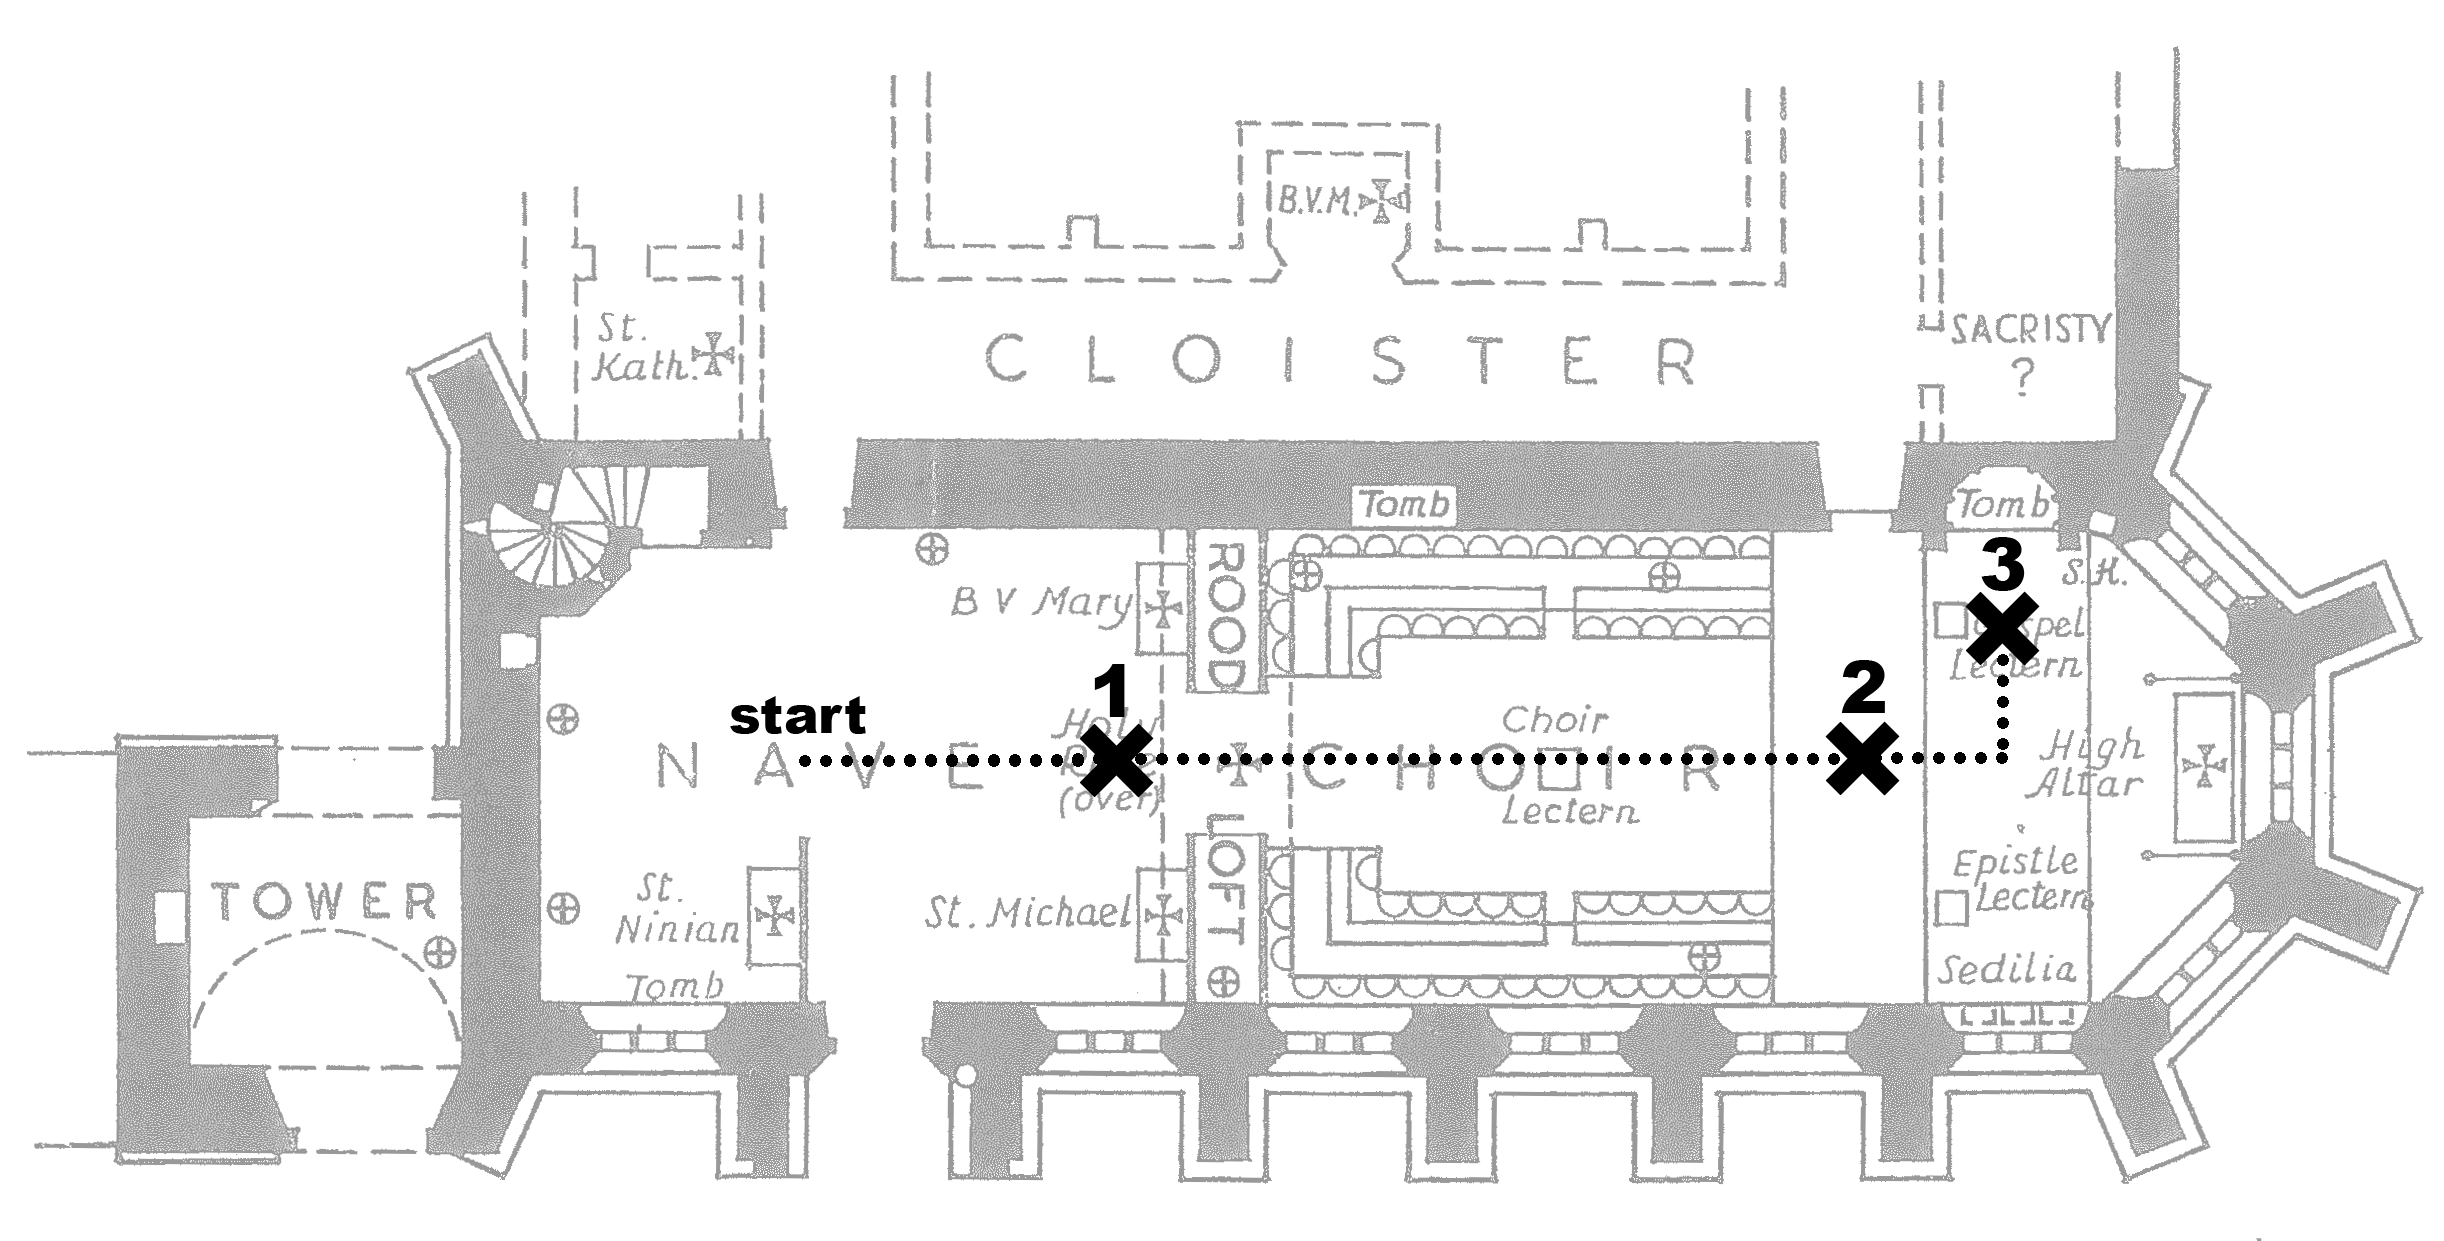
\includegraphics[width=\linewidth]{chapel-path.png}
		\caption{The path \& positions within the chapel that participants are instructed to attend to.}
		\label{chapel-path}
	\end{center}
\end{figure}

\section{Hypotheses}
The aim of the mobile scenario is to improve participant engagement with \& understanding of the relationships between the real \& virtual environments, by addressing the problems of spatial \& temporal separation inherent with the `traditional' stationary scenario, by imparting upon the participant the ability to transition between equivalent vantage points within the real \& virtual environments at will.

While we expect participants to report that the mobile scenario does indeed allow them to better compare \& contrast the real \& virtual environments, identify differences between the real \& virtual environments \& gain a better understanding of how the real \& virtual environments relate to each other, we expect some participants to report that having to `split' their attention between the two environments in the mobile scenario leads to lessened engagement \& understanding \& that the visual quality of the real view through the headset/cameras leads to some participants preferring to interact with the real environment without the headset.

We expect the cumbersome nature of the mobile scenario \& the reduced quality of viewing the real environment via the headset/cameras to have a noticeable effect upon participants movement (both position \& head orientation) in the mobile scenario.

Addressing these issues, such that participants don't find viewing the real through the headset to be such a reduction in quality compared to just seeing real, such that participants feel as though they can move \& look around themselves as much in the mobile scenario as in the stationary scenario \& such that participants transition between real \& virtual at any time instead of avoiding transitions in situations in which they think that they will be unpleasant/jarring, is key \& what the next stage will focus on.

%Engagement with individual environments will be lessened
%Engagement with both environments will be increased
%So for tasks where real time comparison \& contrast is required, this is good

\section{SUS}
SUS scores for the mobile scenario are expected to average lower than those for the stationary scenario, due to the cumbersome nature of the platform when performing the mobile scenario; during the stationary scenario, participants are seated, whilst during the mobile scenario they are required to carry a satchel over one shoulder \& hold a smartphone in their left hand. Participants who are able to overcome this cumbersomeness are expected to respond more favourably to the mobile scenario than those who cannot overcome it.

\section{12-item Questionnaire}
\begin{itemize}
	\item Participants will find it easier to compare \& contrast real \& virtual environments in the mobile scenario than in the stationary scenario (q2)
	\item Participants will experience a greater  sense of `being in' the virtual environment in the mobile scenario than in the stationary scenario (q4, due to physical movement/embodiment)
	\item Participants will have a greater sense of `being in the past' in the mobile scenario than in the stationary scenario (q7)
	\item Participants will maintain greater awareness of both real \& virtual environments in the mobile scenario than in the stationary scenario (q5)
%	\item Participants will notice more differences between real \& virtual environments in the mobile scenario than in the stationary scenario (q10)
	\item Participants will gain a better understanding of what the chapel was like in the past in the mobile scenario than in the stationary scenario (q12)
\end{itemize}

\section{Log data}
\begin{itemize}
	\item Head movement (pitch \& yaw) will be more restricted in the mobile scenario compared to the stationary scenario
	\item Aversion to looking around (even at real) when moving in the mobile scenario
	\item Head movements will be larger discrete changes in the stationary scenario compared to the mobile scenario
	\item Tendency to only look at virtual when looking around
\end{itemize}

\section{Interviews}
\begin{itemize}
	\item mobile scenario makes it easier to spot differences
	\item mobile scenario reveals differences that stationary didn't
	\item stationary does not reveal differences that mobile doesn't
	\item mobile scenario is preferred \& is user-reported as 'more engaging'
\end{itemize}

%=========================================================================================================

\section{Phase 1 Results}

\subsection{Pre-task Questionnaire}

For n=5 ages ranged from 21-26, 3x female \& 2x male, all reported previous experience using a games console controller, 1x reported previous use of a HMD, 2x reported having previously visited the chapel, none had previously interacted with the virtual chapel model.

%0 = false
%1 = true

%+------+------+------+------+------+------+------+
%| id   | q1   | q2   | q3   | q4   | q5   | q6   |
%+------+------+------+------+------+------+------+
%|    1 |   25 | f    |    1 |    1 |    1 |    0 |
%|    2 |   21 | m    |    1 |    0 |    0 |    0 |
%|    3 |   26 | m    |    1 |    0 |    0 |    0 |
%|    4 |   22 | f    |    1 |    0 |    1 |    0 |
%|    5 |   23 | f    |    1 |    0 |    1 |    0 |
%+------+------+------+------+------+------+------+

\pagebreak

\subsection{SUS}

\begin{figure}[h]
	\begin{center}
		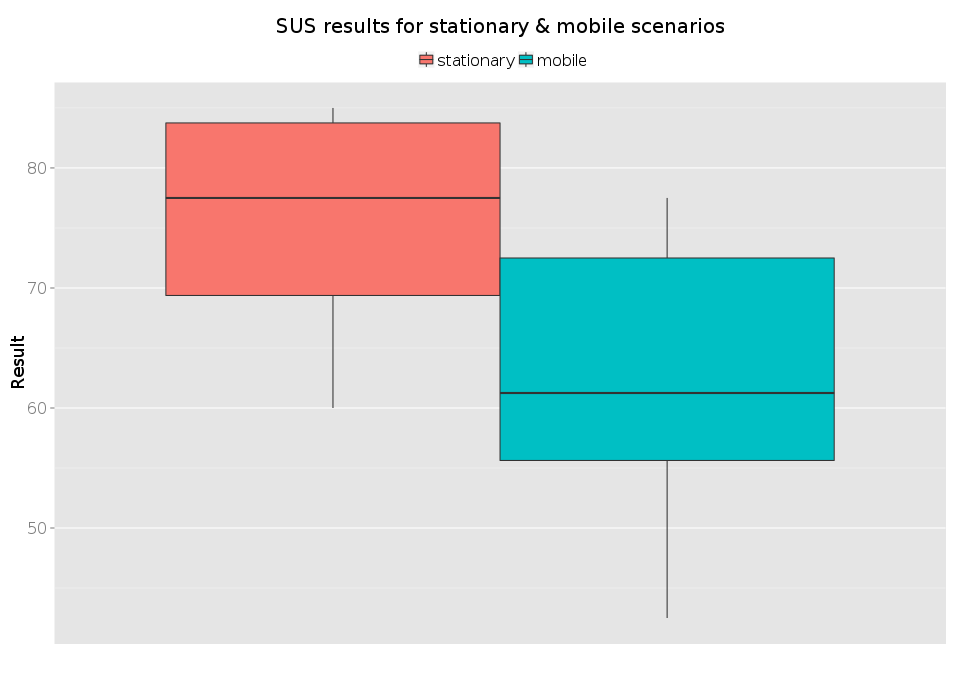
\includegraphics[width=0.7\linewidth]{1/sus.png}
		\caption{SUS results.}
		\label{sus}
	\end{center}
\end{figure}

As expected, the SUS scores for the mobile scenario are lower than those of the stationary scenario, although not drastically so. Furthermore, although scoring lower on SUS, the mobile scenario came out above the stationary scenario when looking at the results of q8 in the 12-item questionnaire which asked participants if they thought they would have preferred a conventional computer monitor.

\pagebreak

\subsection{12-item Questionnaire}

\begin{figure}[h]
	\begin{center}
		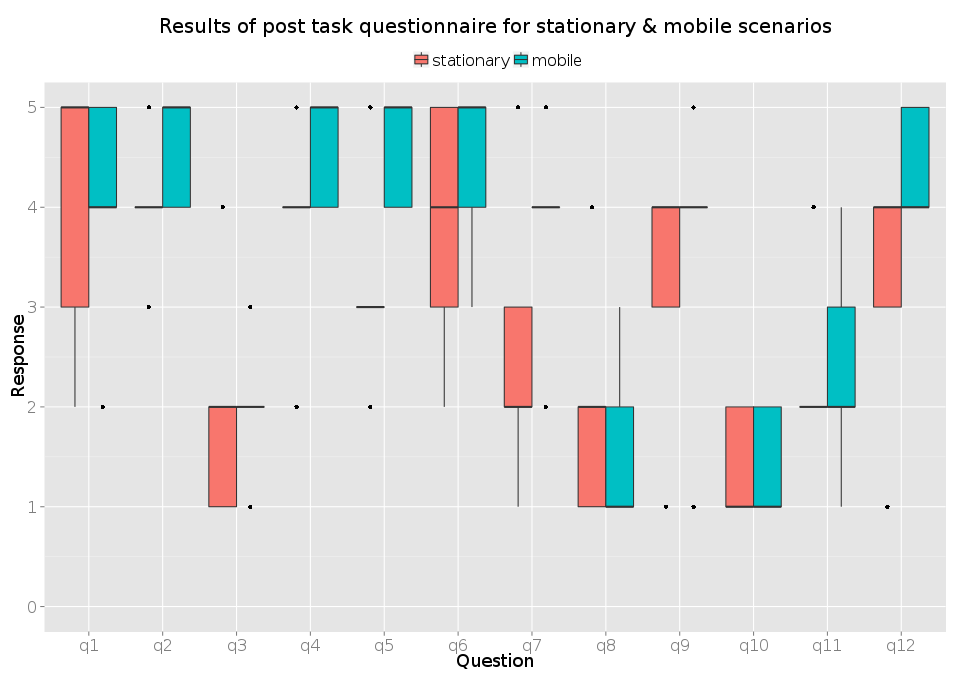
\includegraphics[width=0.9\linewidth]{1/post_task_questionnaire_boxplot.png}
		\caption{12-item questionnaire results.}
		\label{12-item_boxplot}
	\end{center}
\end{figure}

The hypotheses seem to hold, in particular;

\begin{itemize}
	\item \textit{Participants will maintain greater awareness of both real \& virtual environments in the mobile scenario than in the stationary scenario} is supported by the responses to q5
	\item \textit{Participants will have a greater sense of `being in the past' in the mobile scenario than in the stationary scenario} is supported by q7 (thanks to embodiment?)
	\item \textit{Participants will gain a better understanding of what the chapel was like in the past in the mobile scenario than in the stationary scenario} is supported by q12
\end{itemize}

It is worth highlighting the responses to q10 in relation to those to q2. Participants reported finding it easier to compare features from the past \& present (q2) during the mobile scenario, however did not report a difference between not noticing differences between the real \& virtual environments (q10).

%=========================================================================================================

\clearpage

\subsection{Participant 1}

\begin{figure}[h]
	\makebox[\textwidth][c]{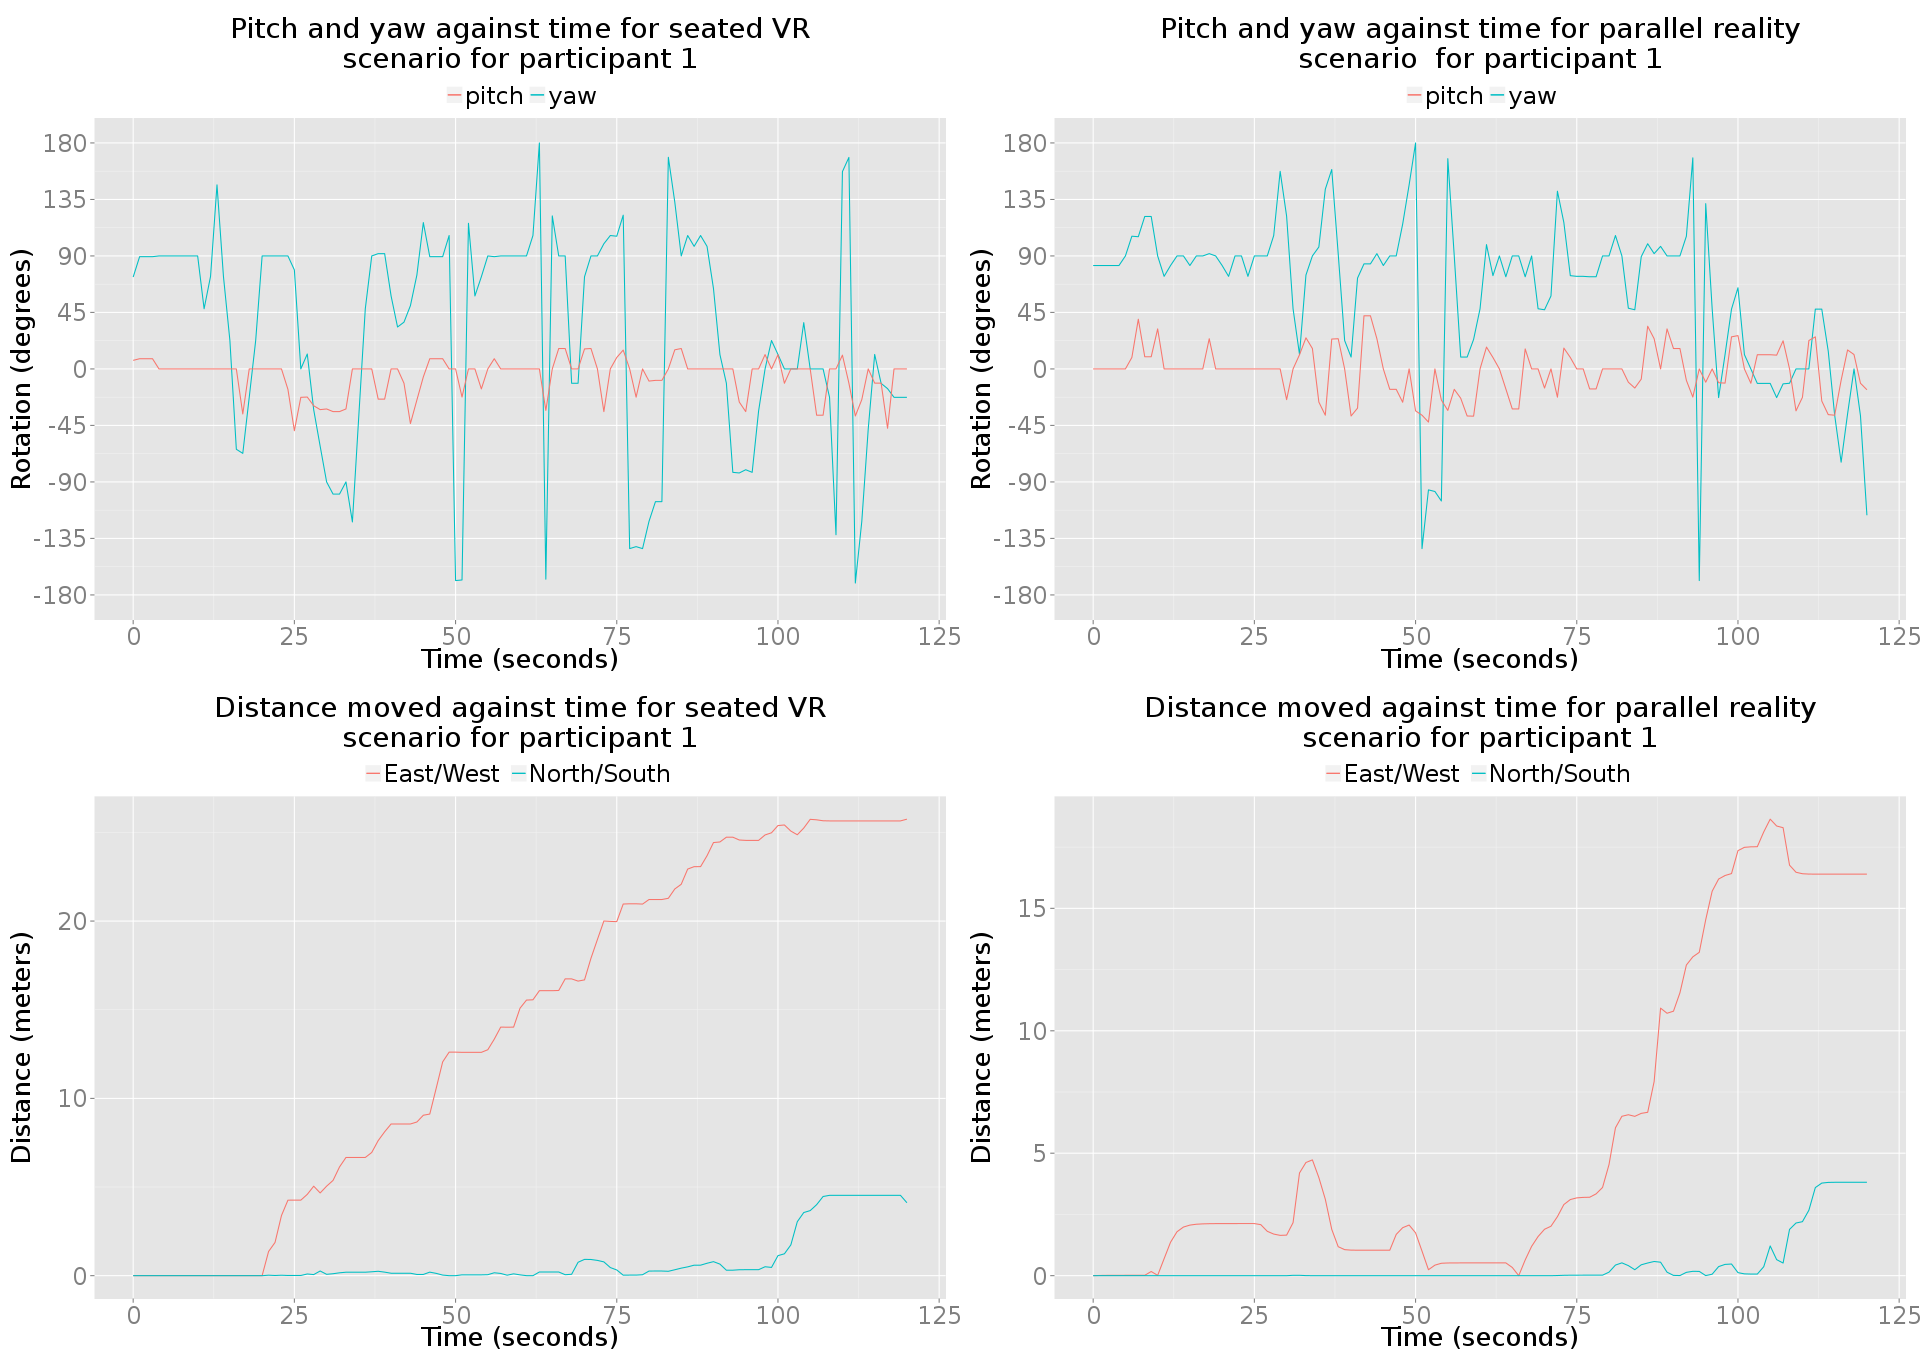
\includegraphics[width=1.2\textwidth]{1/1_4up.png}}
	\caption{Some images, yah.}
\end{figure}

\clearpage

\begin{figure}[h]
	\makebox[\textwidth][c]{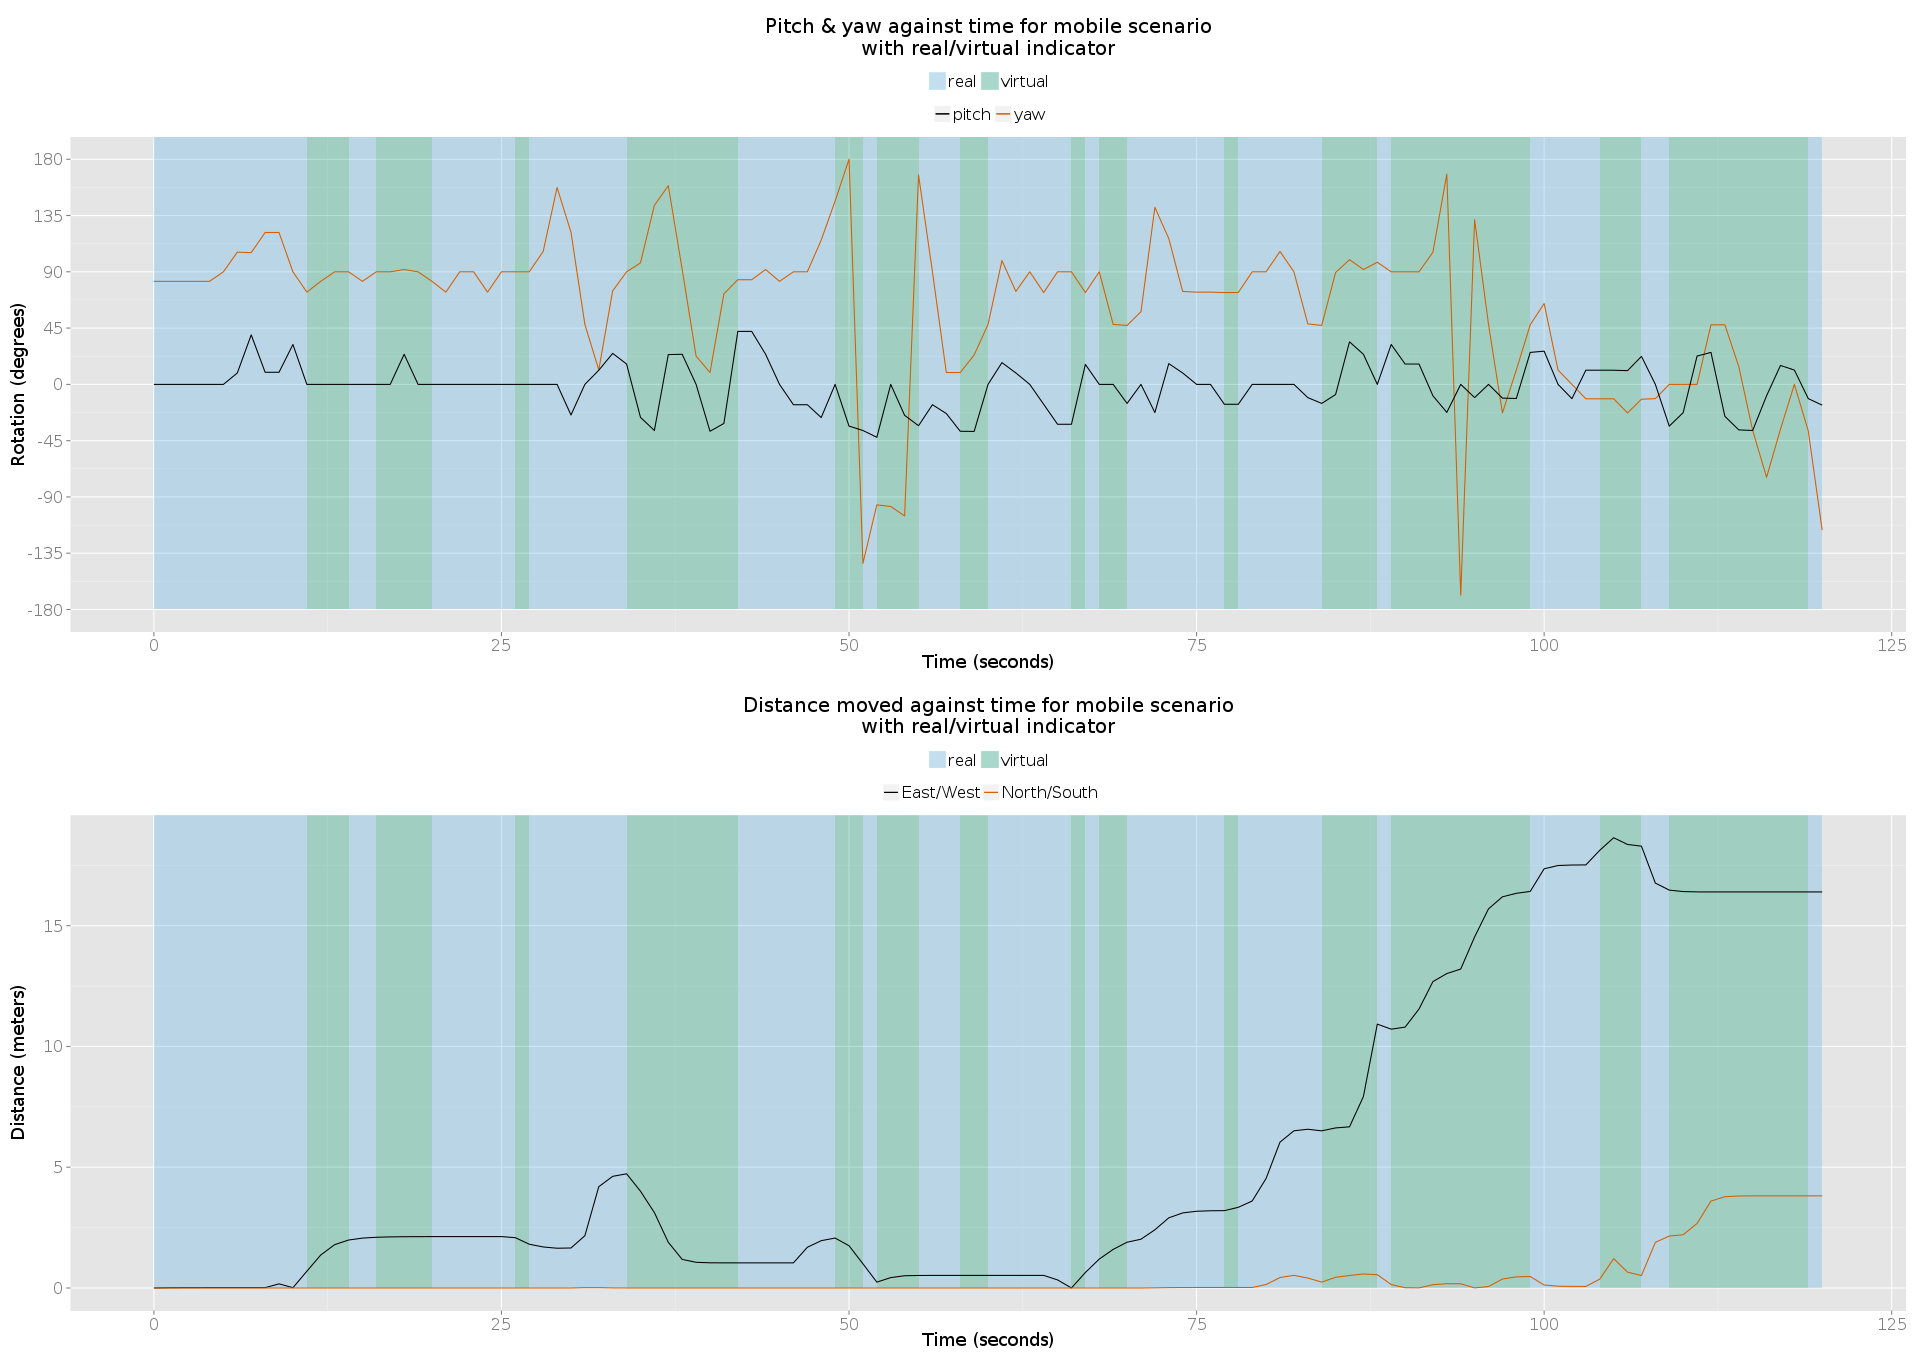
\includegraphics[width=1.2\textwidth]{1/1_2up.png}}
	\caption{Some images, yah.}
\end{figure}

%=========================================================================================================

\clearpage

\subsection{Participant 3}

\begin{figure}[h]
	\makebox[\textwidth][c]{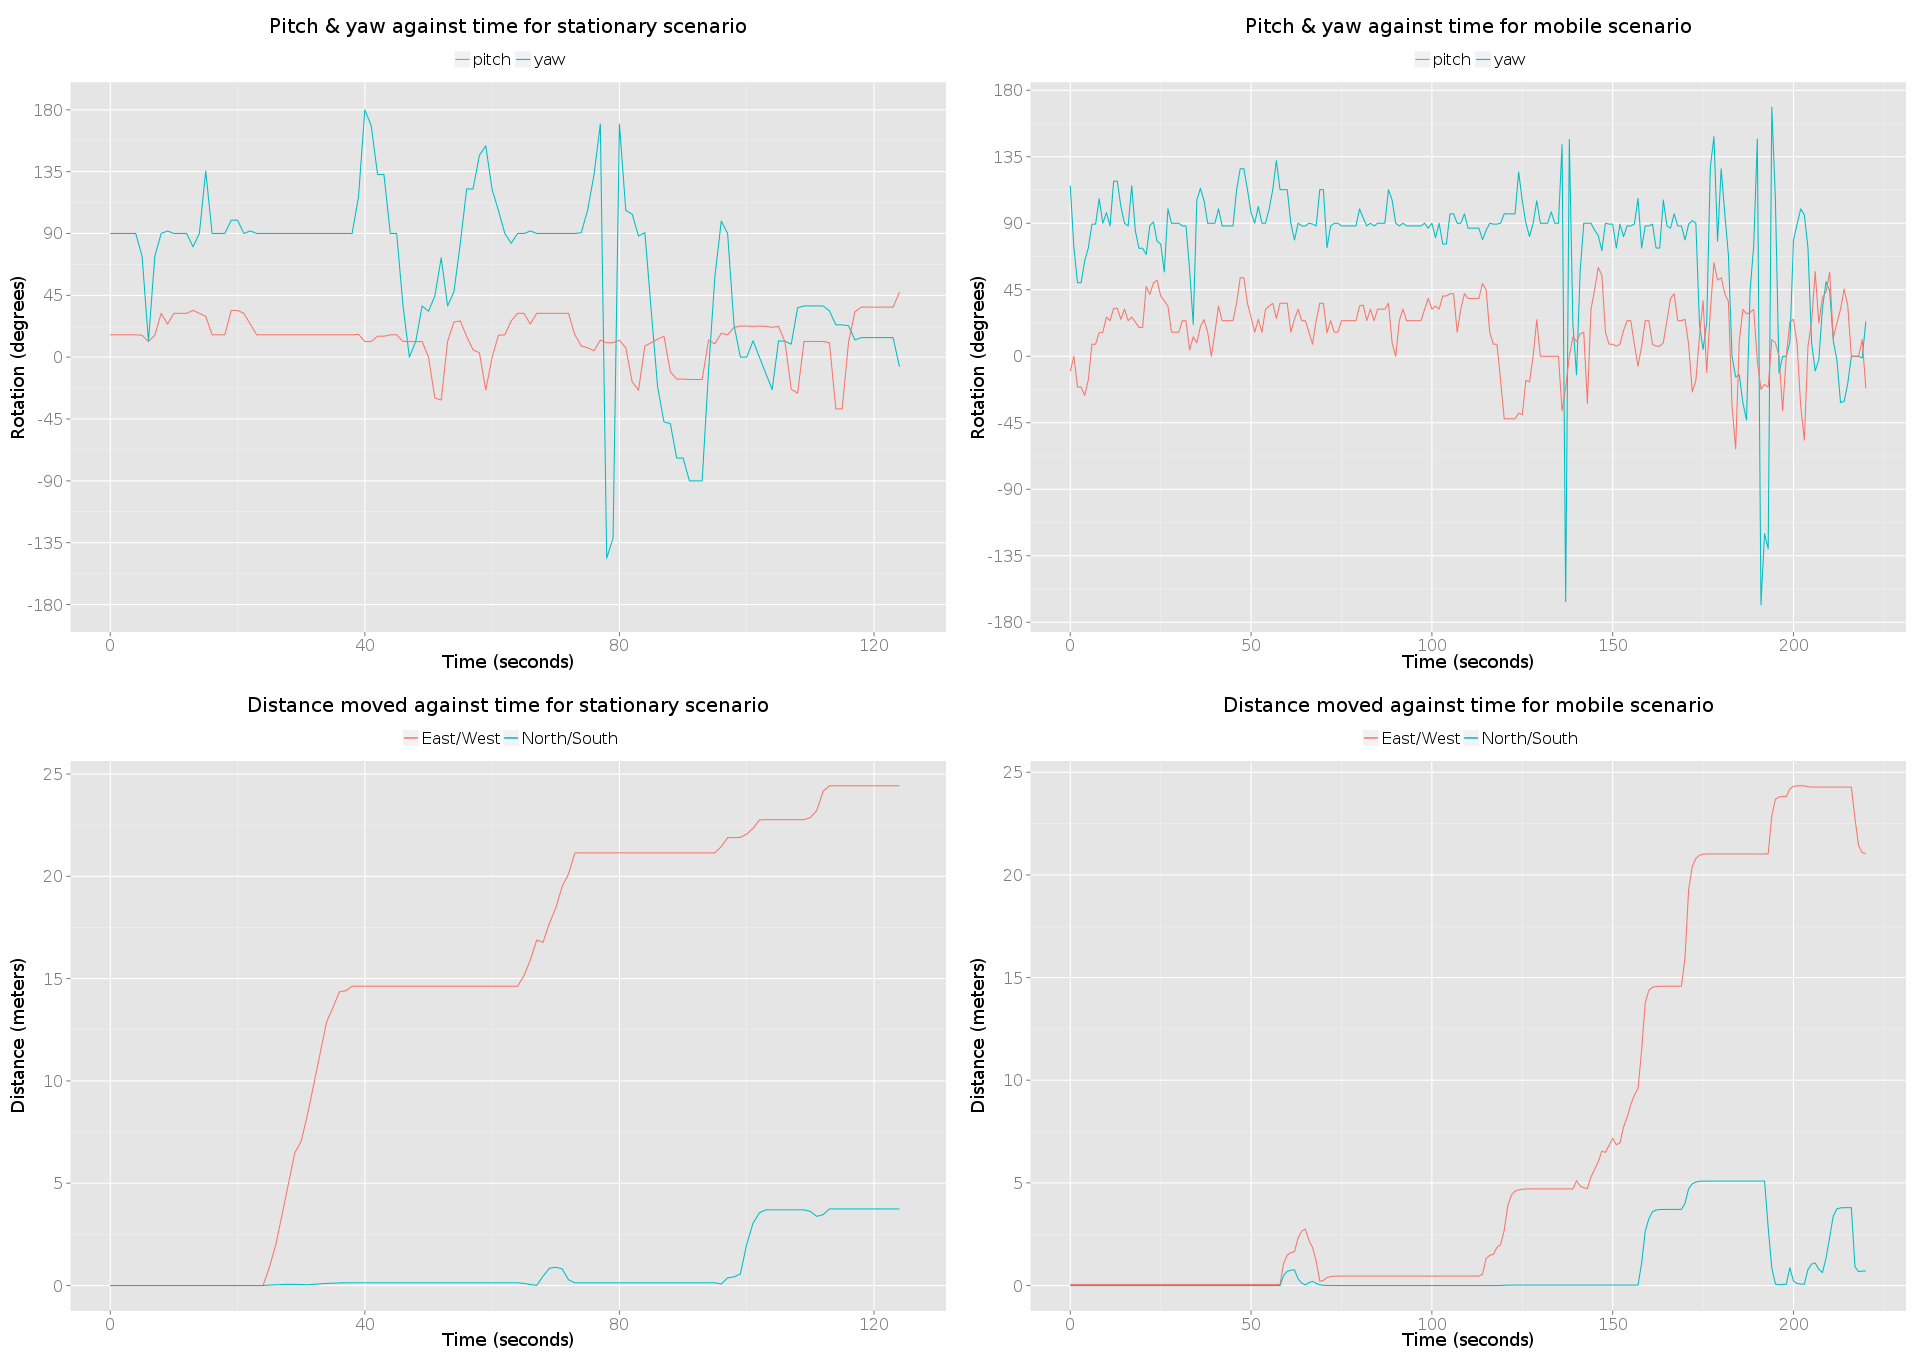
\includegraphics[width=1.2\textwidth]{1/3_4up.png}}
	\caption{Some images, yah.}
\end{figure}

\clearpage

\begin{figure}[h]
	\makebox[\textwidth][c]{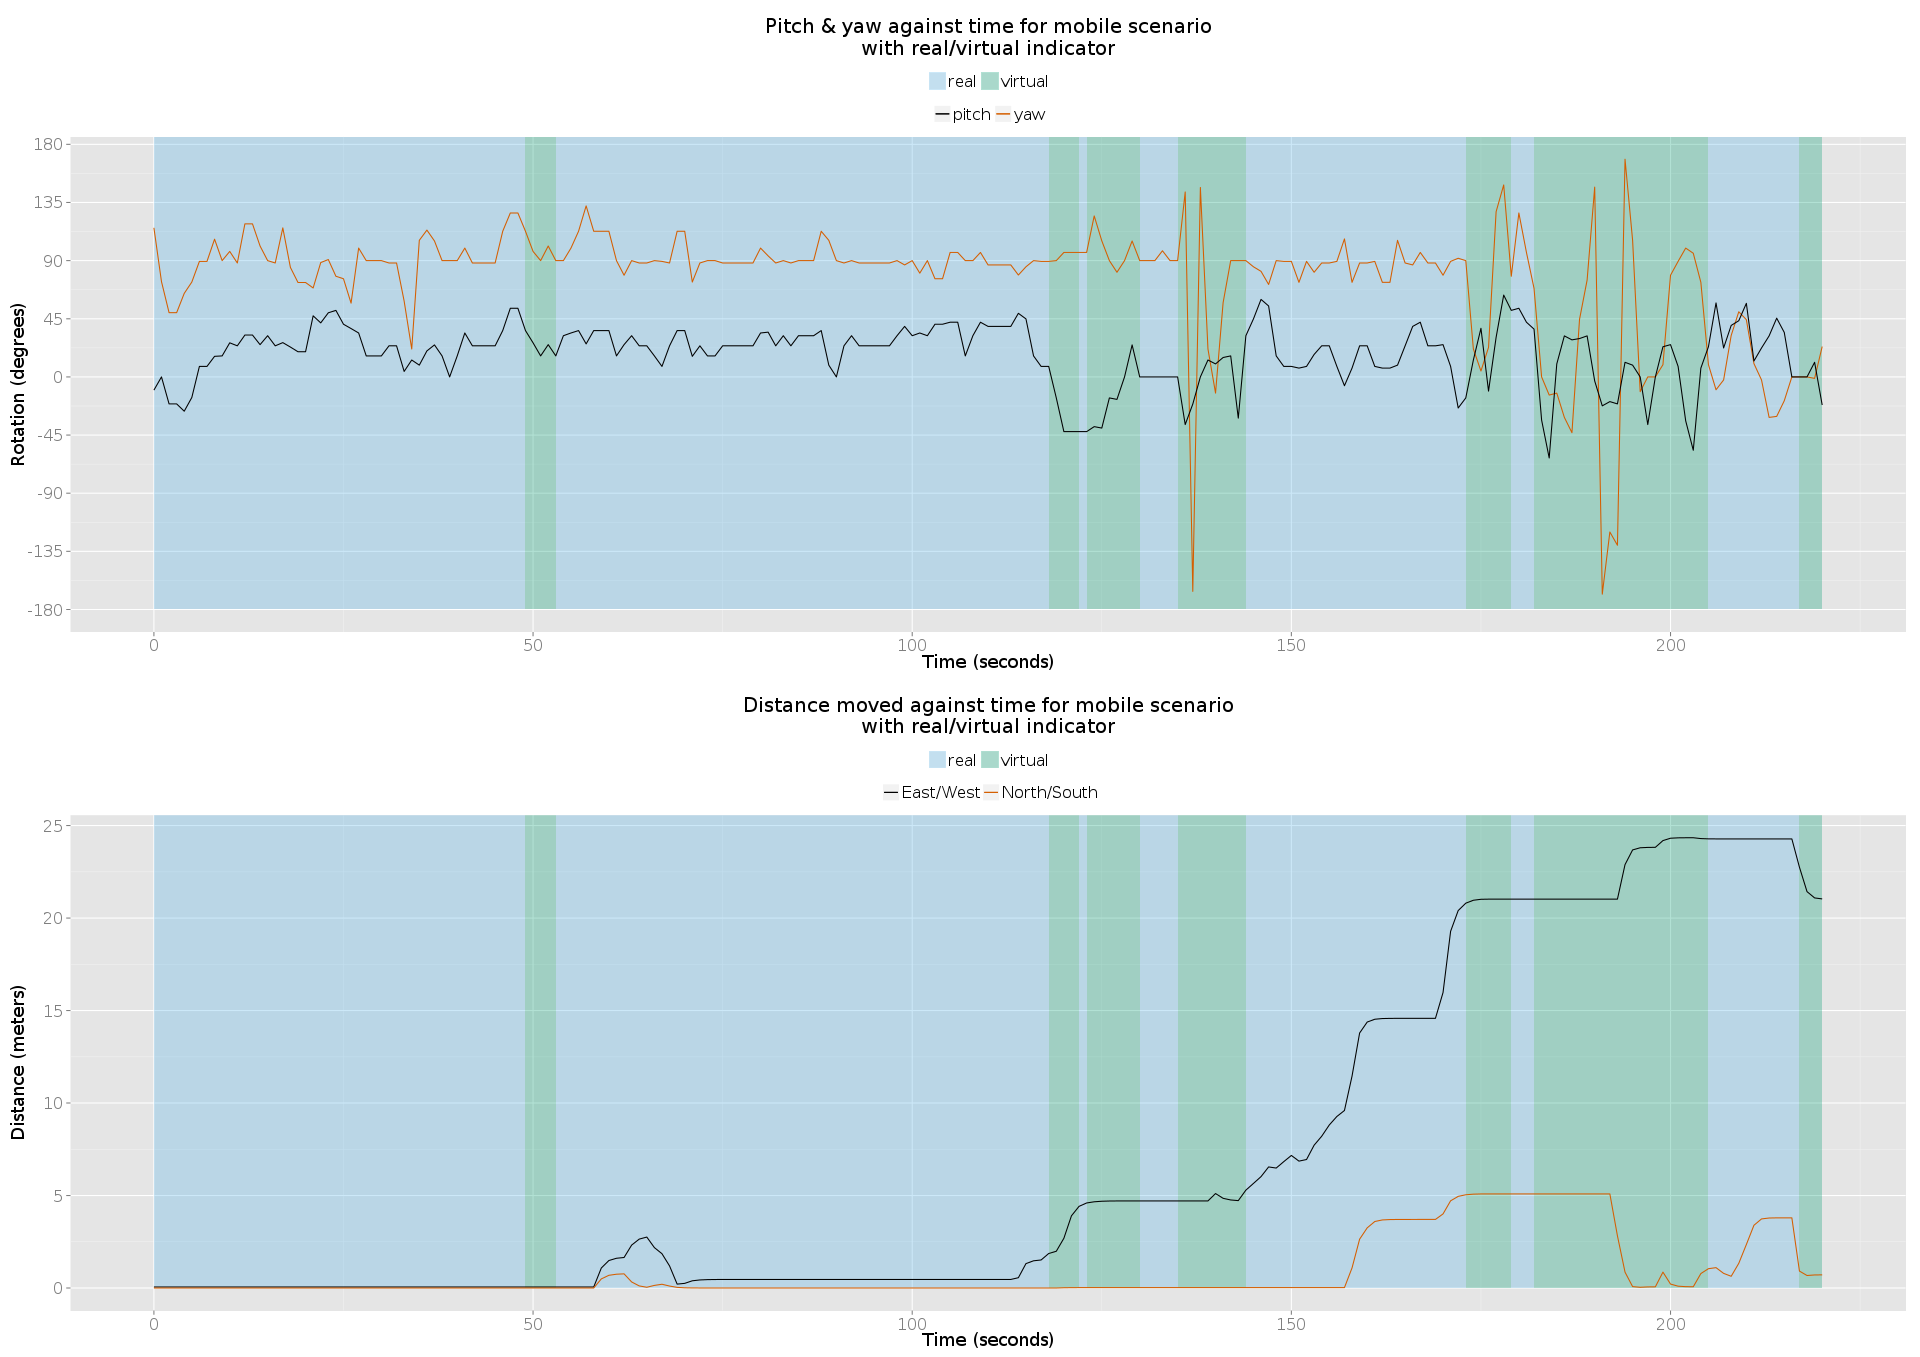
\includegraphics[width=1.2\textwidth]{1/3_2up.png}}
	\caption{Some images, yah.}
\end{figure}

%=========================================================================================================

\clearpage

\subsection{Participant 4}

\begin{figure}[h]
	\makebox[\textwidth][c]{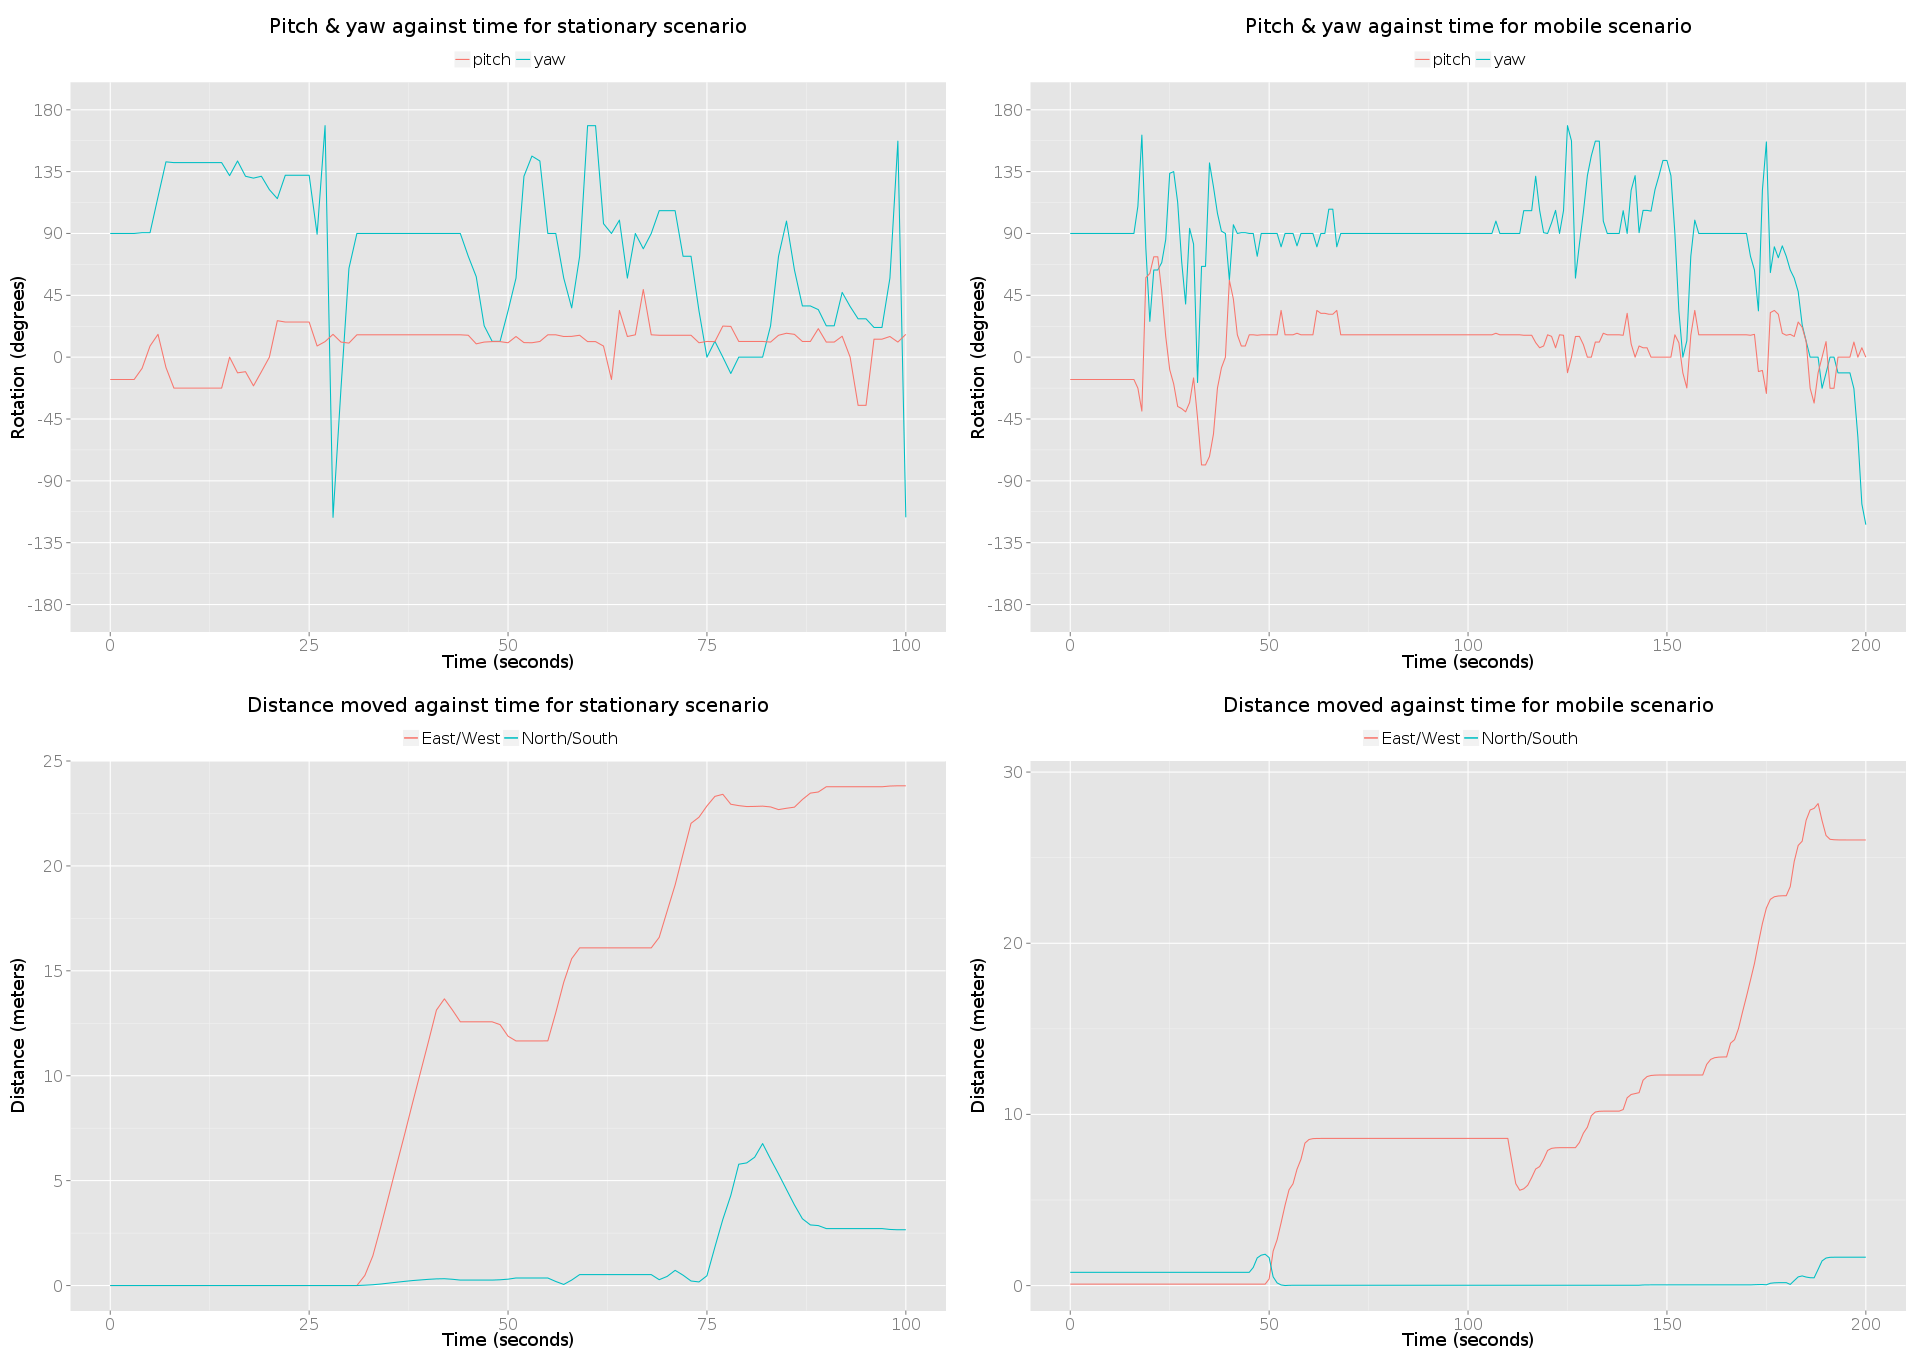
\includegraphics[width=1.2\textwidth]{1/4_4up.png}}
	\caption{Some images, yah.}
\end{figure}

\clearpage

\begin{figure}[h]
	\makebox[\textwidth][c]{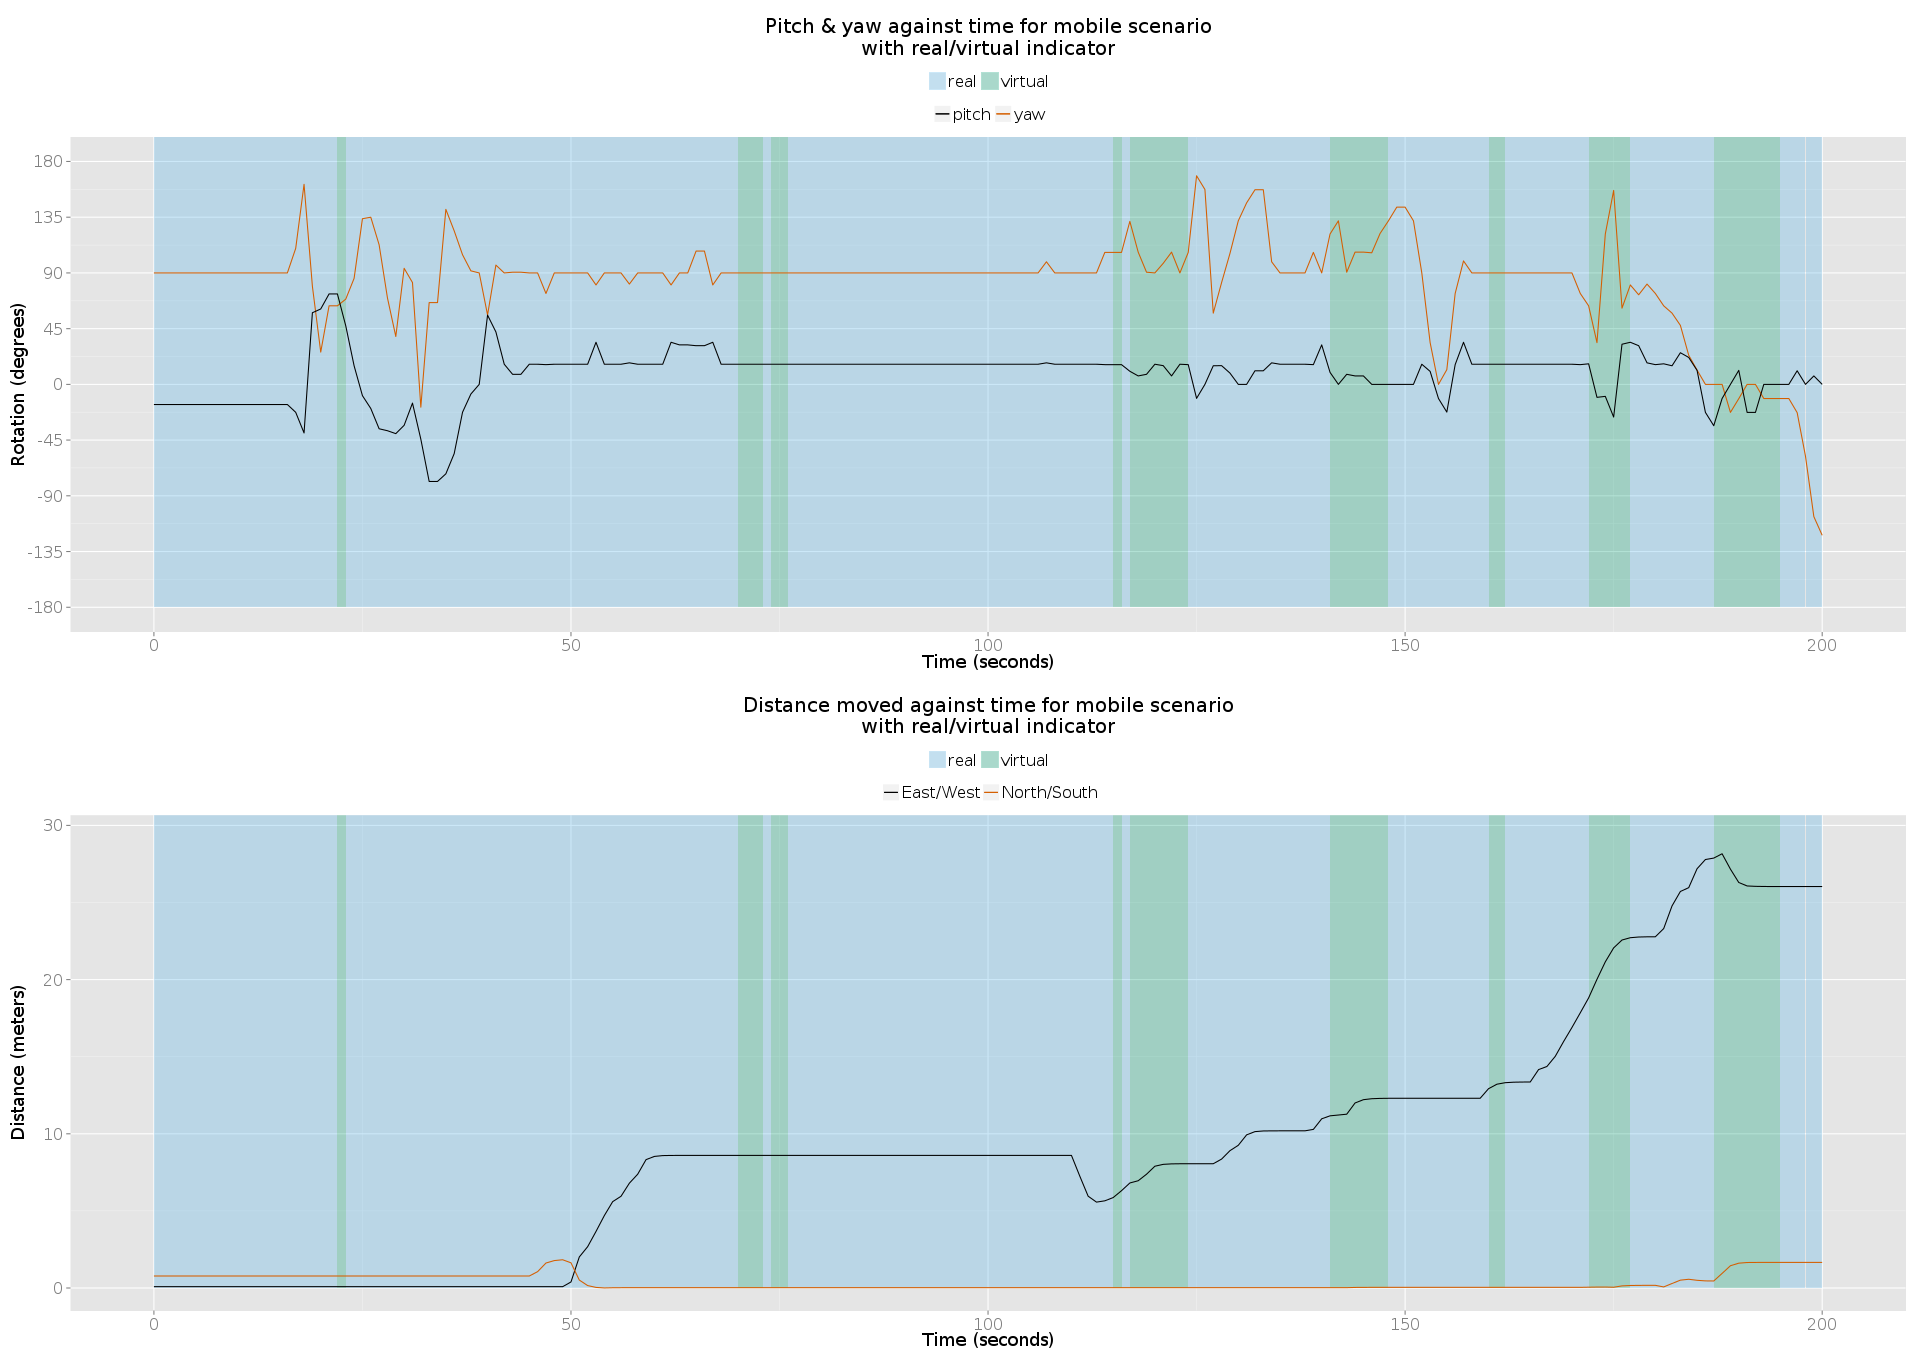
\includegraphics[width=1.2\textwidth]{1/4_2up.png}}
	\caption{Some images, yah.}
\end{figure}

%=========================================================================================================

\subsection{Participant 5}

\clearpage

\begin{figure}[h]
	\makebox[\textwidth][c]{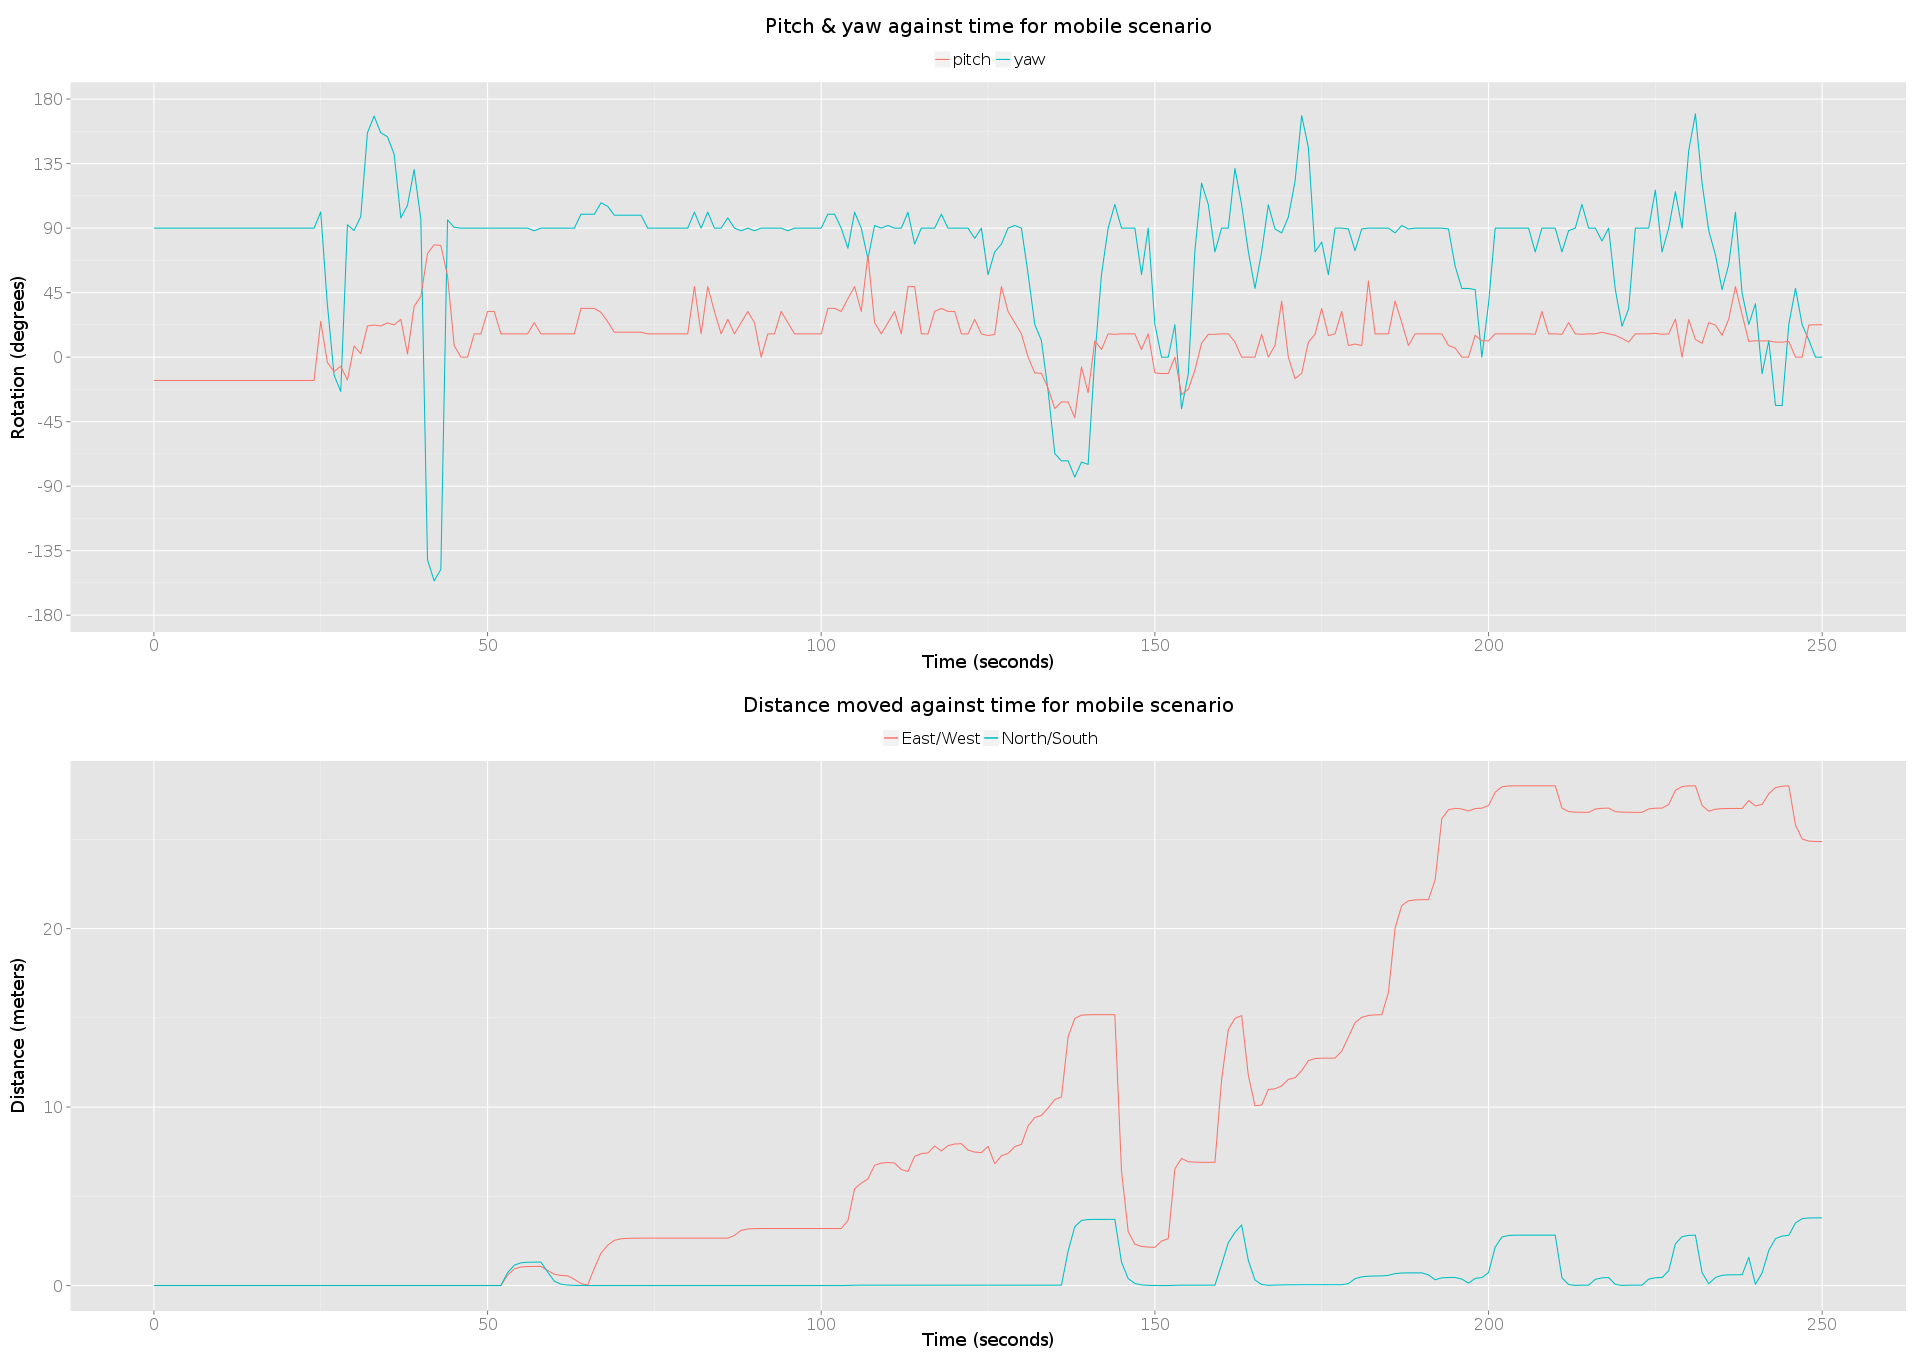
\includegraphics[width=1.2\textwidth]{1/5_4up.png}}
	\caption{Some images, yah.}
\end{figure}

\clearpage

\begin{figure}[h]
	\makebox[\textwidth][c]{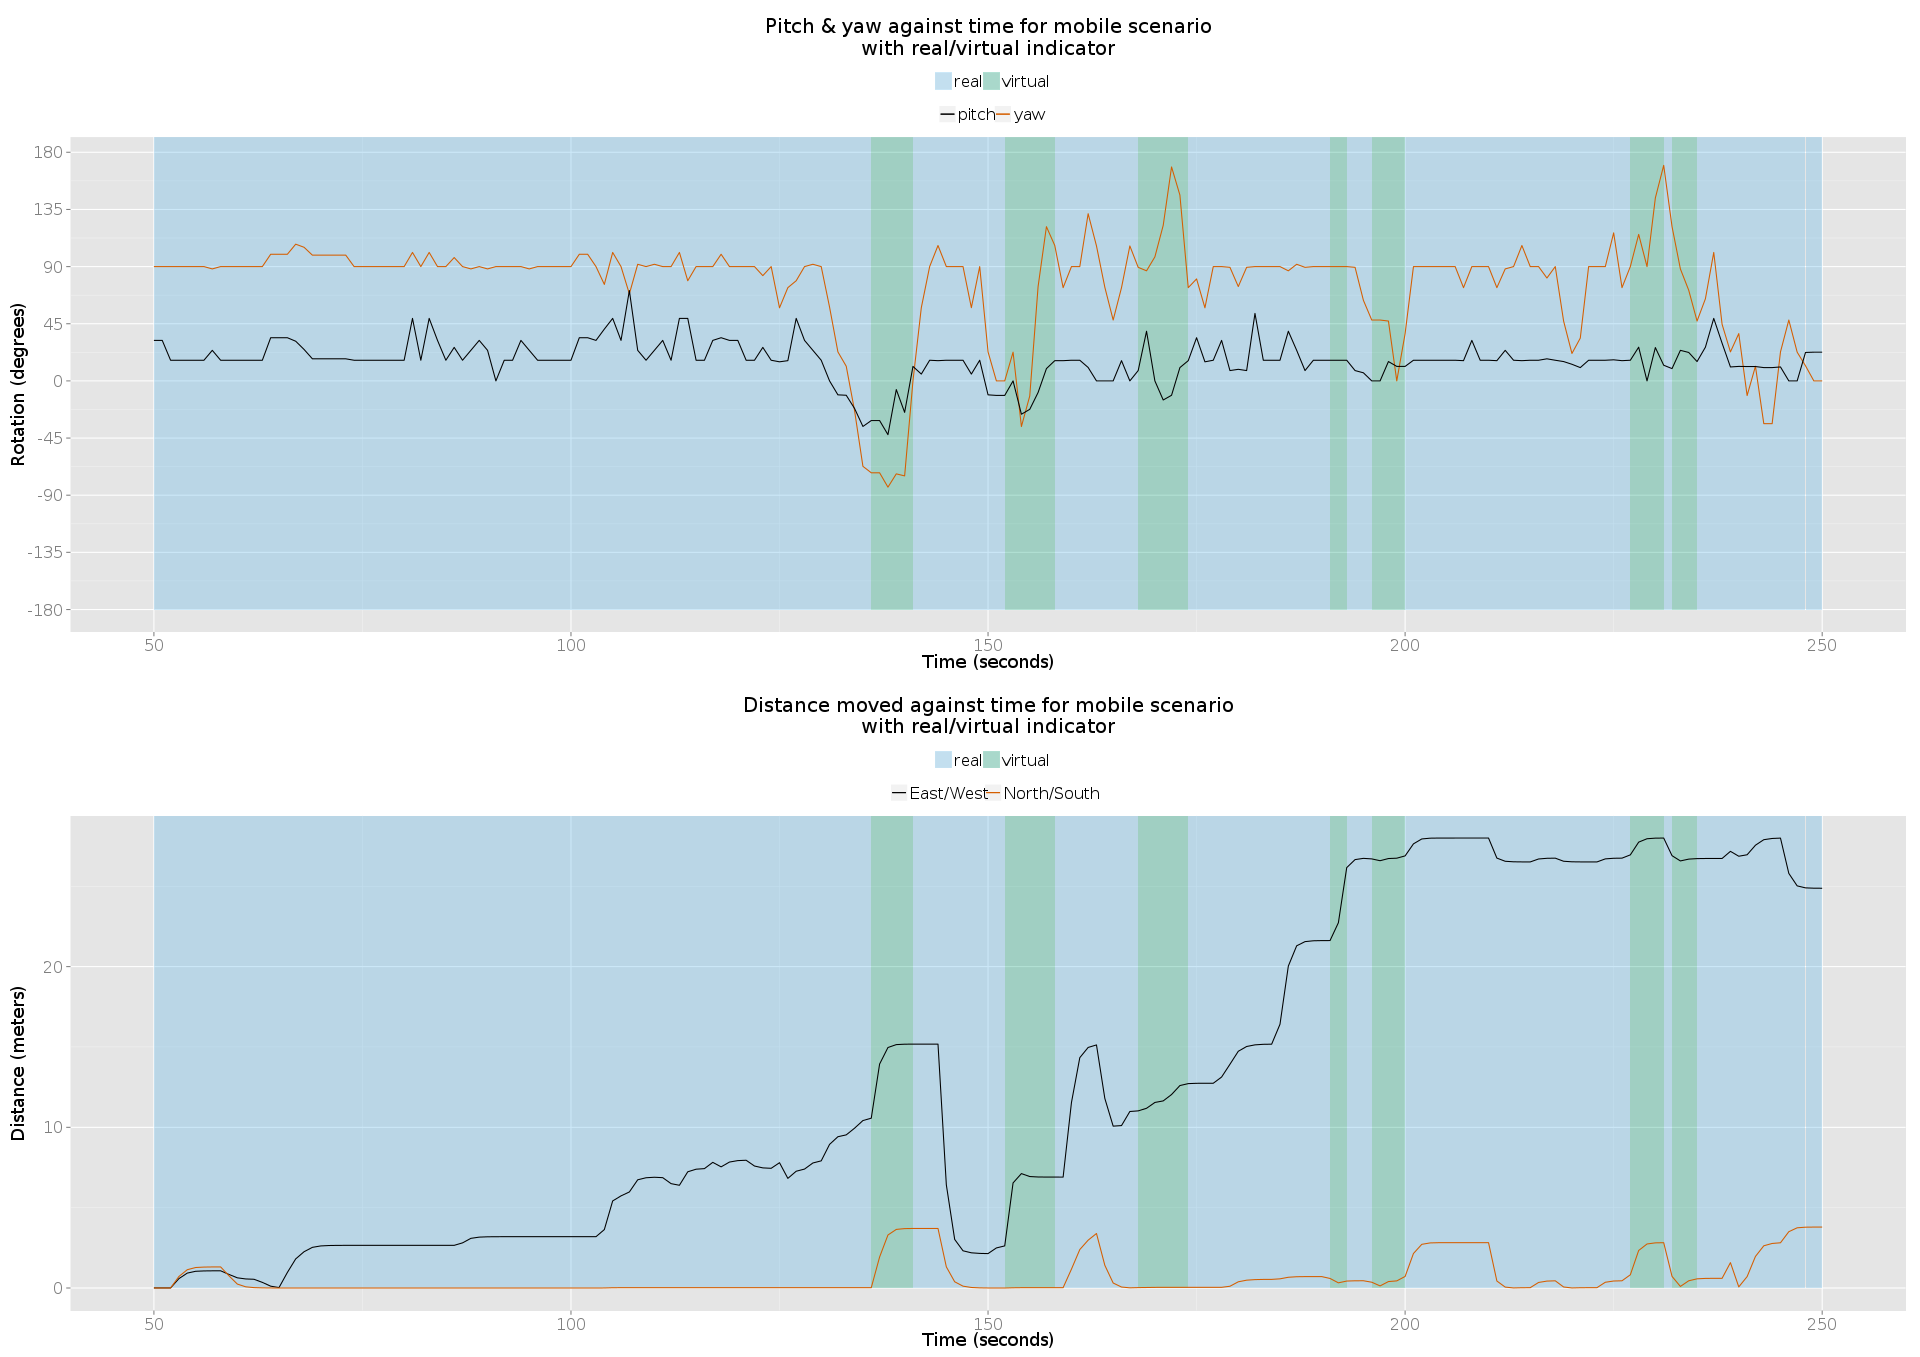
\includegraphics[width=1.2\textwidth]{1/5_2up.png}}
	\caption{Some images, yah.}
\end{figure}

%=========================================================================================================

\subsection{Participant 6}

\clearpage

\begin{figure}[h]
	\makebox[\textwidth][c]{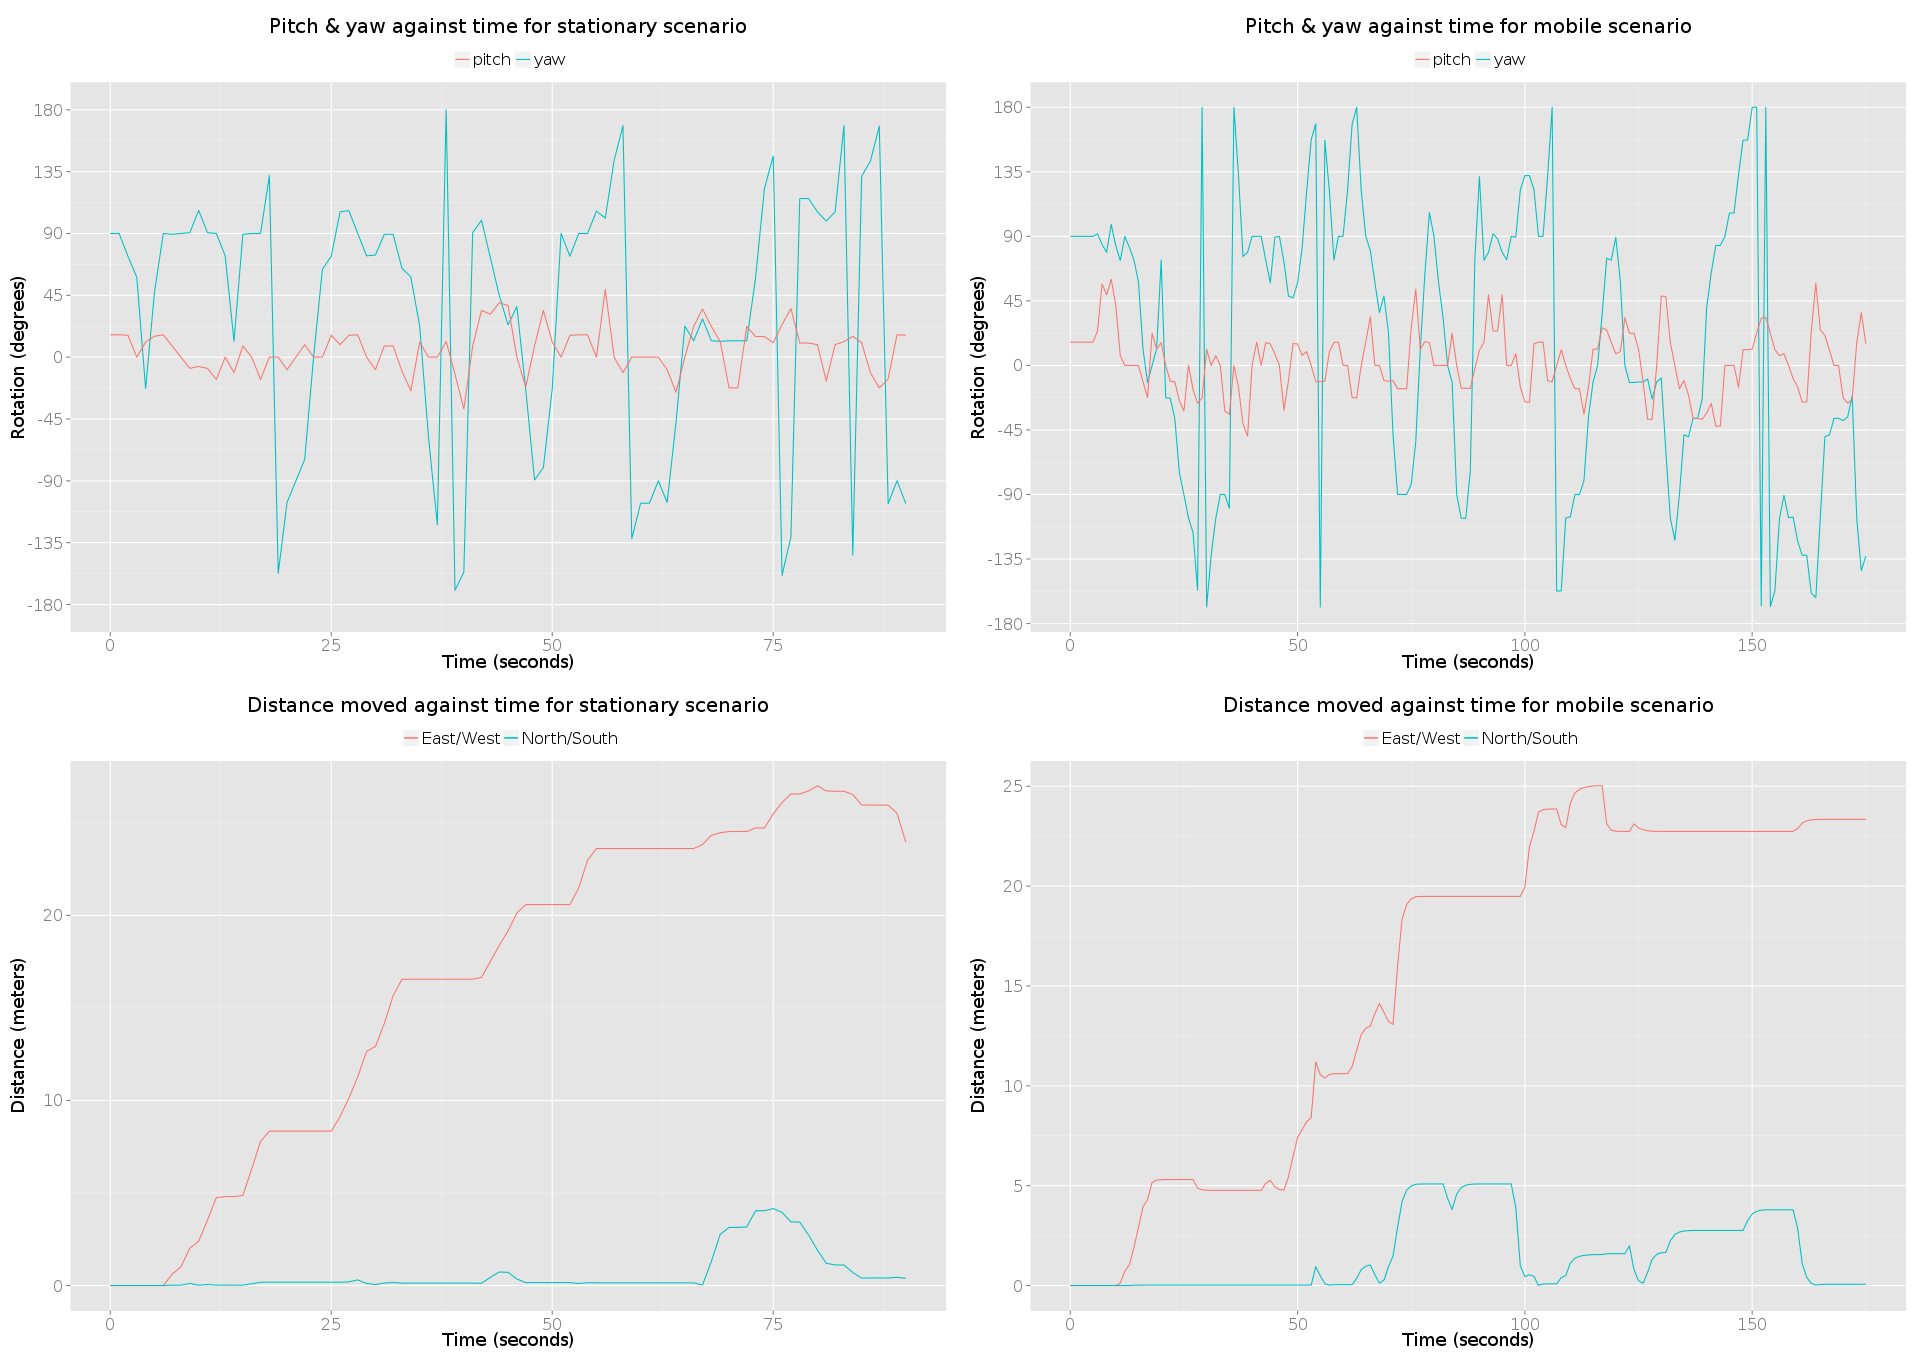
\includegraphics[width=1.2\textwidth]{1/6_4up.png}}
	\caption{Some images, yah.}
\end{figure}

\clearpage

\begin{figure}[h]
	\makebox[\textwidth][c]{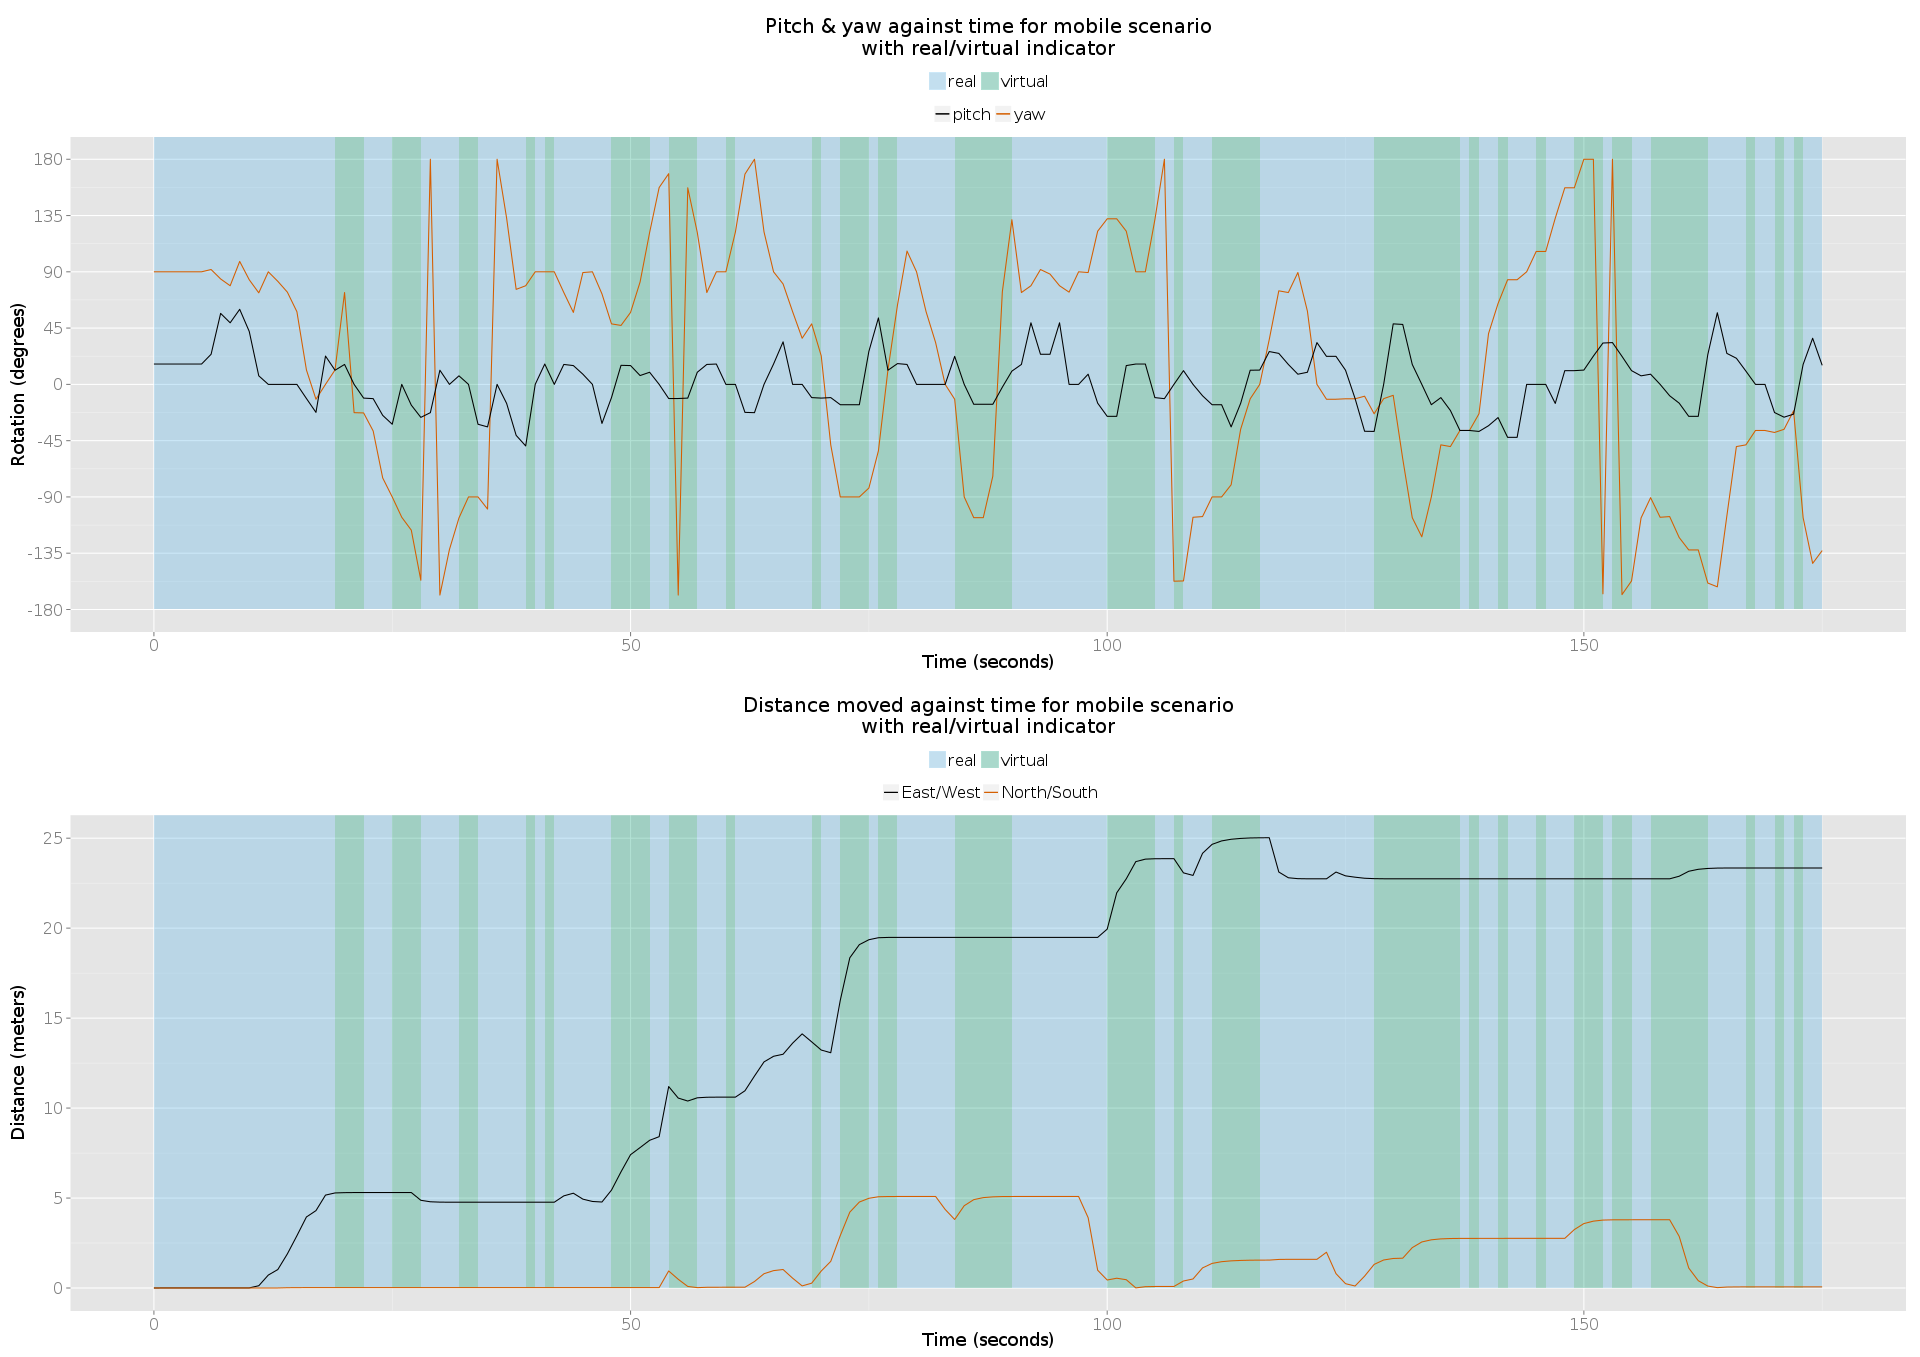
\includegraphics[width=1.2\textwidth]{1/6_2up.png}}
	\caption{Some images, yah.}
\end{figure}

%=========================================================================================================

\clearpage

\section{Phase 2.1 Results}

\lipsum[1]

\lipsum[2]

\lipsum[3]

%=========================================================================================================

\clearpage

\subsection{Participant 7}

\begin{figure}[h]
	\makebox[\textwidth][c]{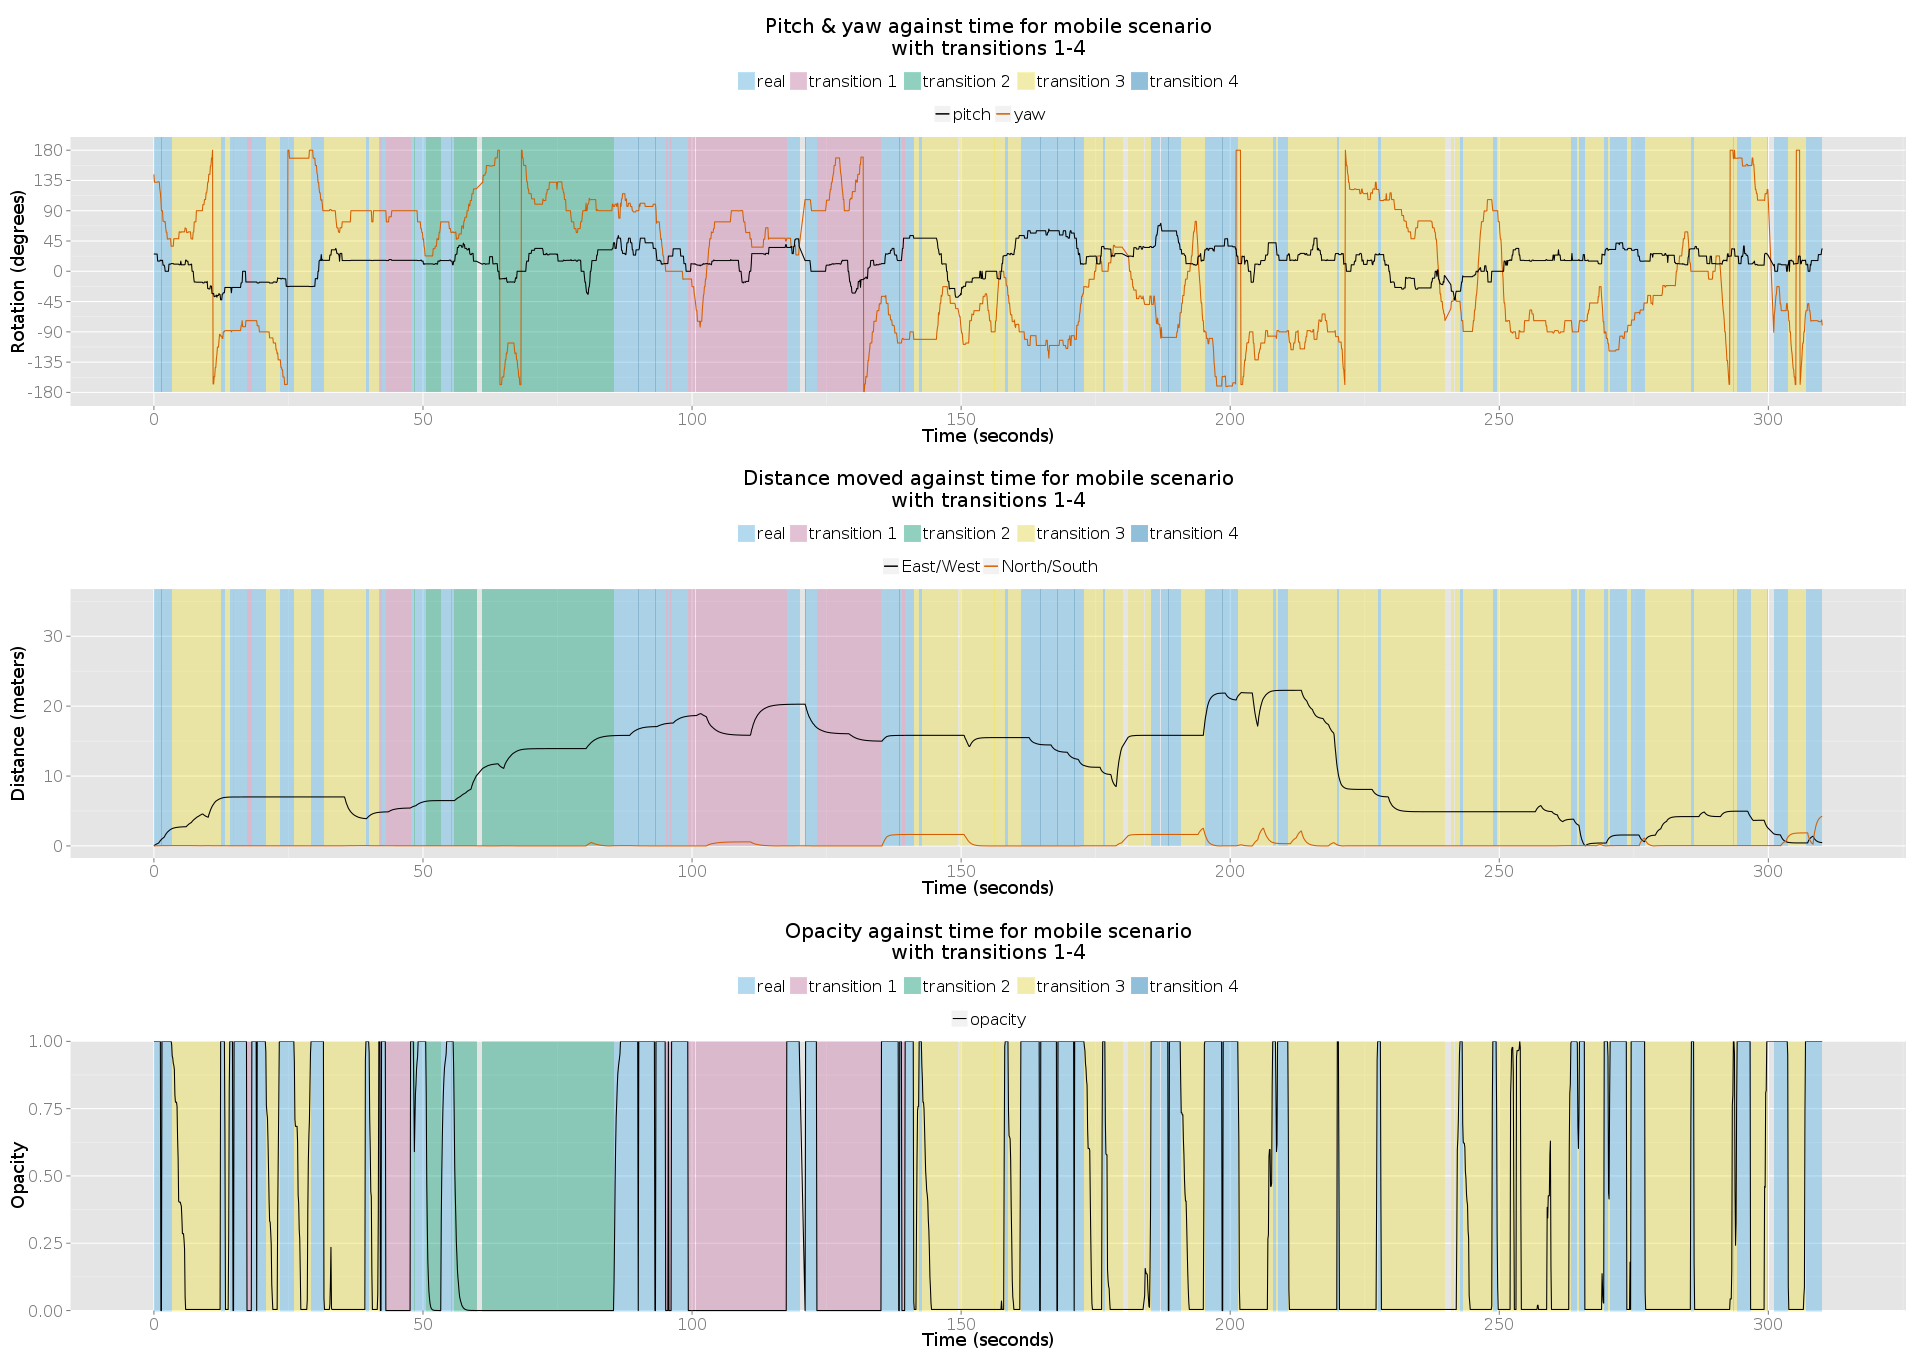
\includegraphics[width=1.2\textwidth]{2.1/7_1-4_3up.png}}
	\caption{Some images, yah.}
\end{figure}

%=========================================================================================================

\clearpage

\subsection{Participant 8}

\begin{figure}[h]
	\makebox[\textwidth][c]{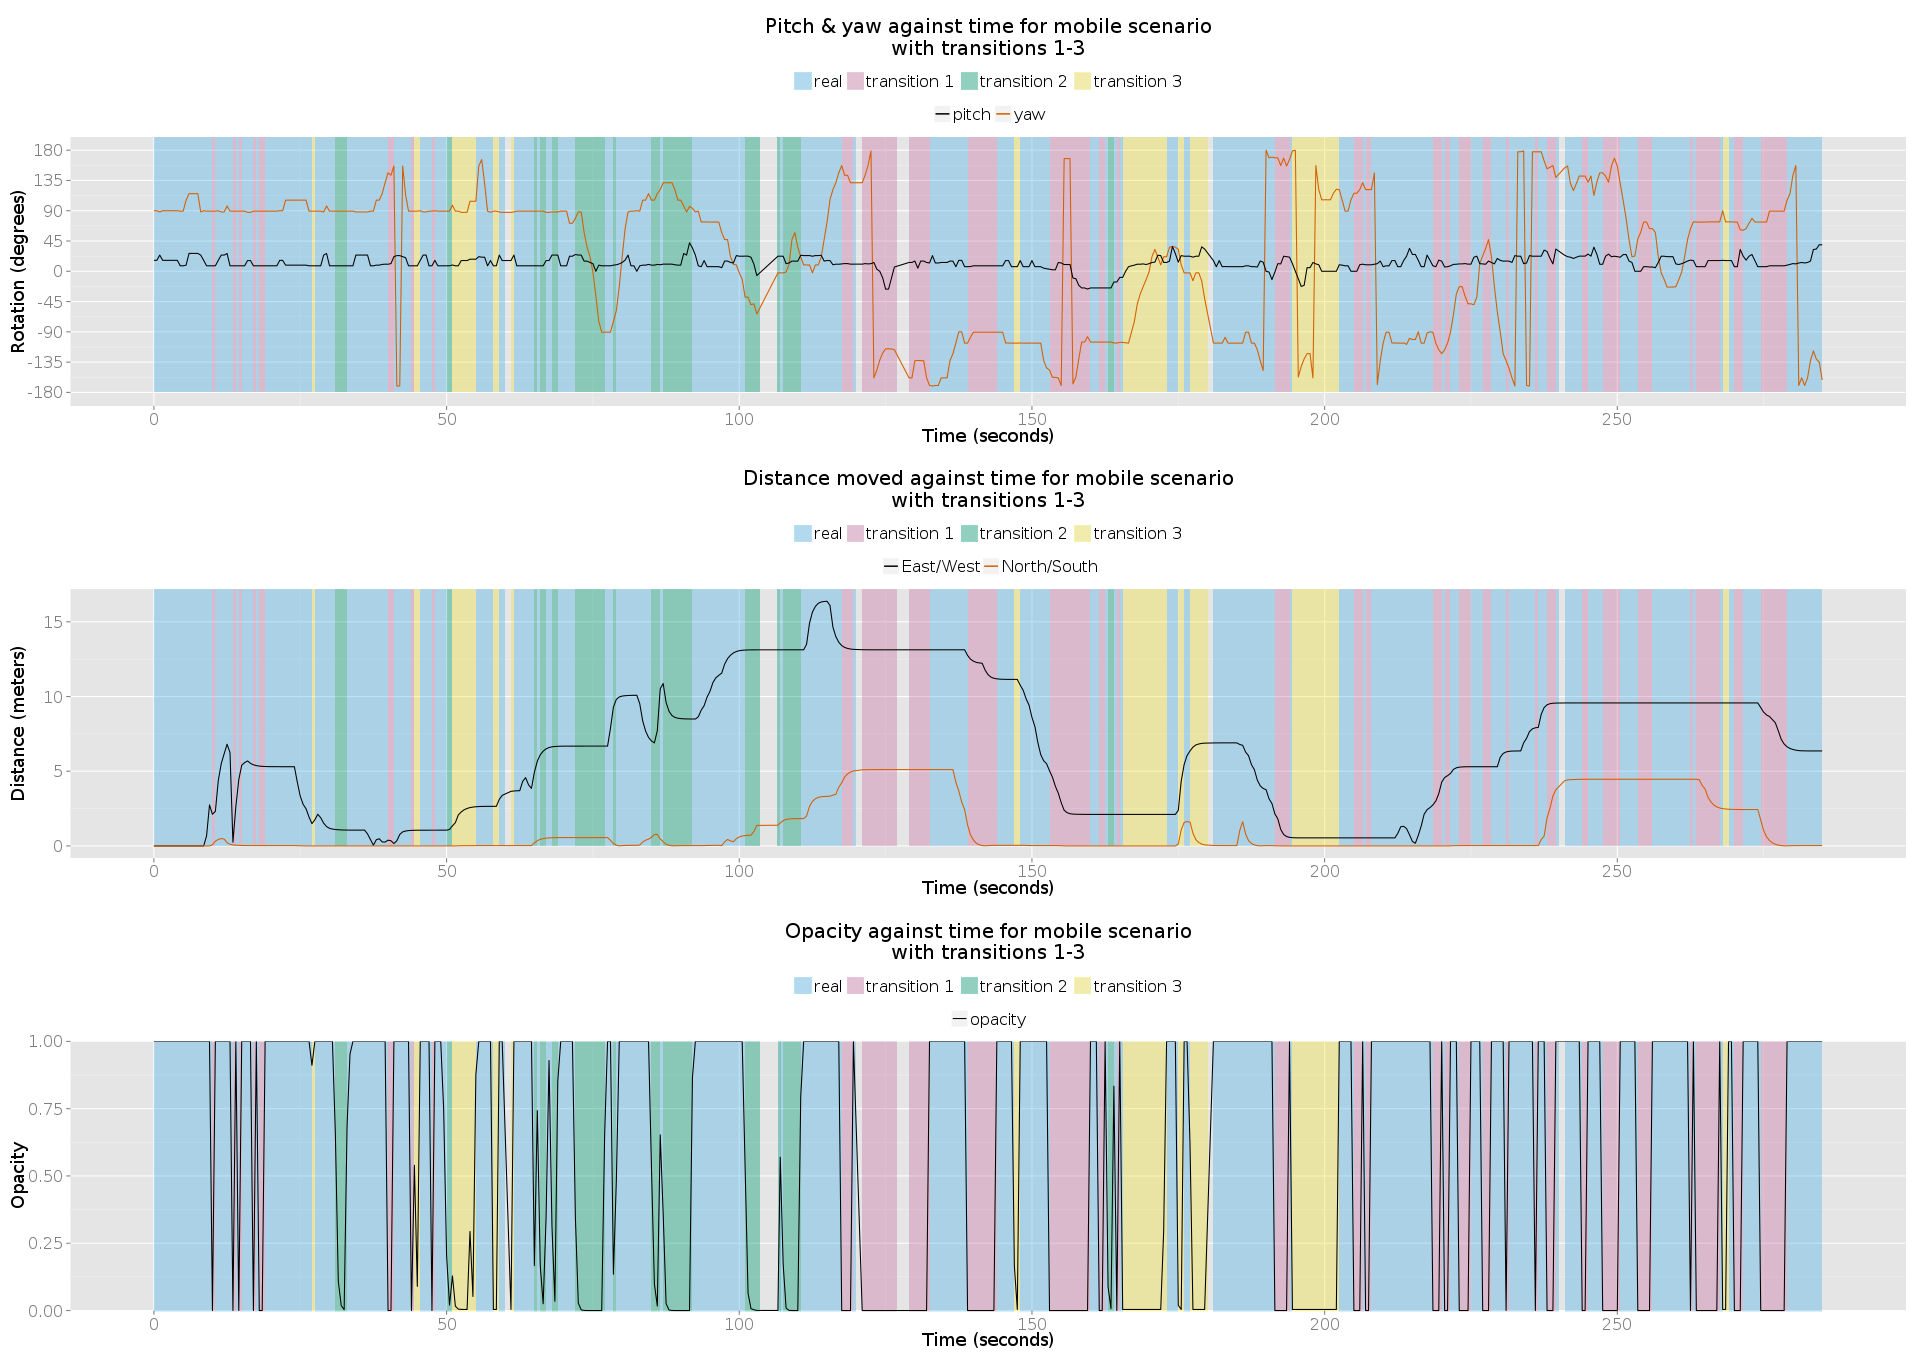
\includegraphics[width=1.2\textwidth]{2.1/8_1-3_3up.png}}
	\caption{Some images, yah.}
\end{figure}

\clearpage

\begin{figure}[h]
	\makebox[\textwidth][c]{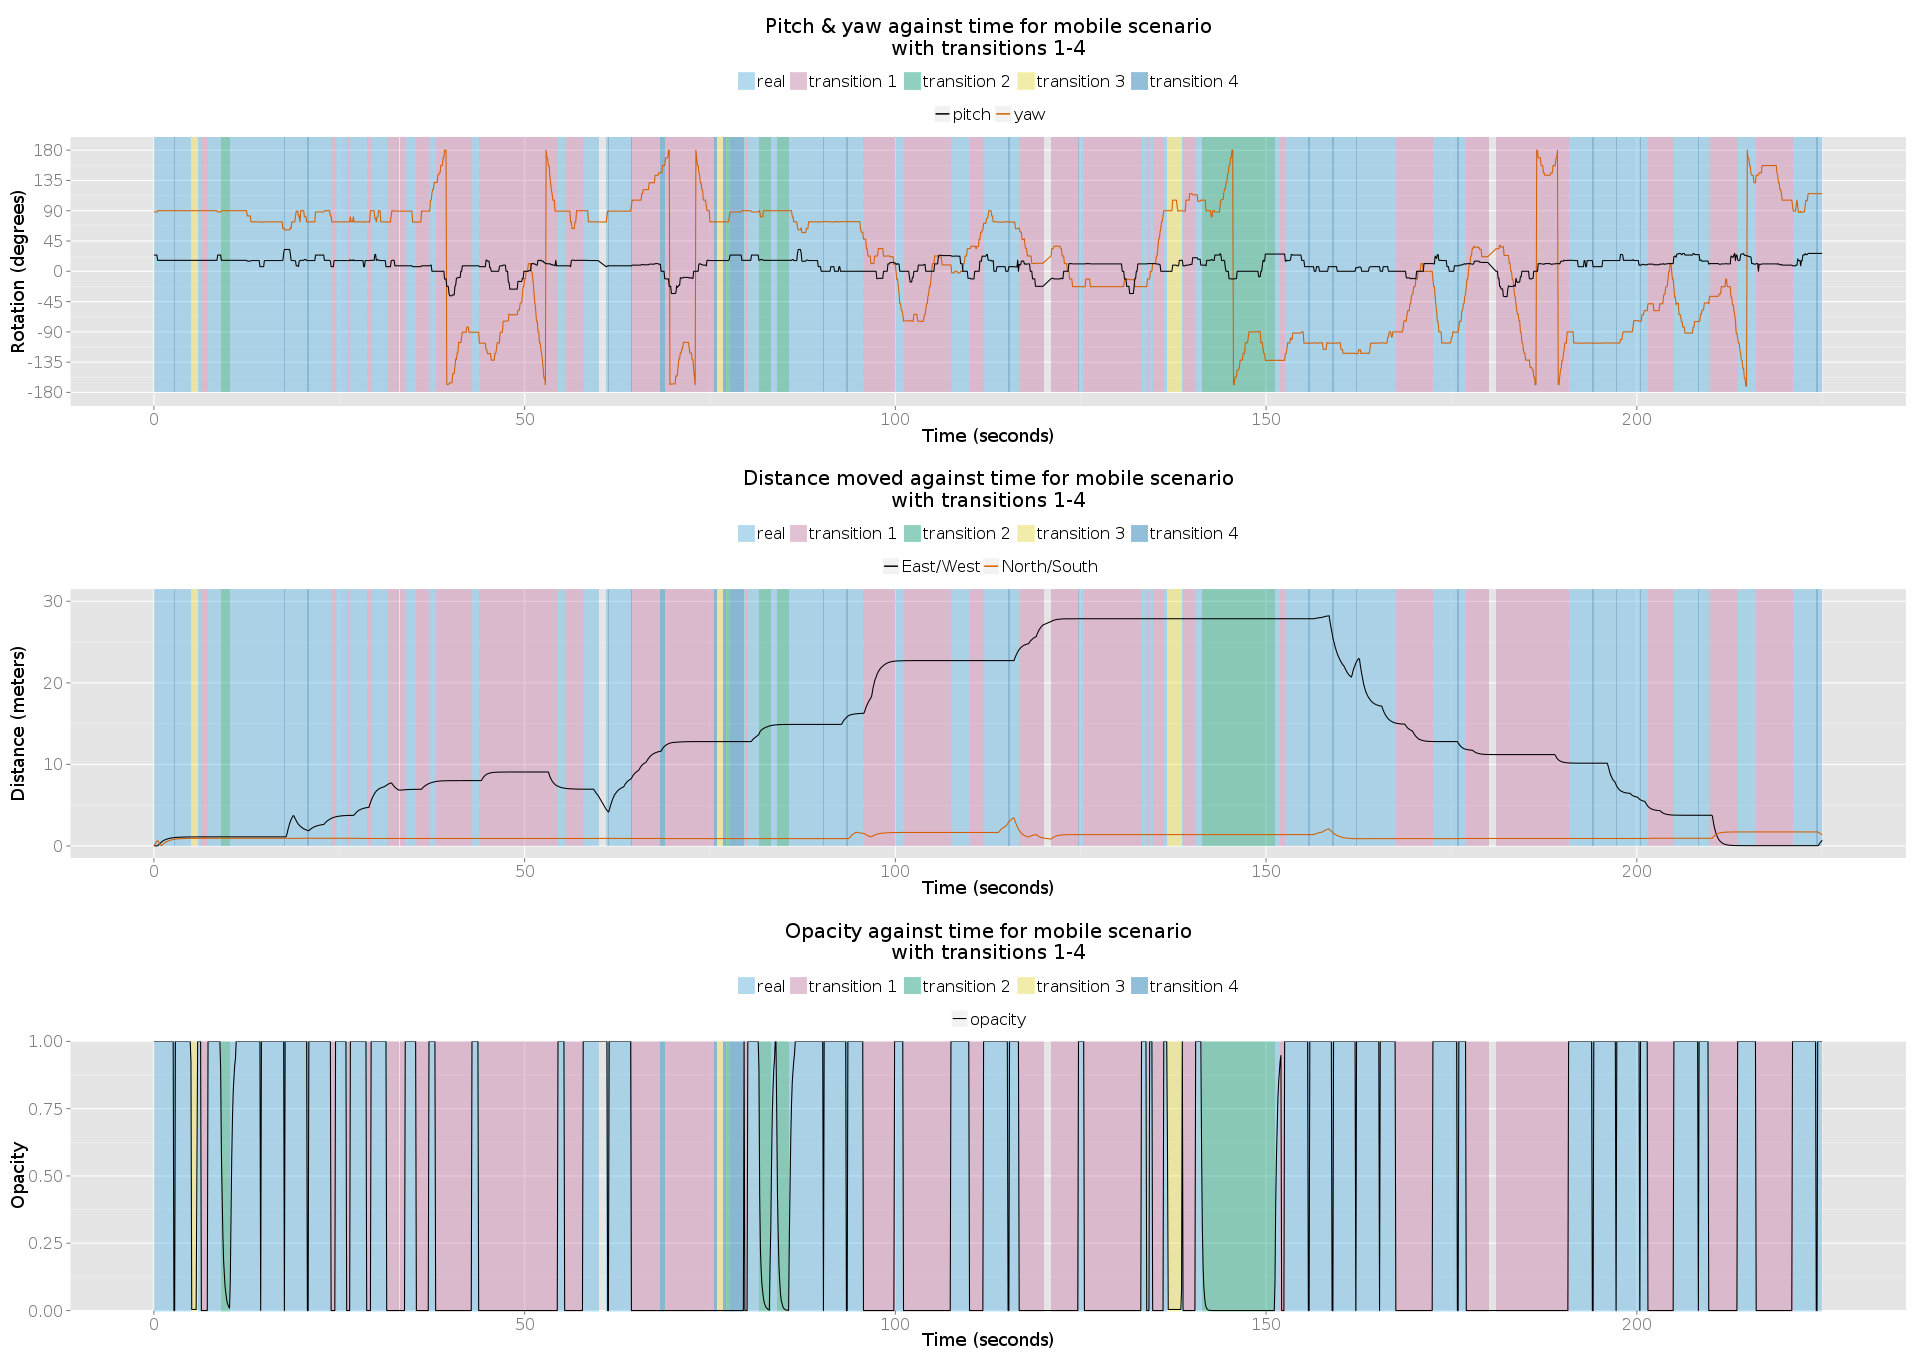
\includegraphics[width=1.2\textwidth]{2.1/8_1-4_3up.png}}
	\caption{Some images, yah.}
\end{figure}

%=========================================================================================================

\clearpage

\subsection{Participant 9}

\begin{figure}[h]
	\makebox[\textwidth][c]{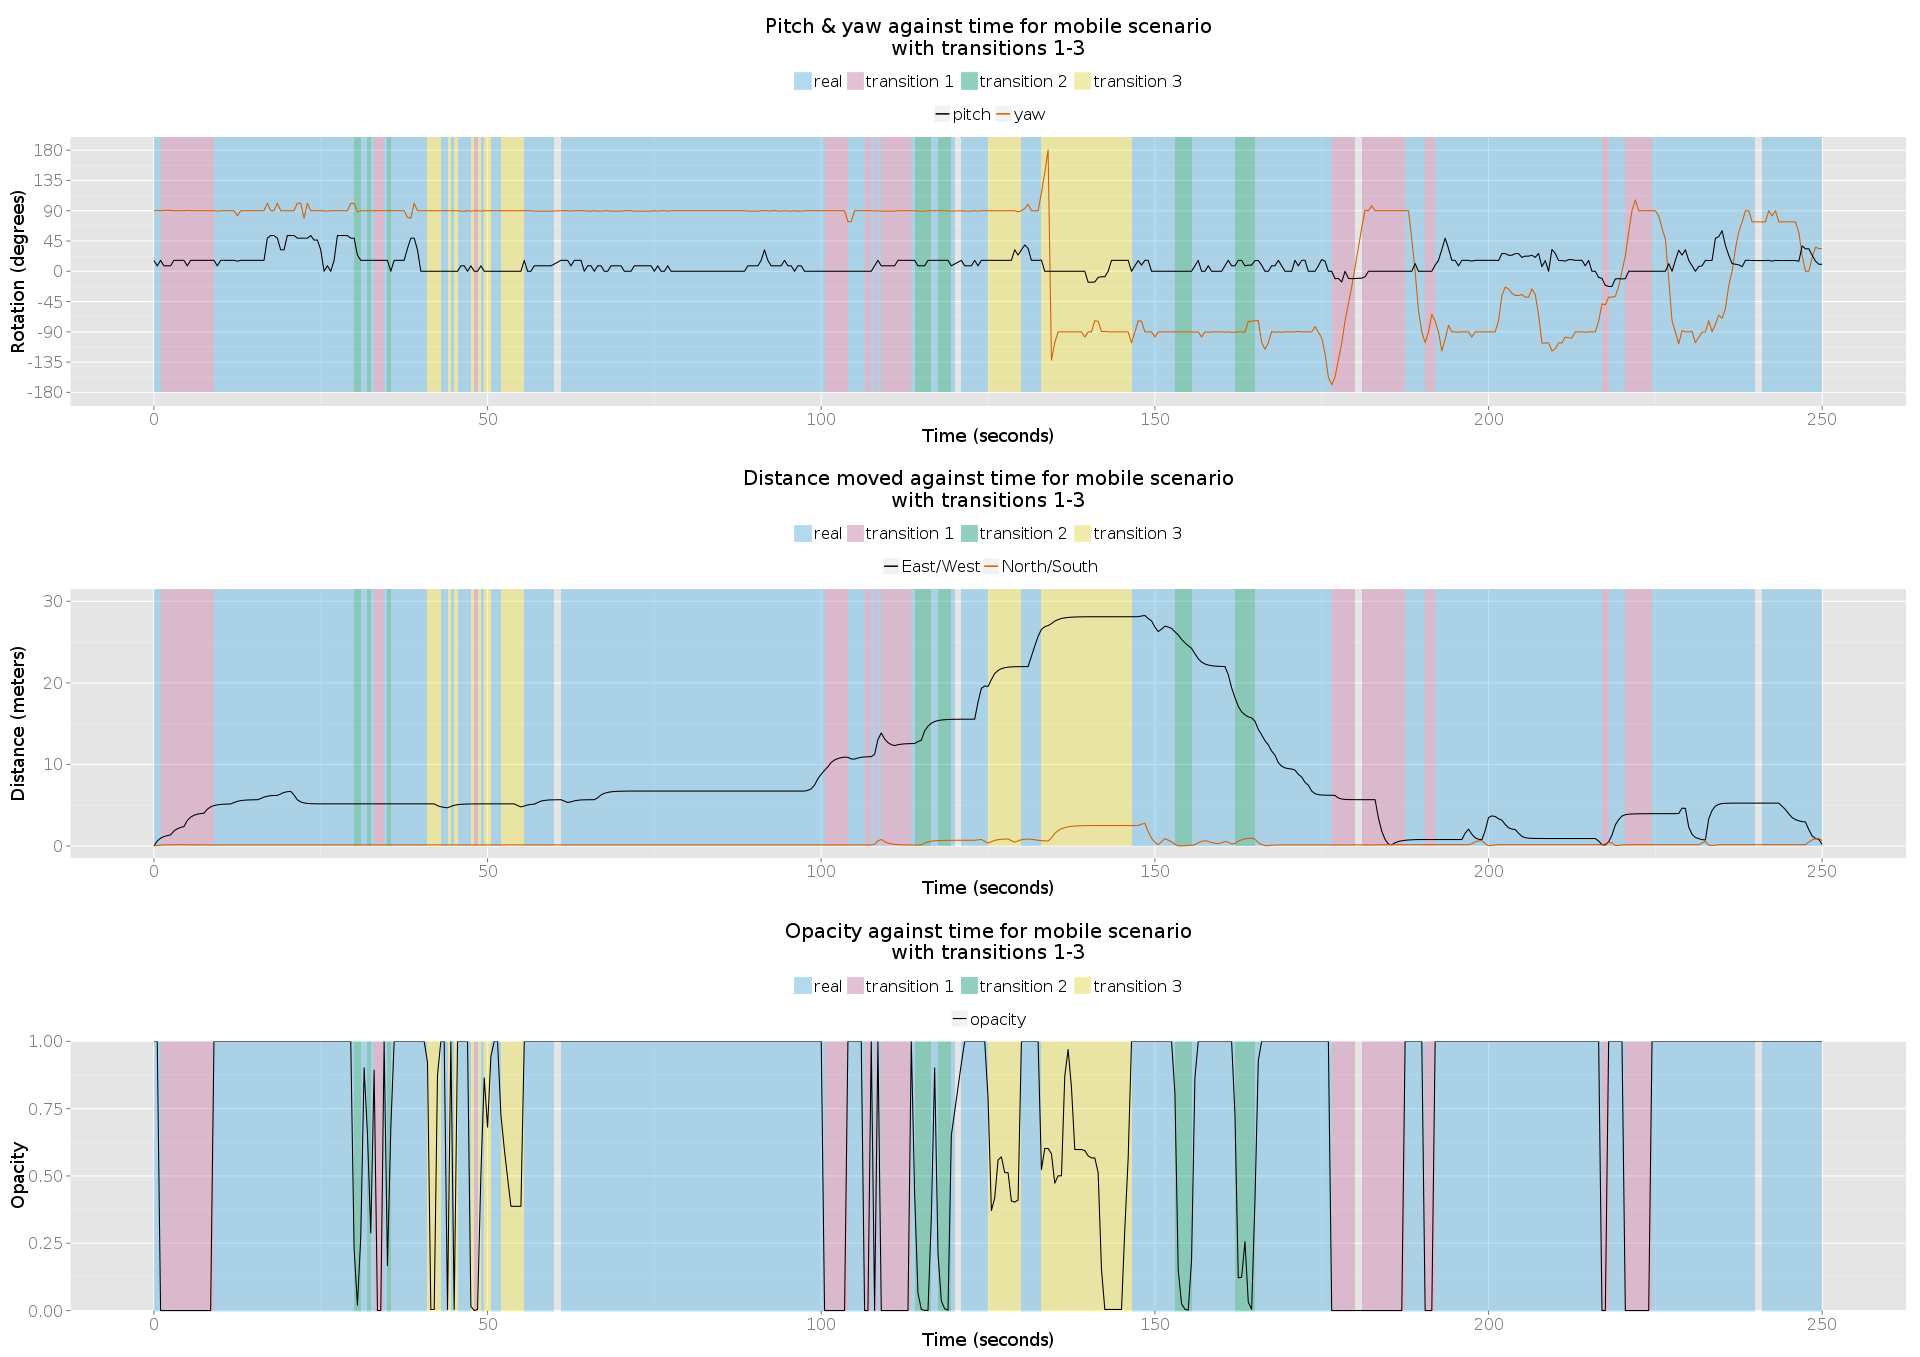
\includegraphics[width=1.2\textwidth]{2.1/9_1-3_3up.png}}
	\caption{Some images, yah.}
\end{figure}

\clearpage

\begin{figure}[h]
	\makebox[\textwidth][c]{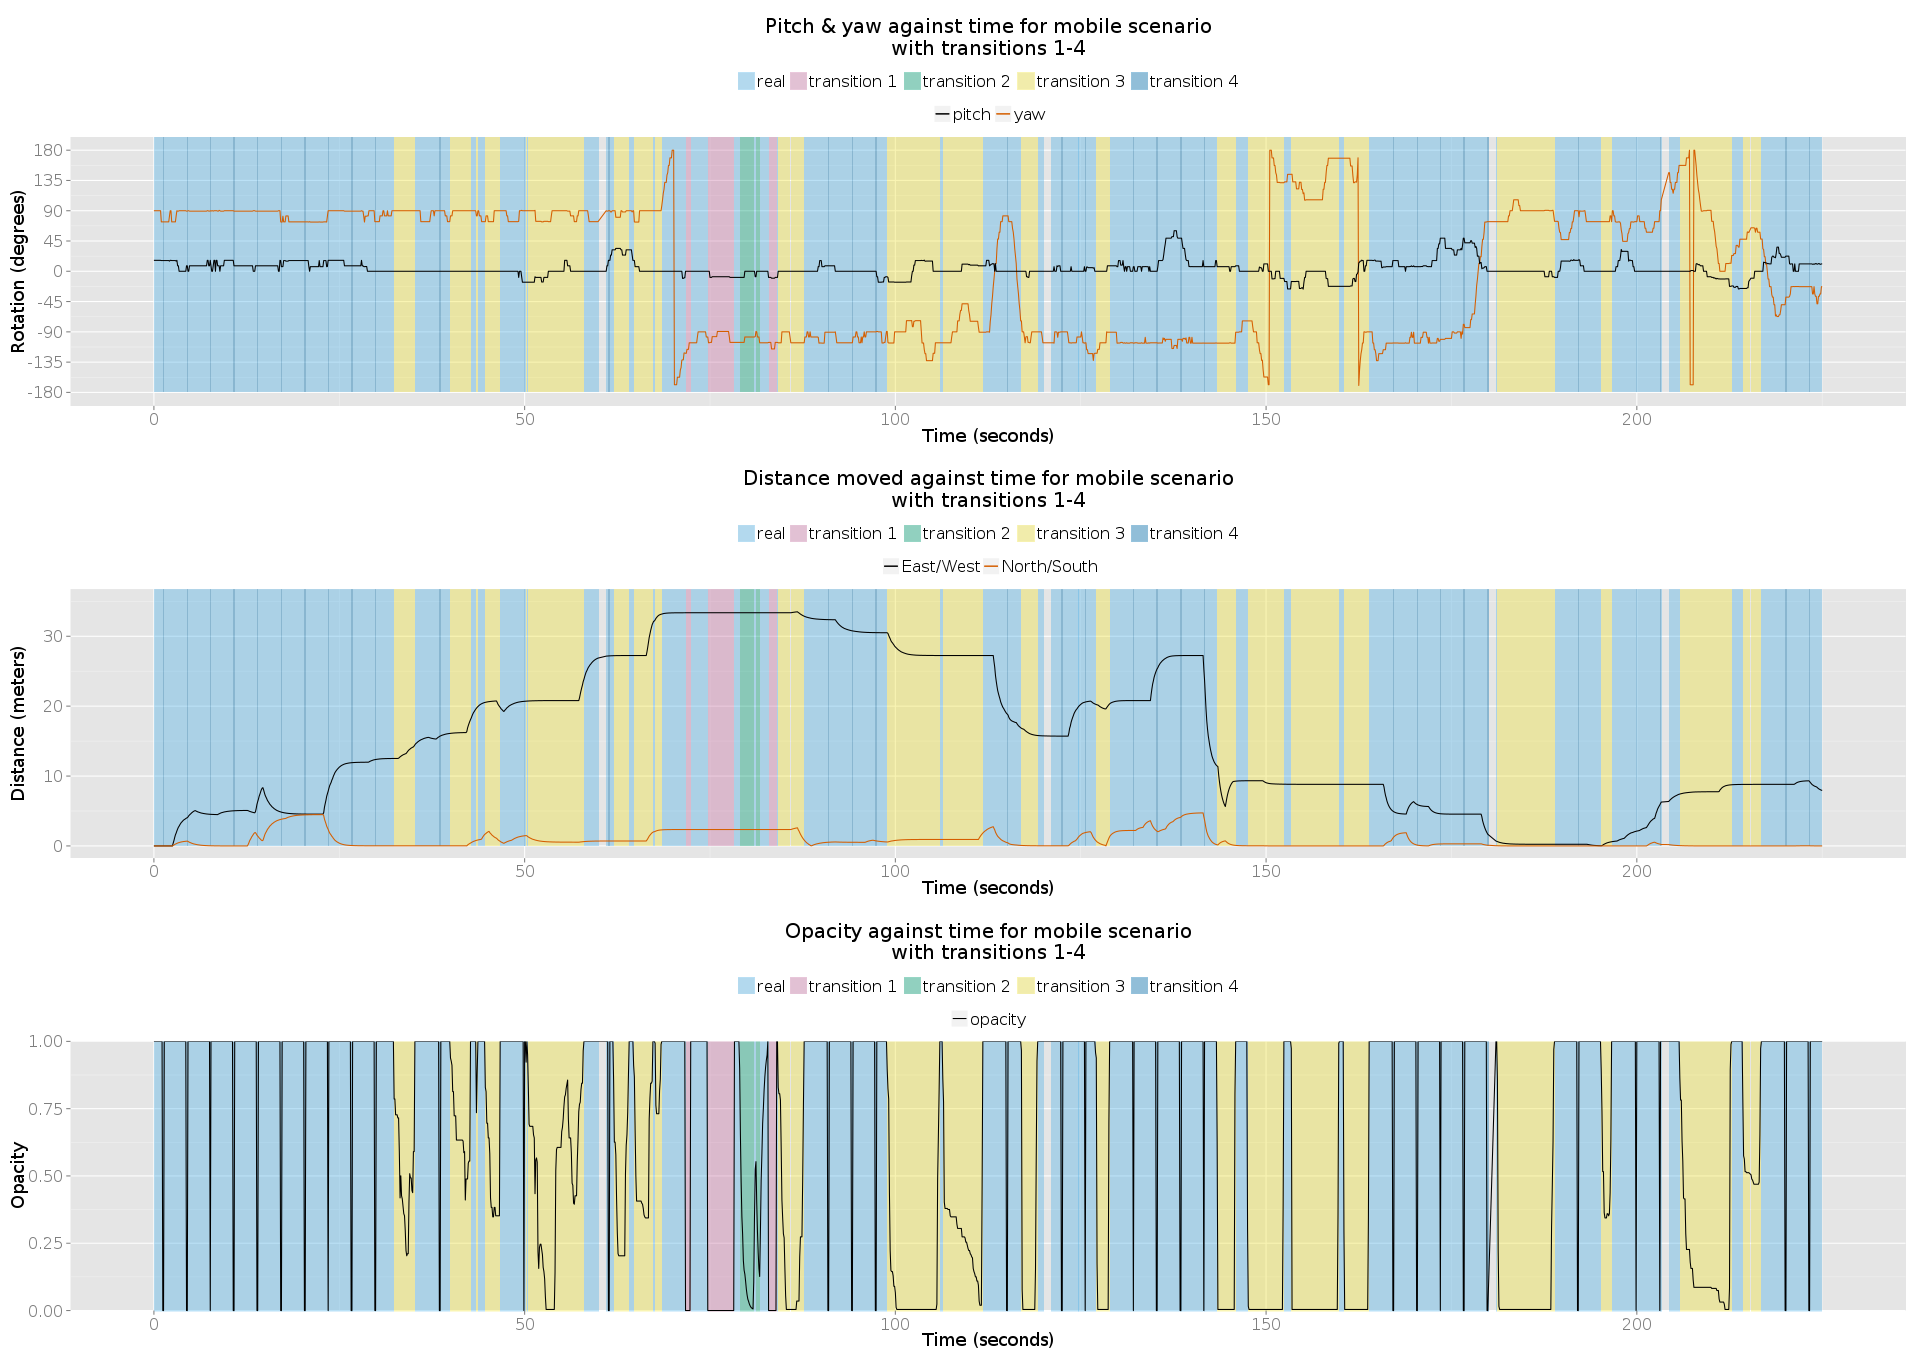
\includegraphics[width=1.2\textwidth]{2.1/9_1-4_3up.png}}
	\caption{Some images, yah.}
\end{figure}

%=========================================================================================================

\clearpage

\subsection{Participant 10}

\begin{figure}[h]
	\makebox[\textwidth][c]{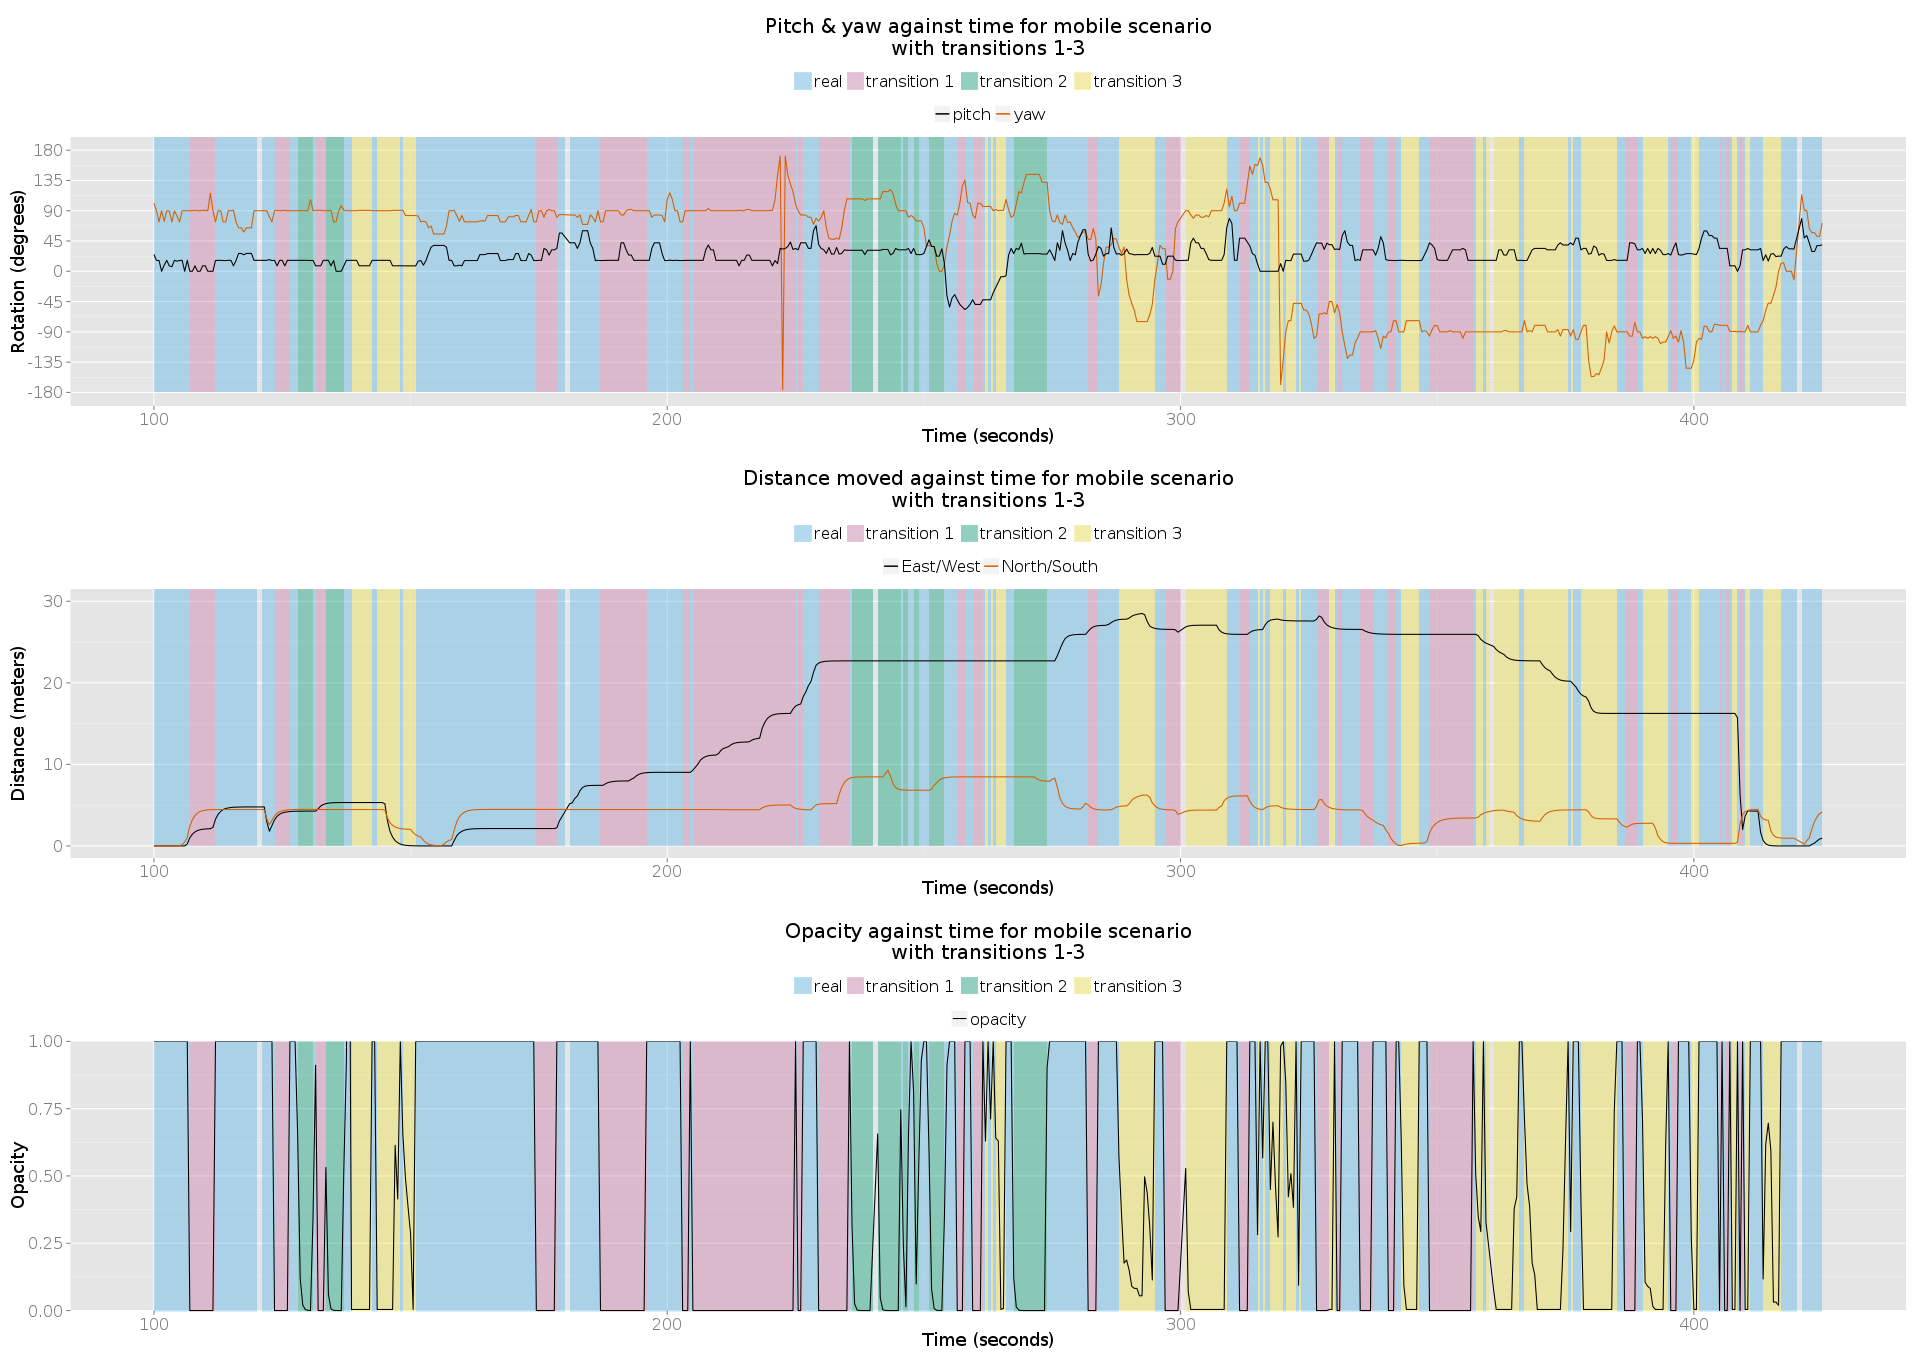
\includegraphics[width=1.2\textwidth]{2.1/10_1-3_3up.png}}
	\caption{Some images, yah.}
\end{figure}

\clearpage

\begin{figure}[h]
	\makebox[\textwidth][c]{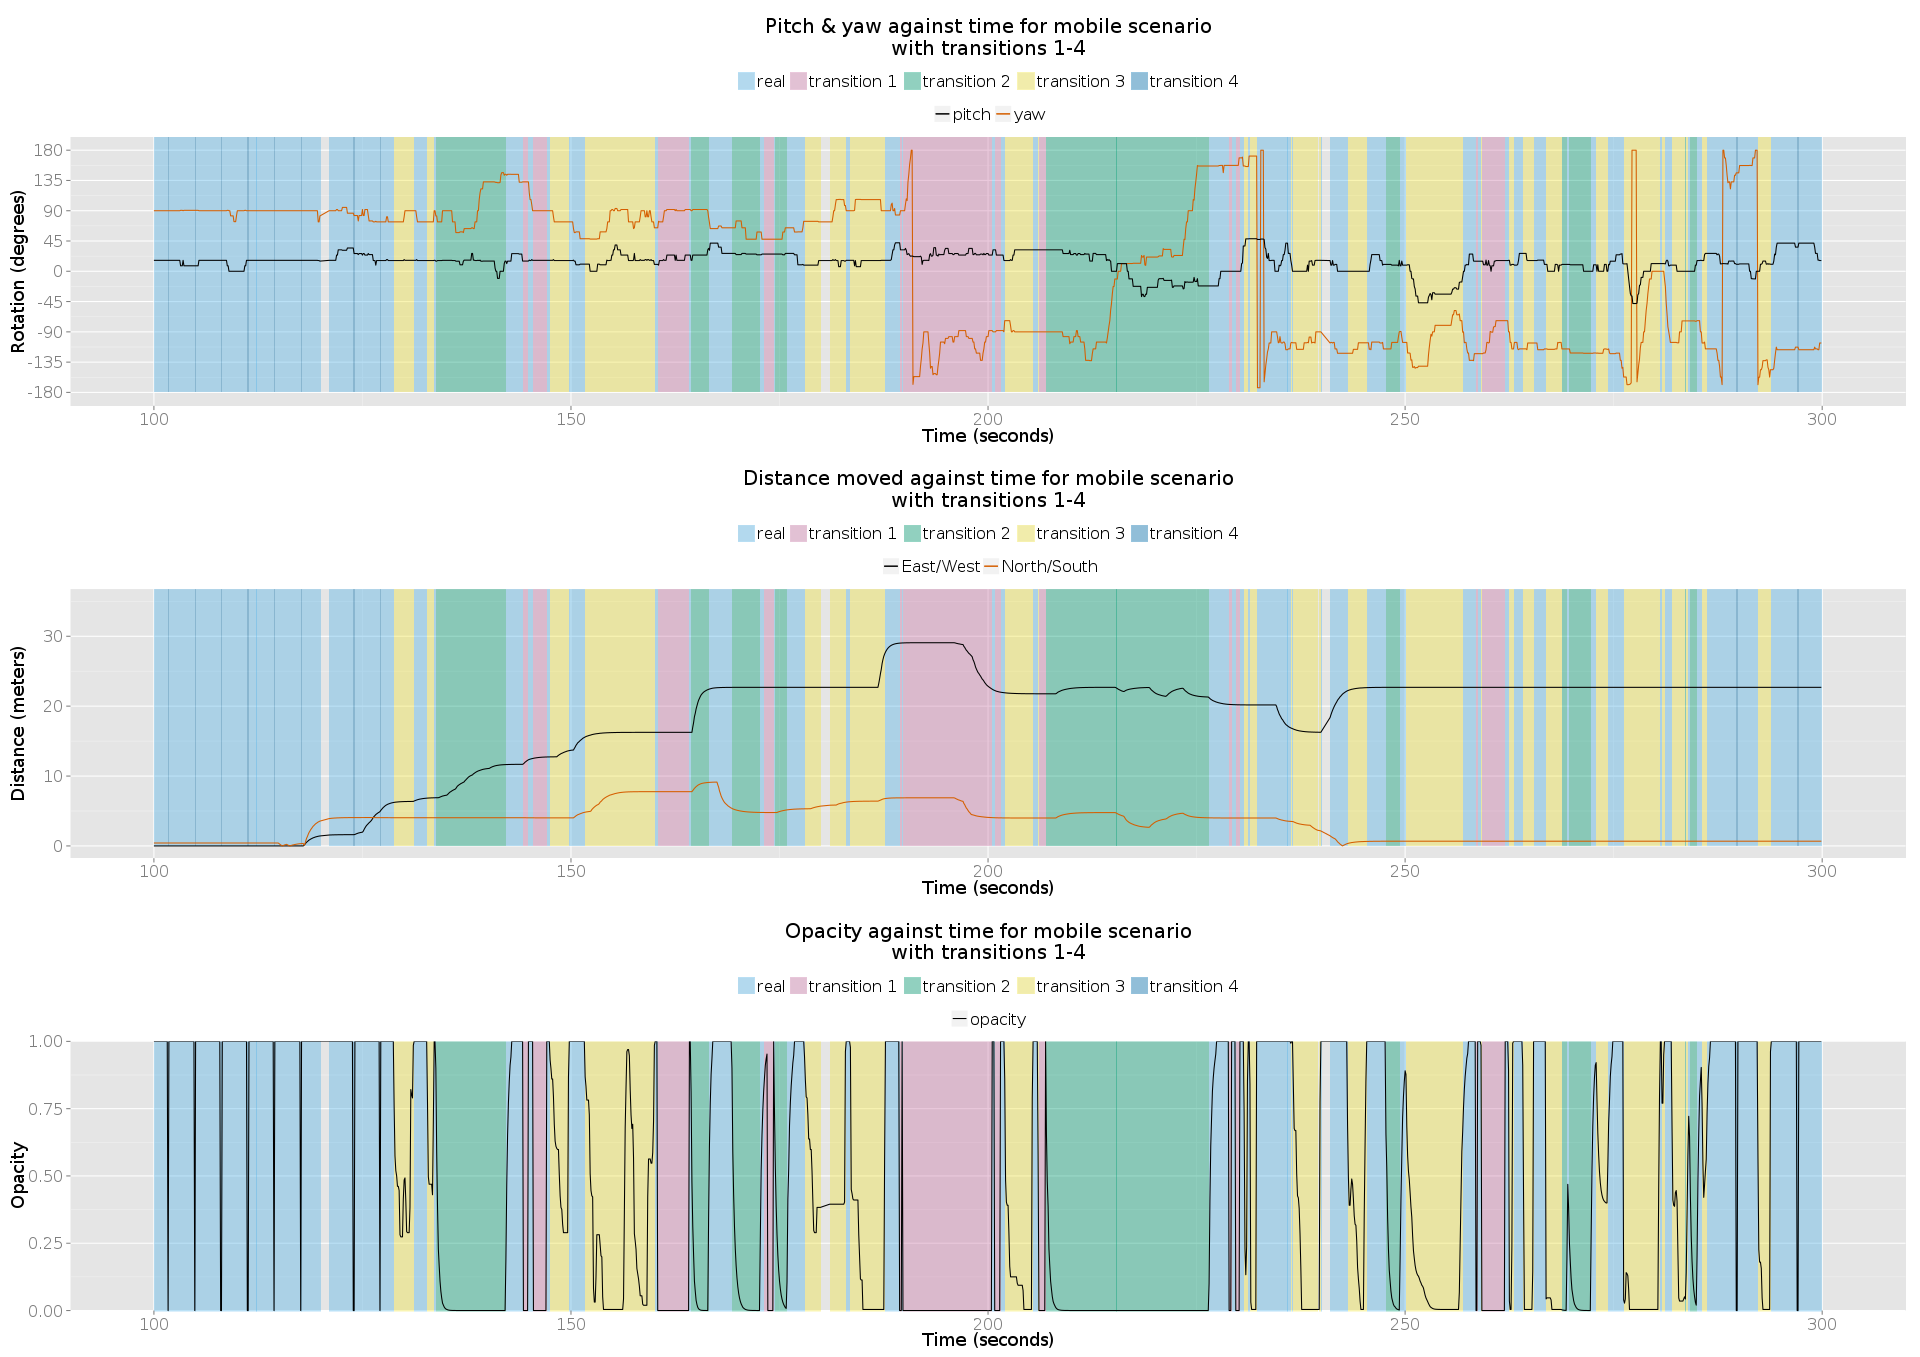
\includegraphics[width=1.2\textwidth]{2.1/10_1-4_3up.png}}
	\caption{Some images, yah.}
\end{figure}

%=========================================================================================================

\clearpage

\subsection{Participant 11}

\begin{figure}[h]
	\makebox[\textwidth][c]{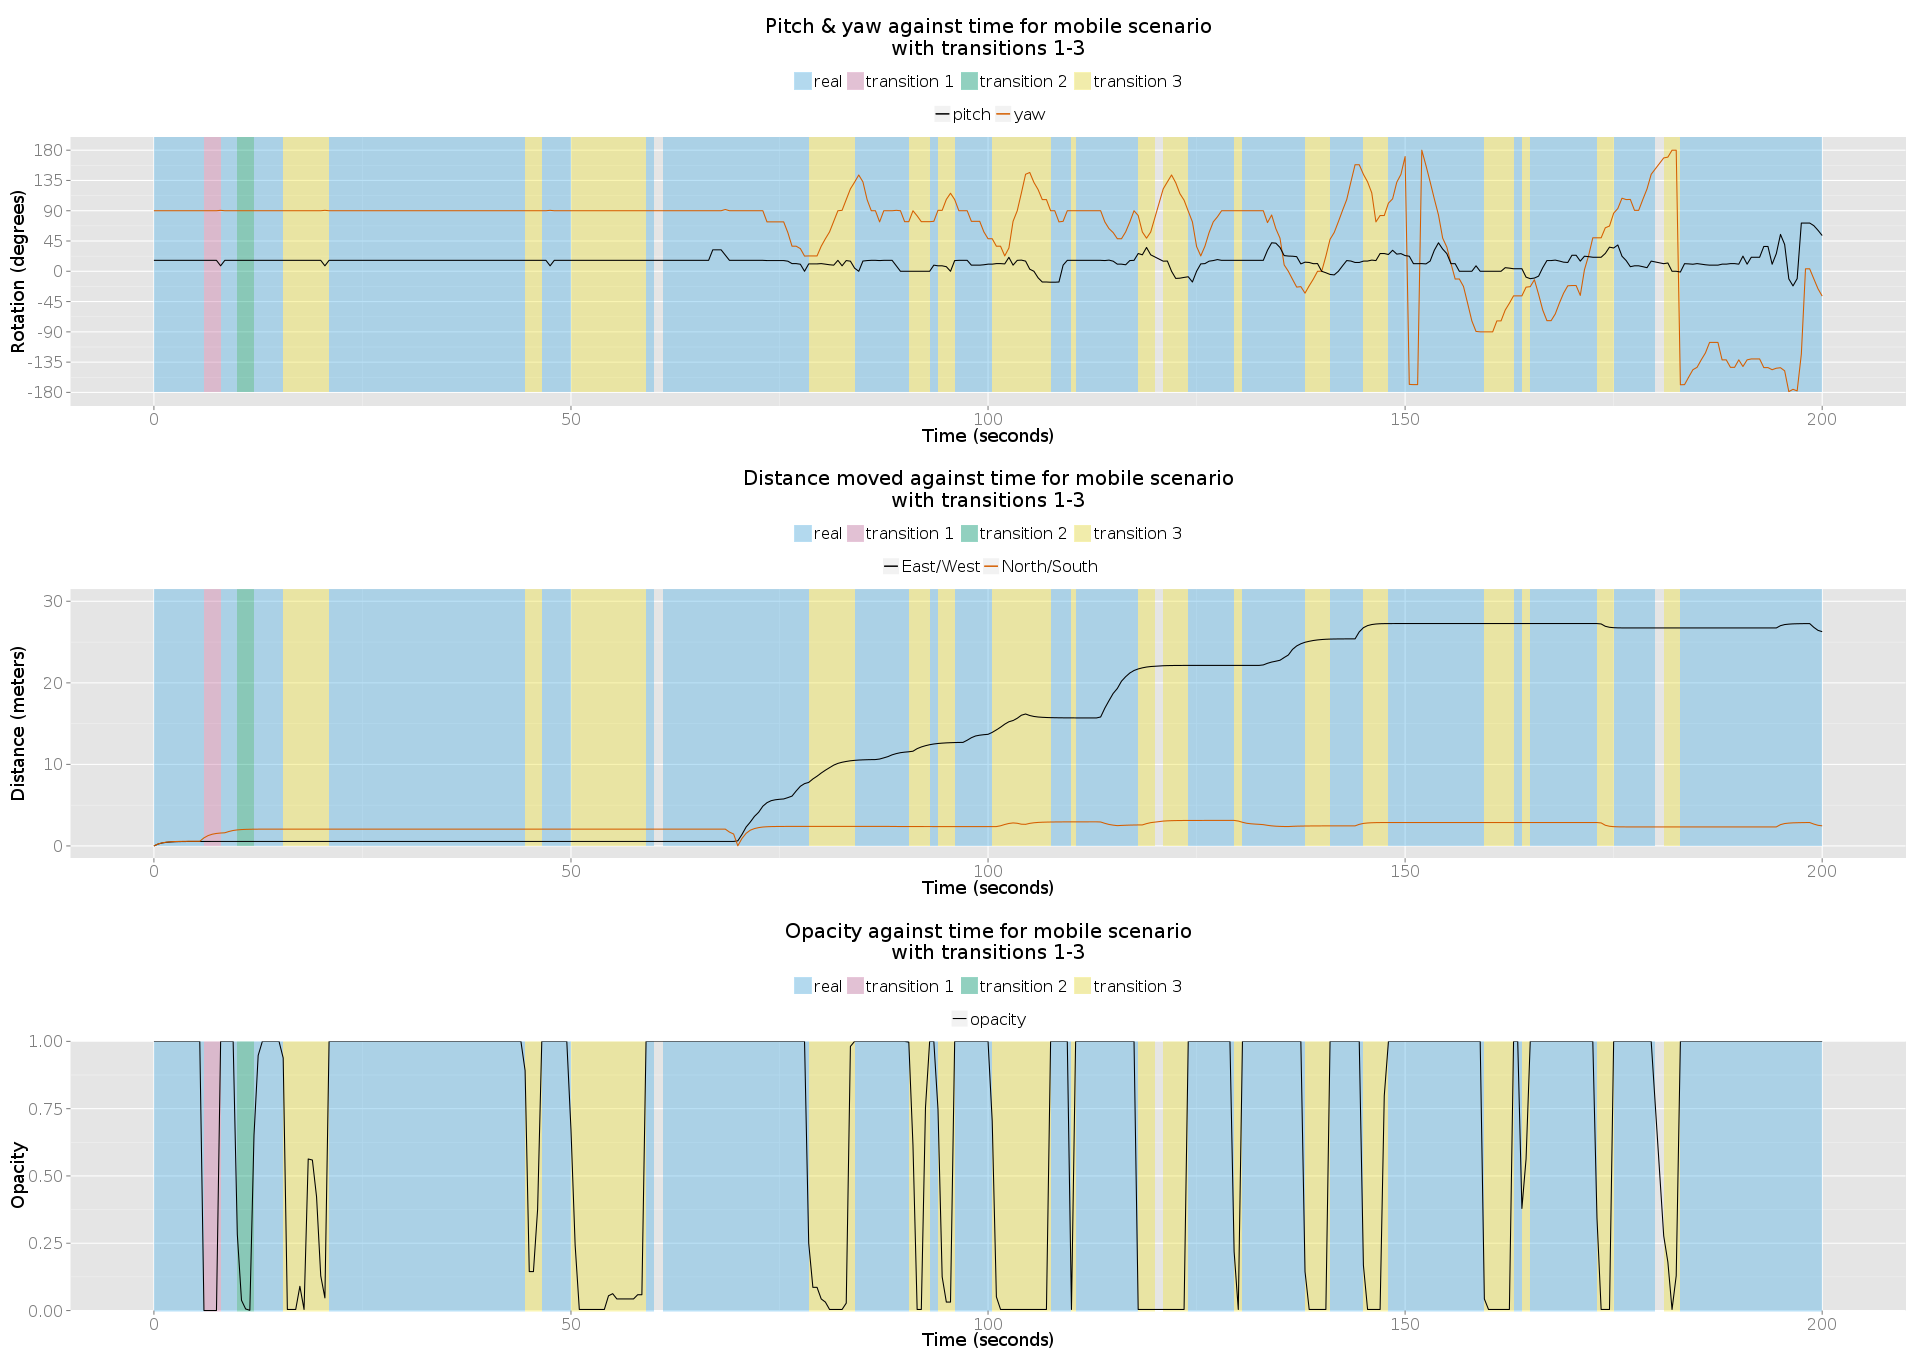
\includegraphics[width=1.2\textwidth]{2.1/11_1-3_3up.png}}
	\caption{Some images, yah.}
\end{figure}

\clearpage

\begin{figure}[h]
	\makebox[\textwidth][c]{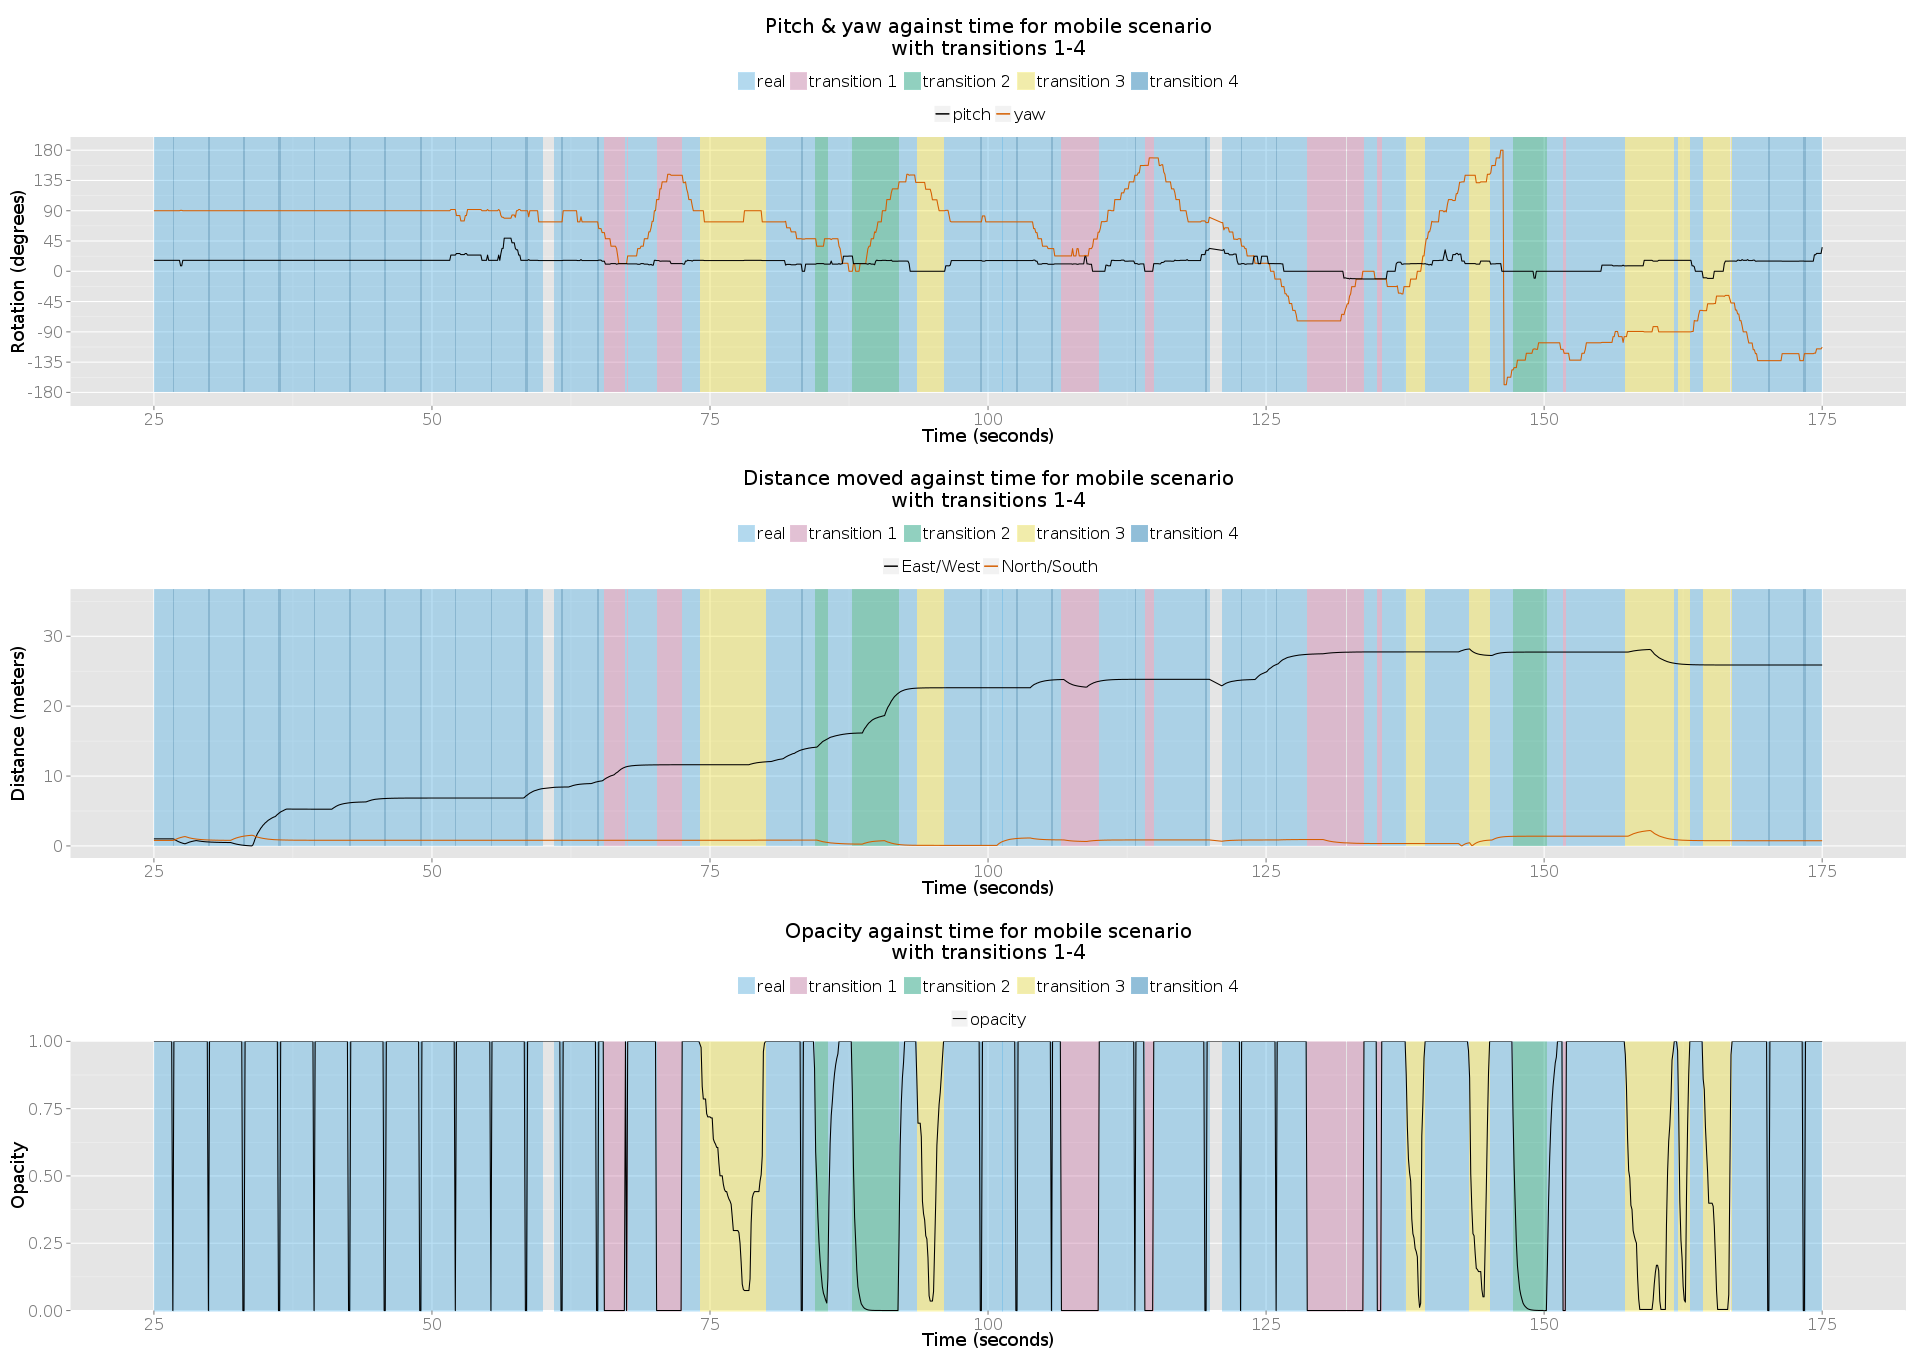
\includegraphics[width=1.2\textwidth]{2.1/11_1-4_3up.png}}
	\caption{Some images, yah.}
\end{figure}

%=========================================================================================================

\clearpage

\subsection{Participant 12}

\begin{figure}[h]
	\makebox[\textwidth][c]{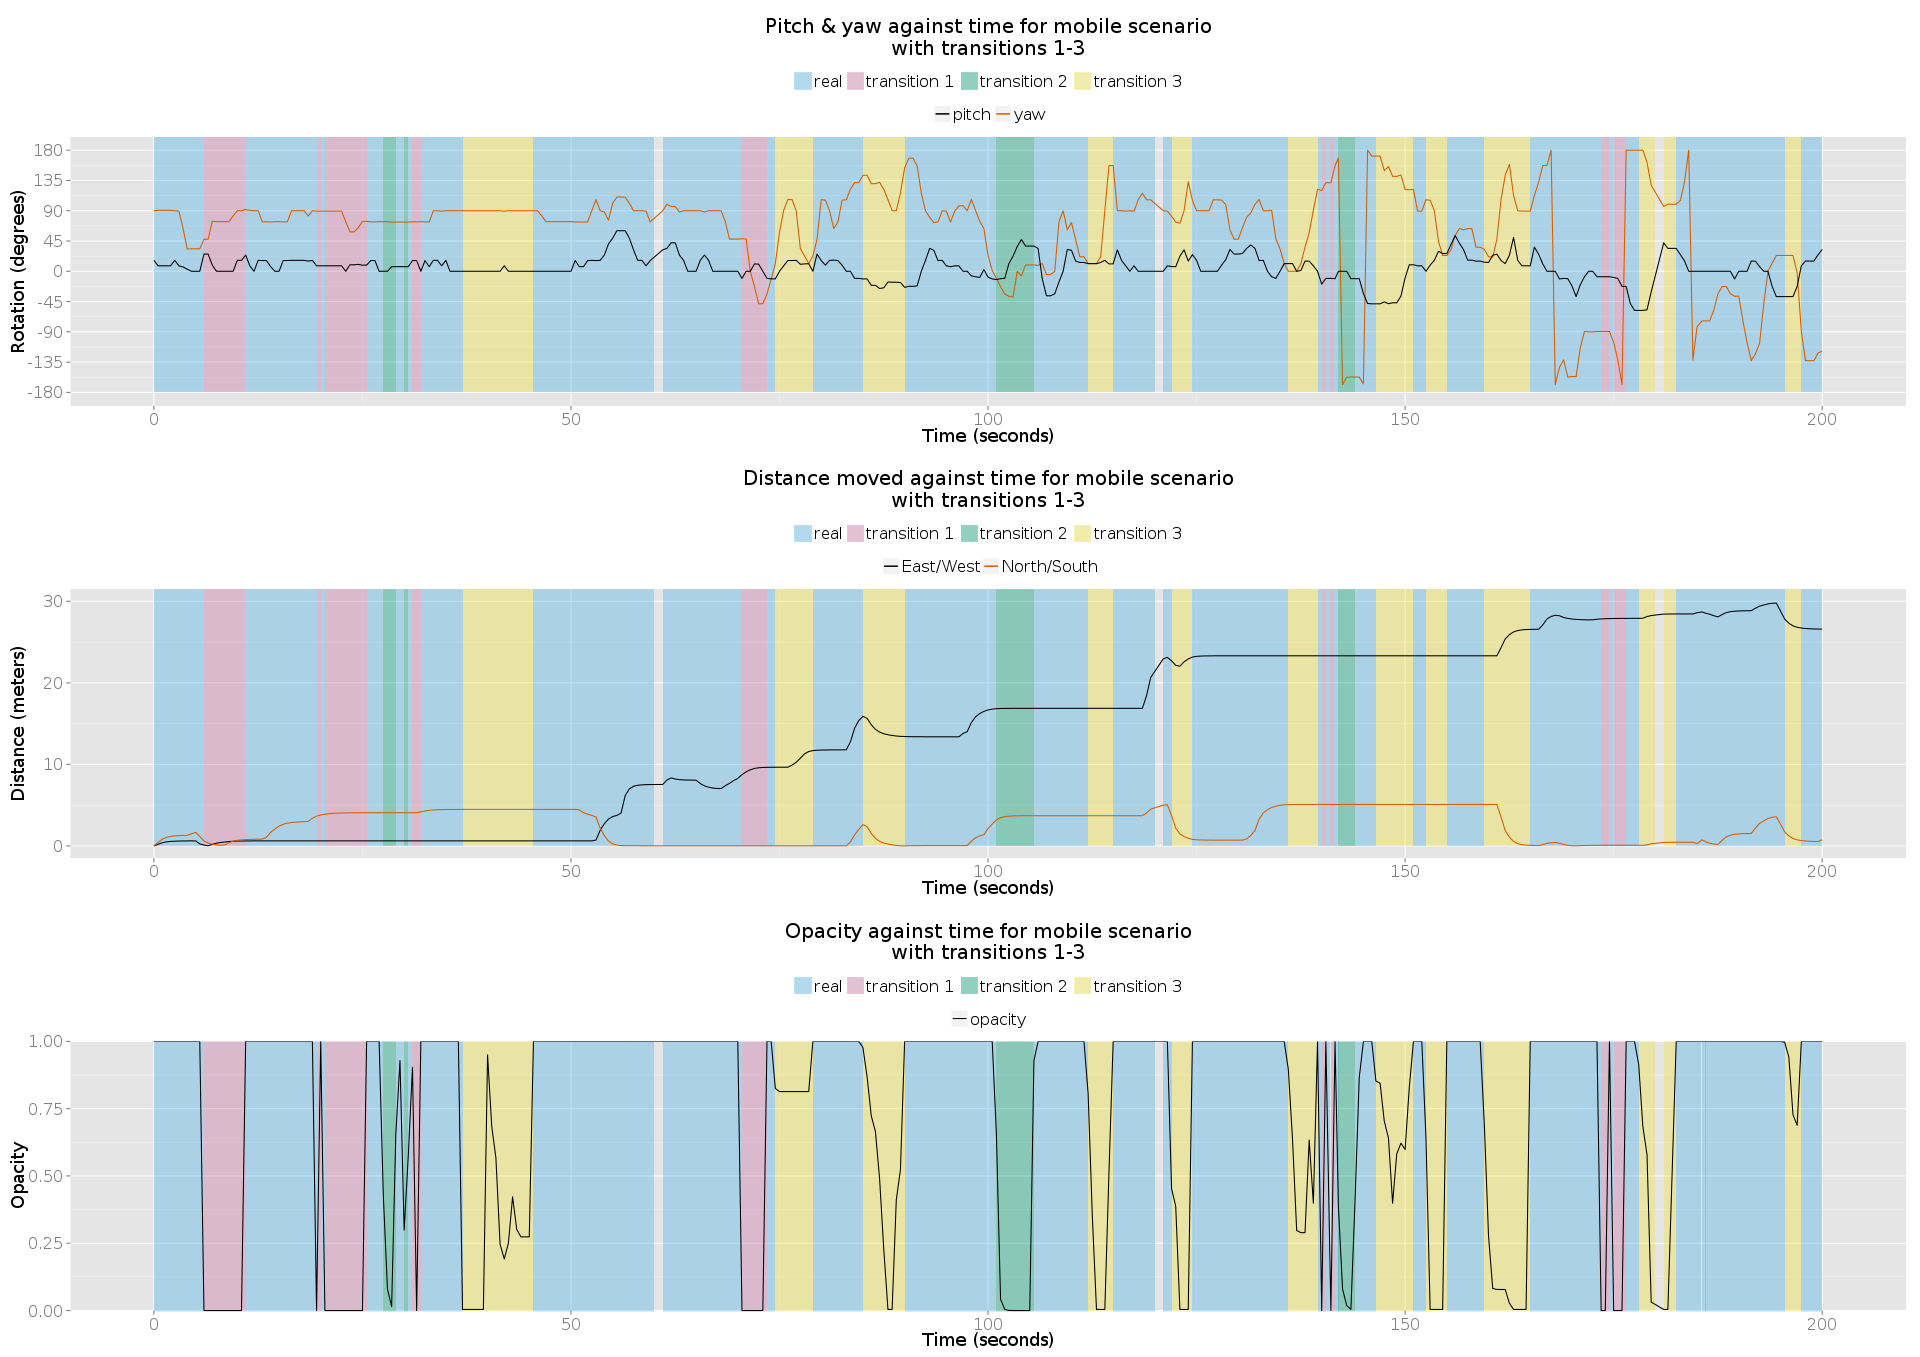
\includegraphics[width=1.2\textwidth]{2.1/12_1-3_3up.png}}
	\caption{Some images, yah.}
\end{figure}

\clearpage

\begin{figure}[h]
	\makebox[\textwidth][c]{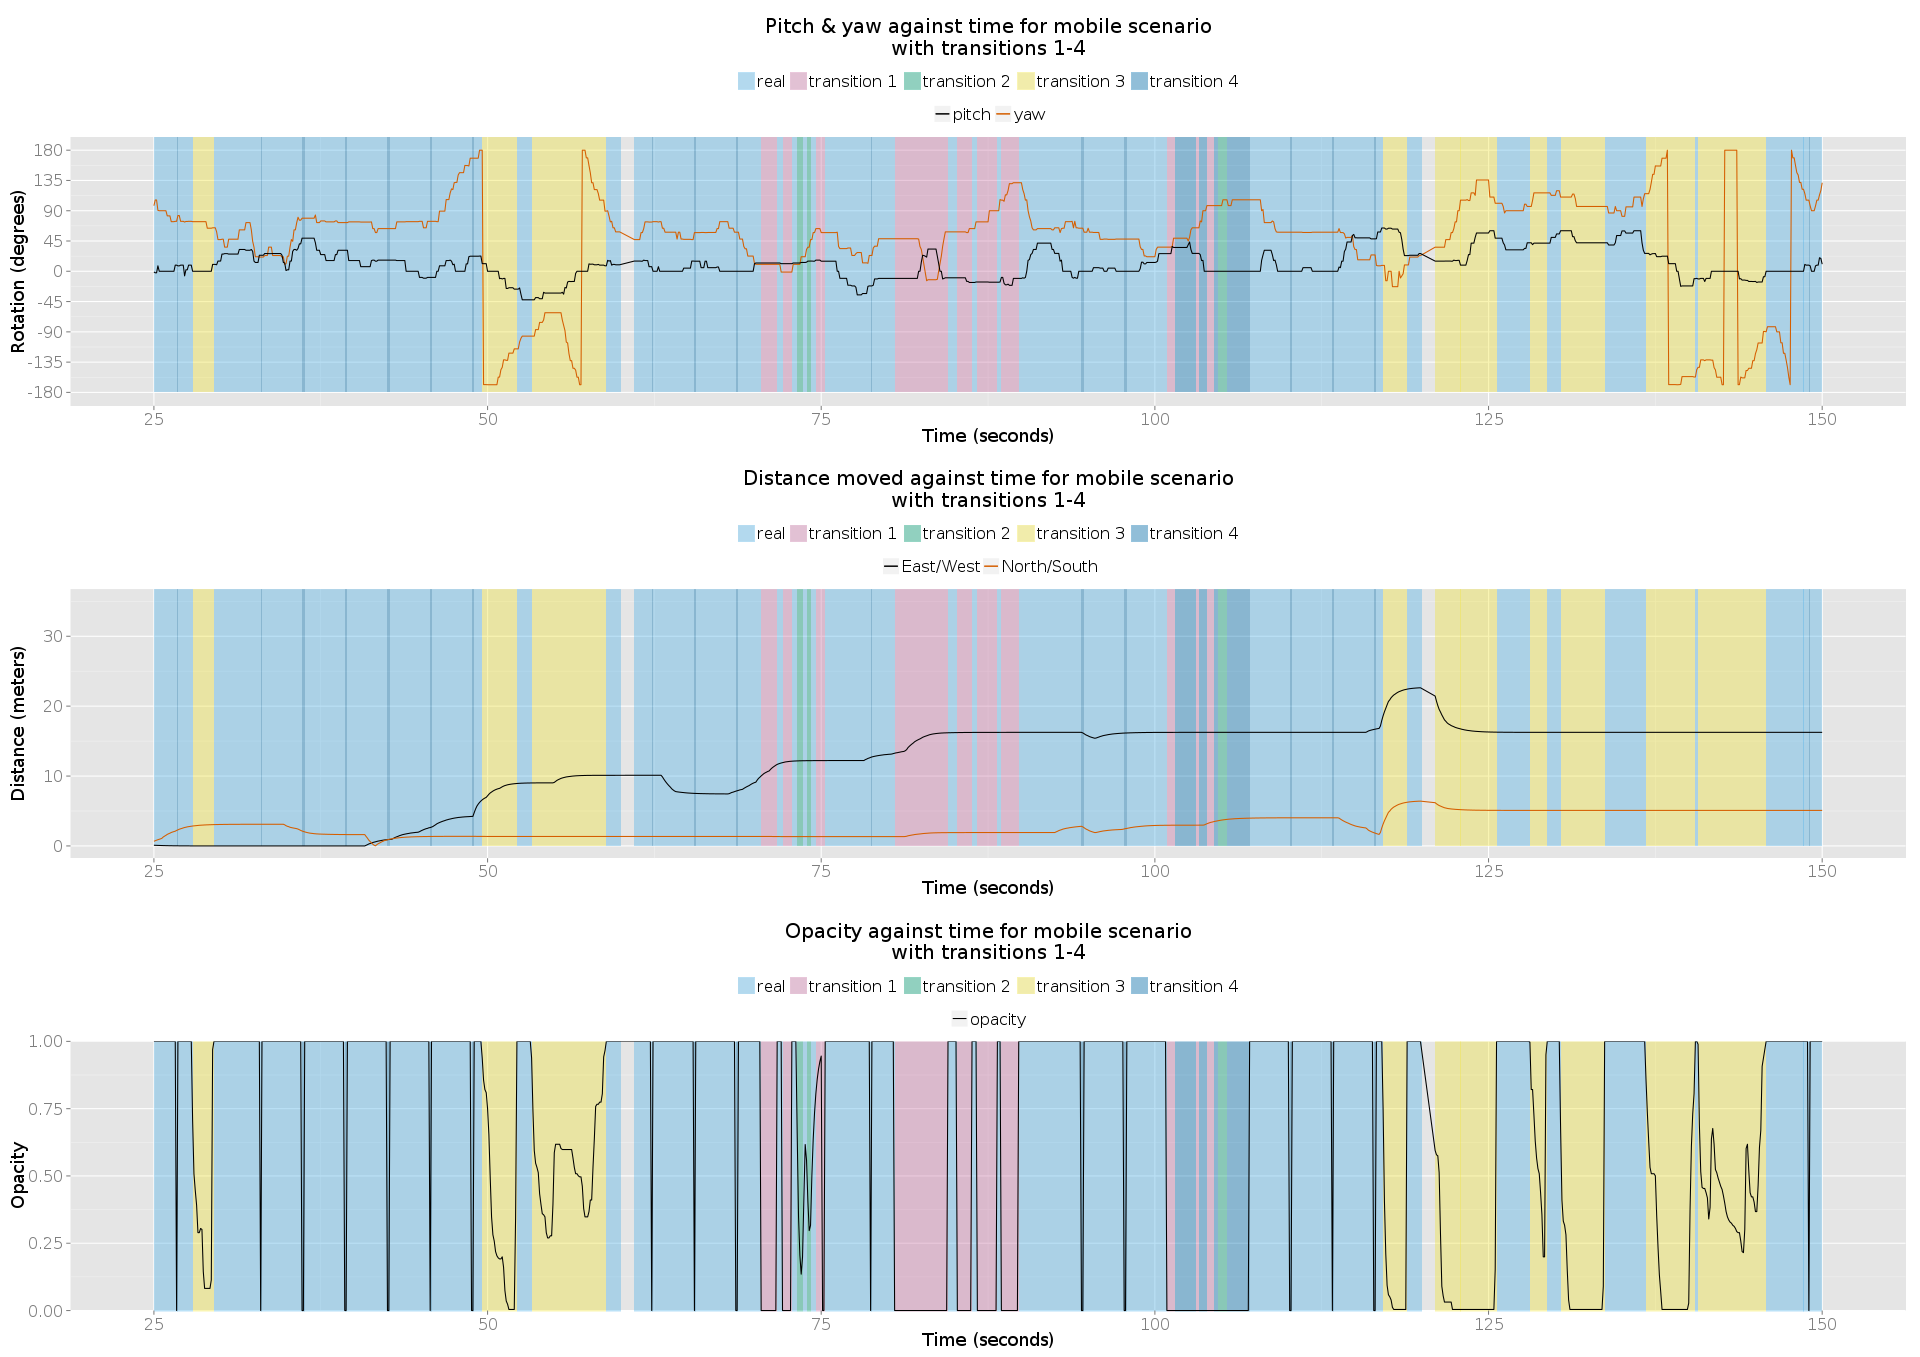
\includegraphics[width=1.2\textwidth]{2.1/12_1-4_3up.png}}
	\caption{Some images, yah.}
\end{figure}

%=========================================================================================================

\clearpage

\subsection{Participant 13}

\begin{figure}[h]
	\makebox[\textwidth][c]{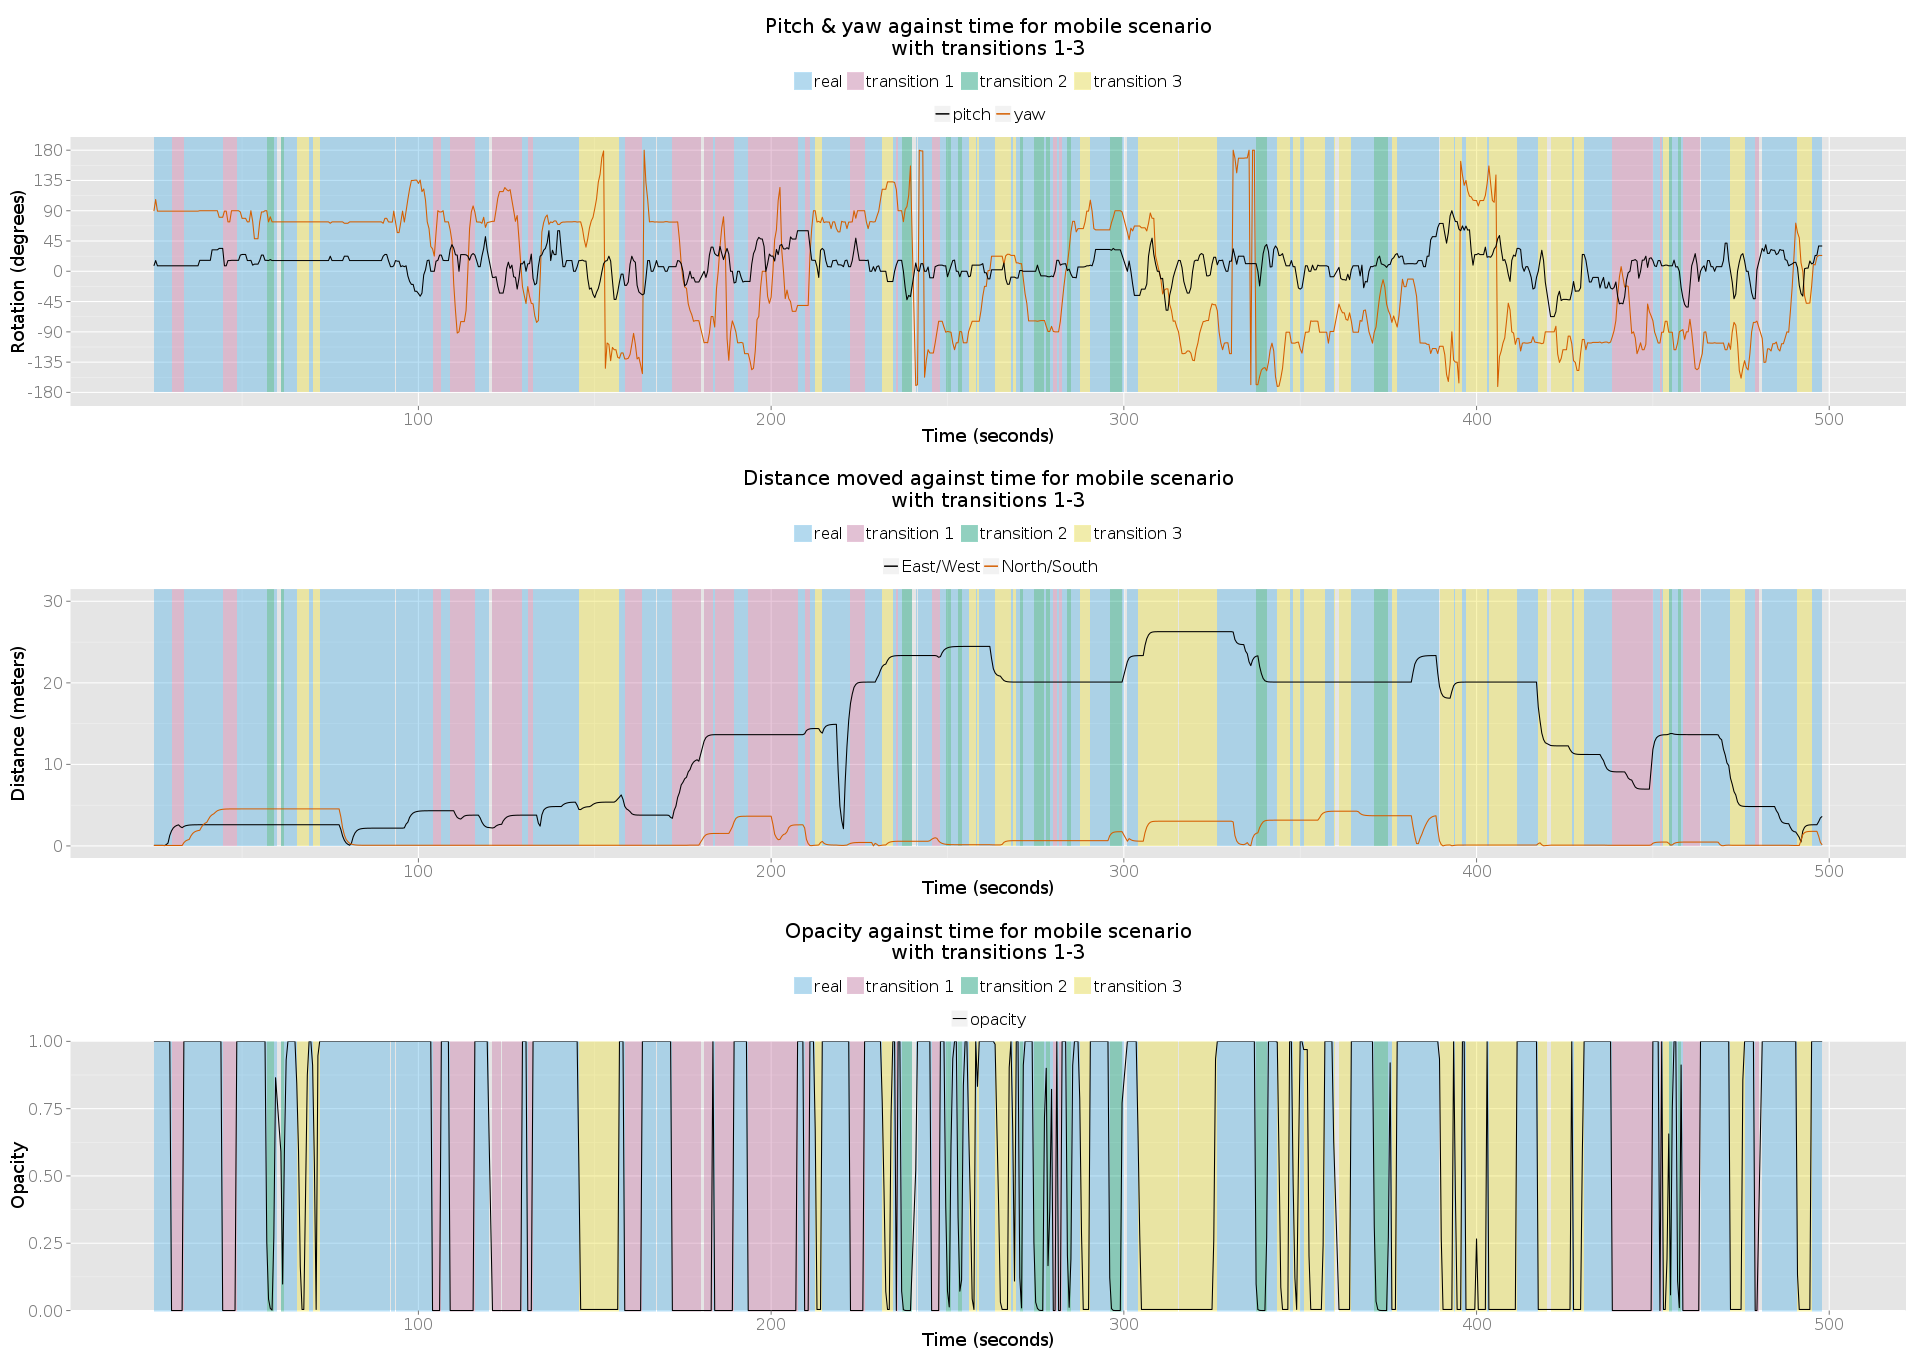
\includegraphics[width=1.2\textwidth]{2.1/13_1-3_3up.png}}
	\caption{Some images, yah.}
\end{figure}

\clearpage

\begin{figure}[h]
	\makebox[\textwidth][c]{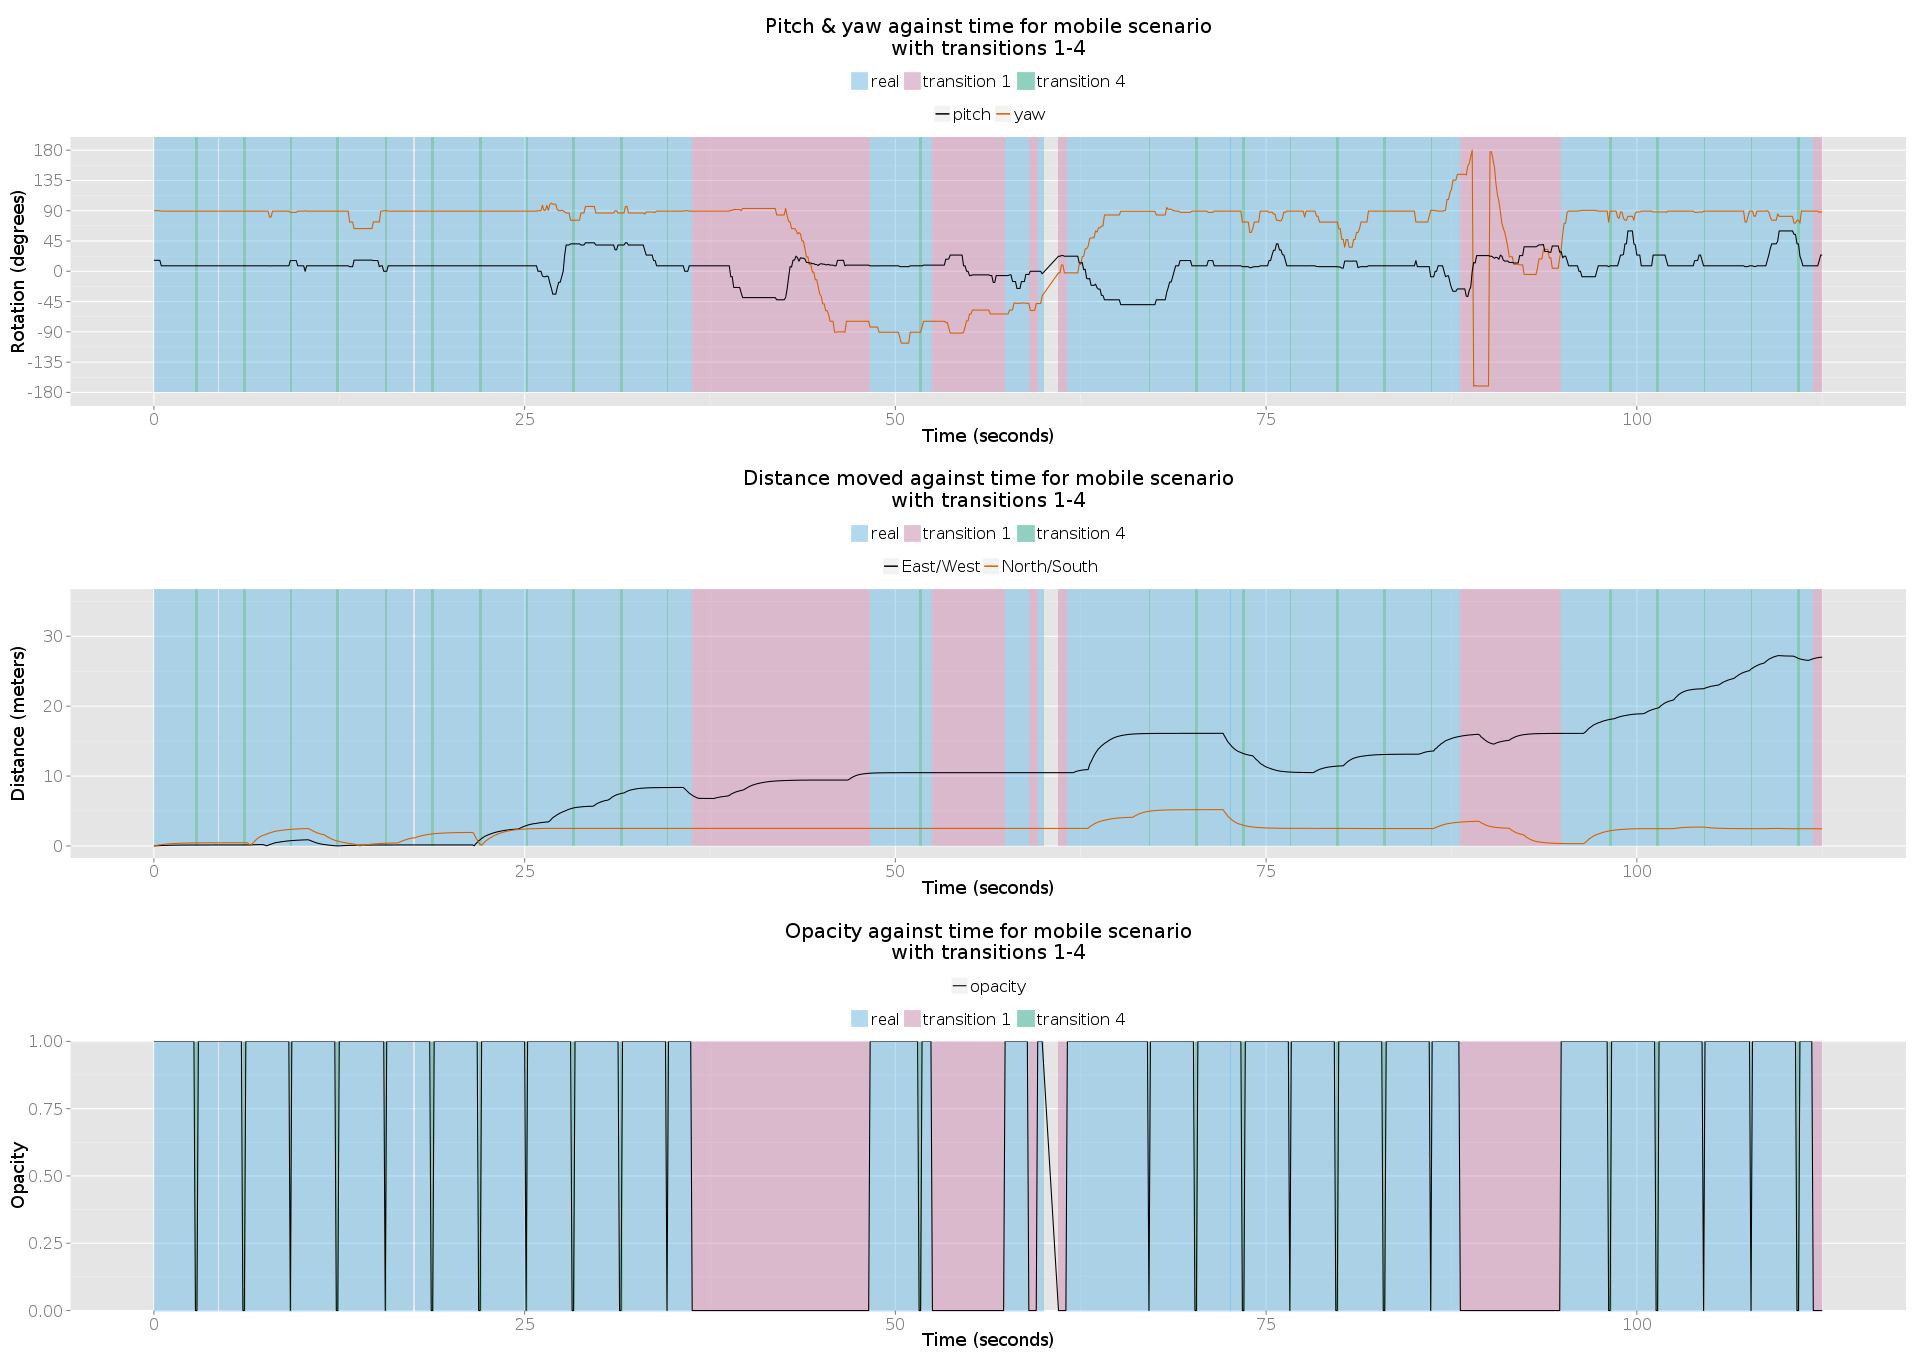
\includegraphics[width=1.2\textwidth]{2.1/13_1-4_3up.png}}
	\caption{Some images, yah.}
\end{figure}

%=========================================================================================================

\clearpage

\section{Phase 2.2 Results}

%=========================================================================================================

\clearpage

\subsection{Participant 14}

\begin{figure}[h]
	\makebox[\textwidth][c]{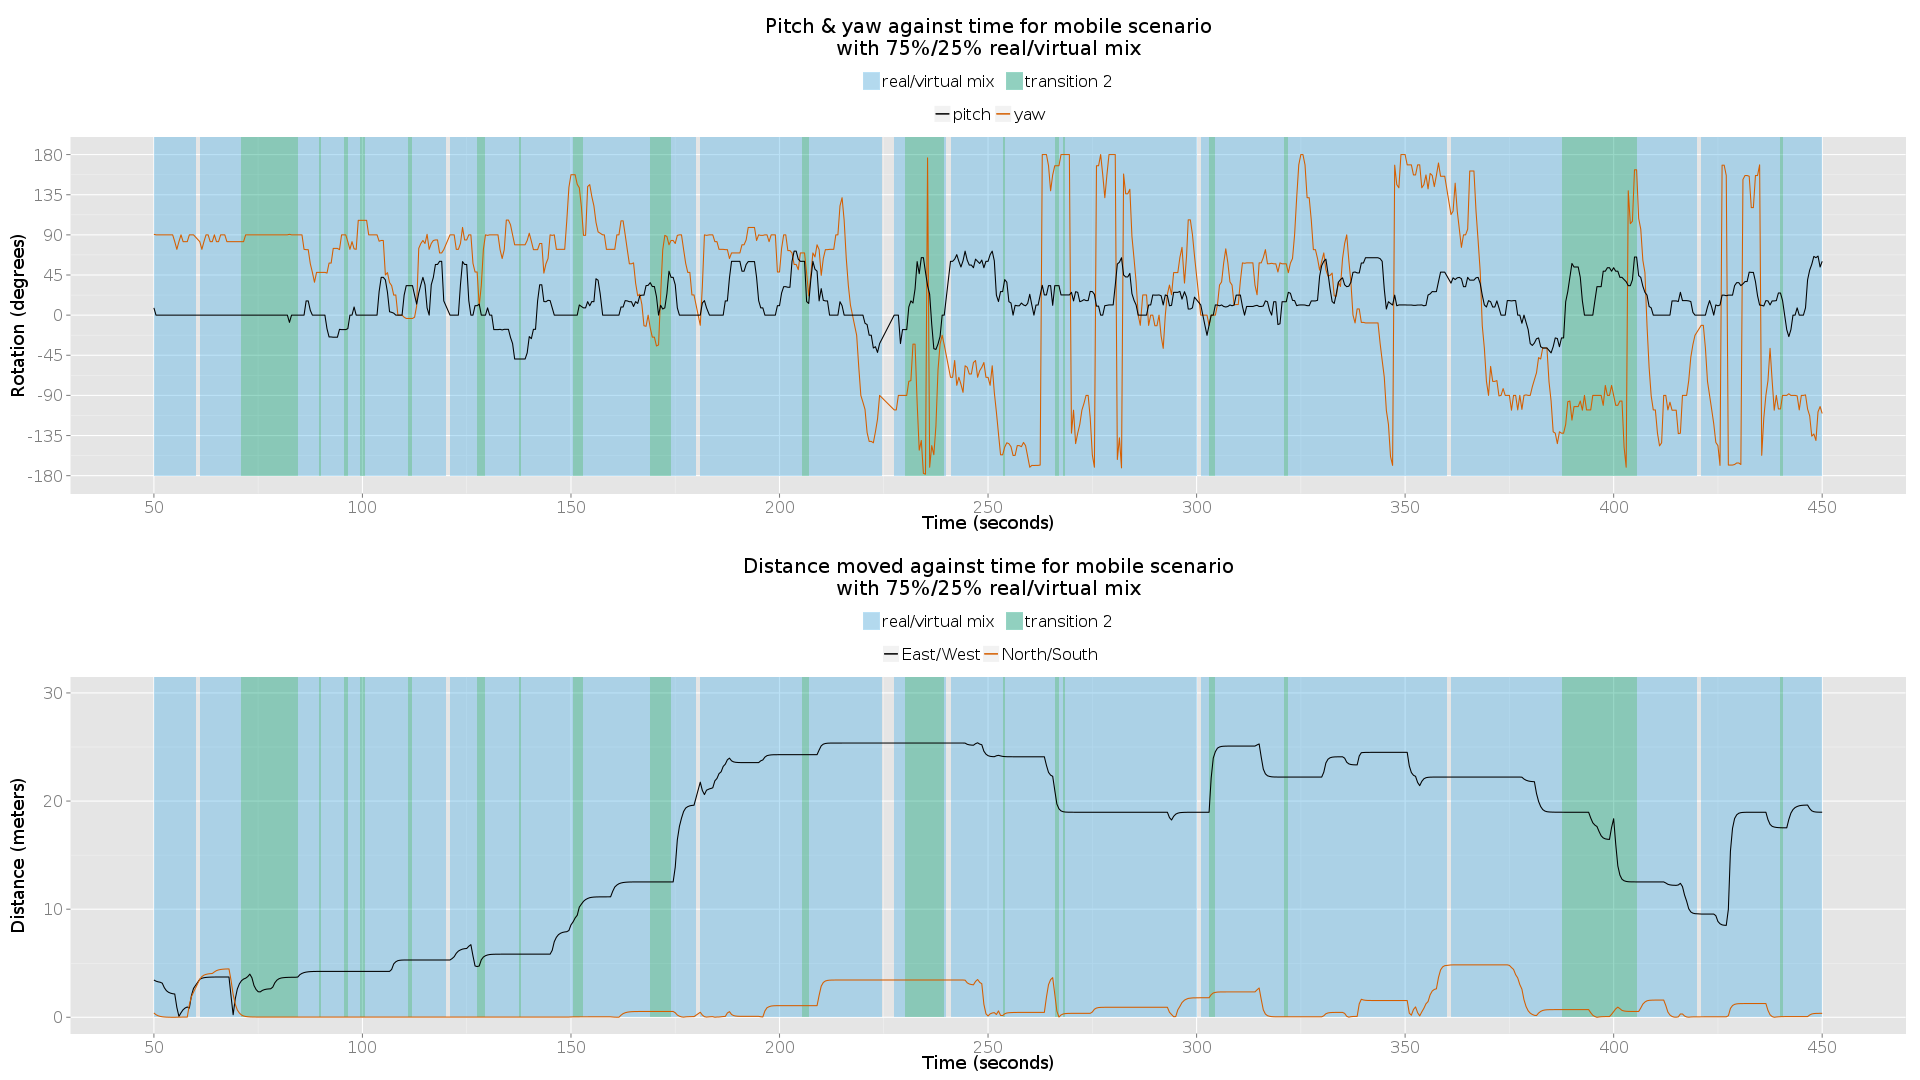
\includegraphics[width=1.2\textwidth]{2.2/14_75_2up.png}}
	\caption{Some images, yah.}
\end{figure}

\clearpage

\begin{figure}[h]
	\makebox[\textwidth][c]{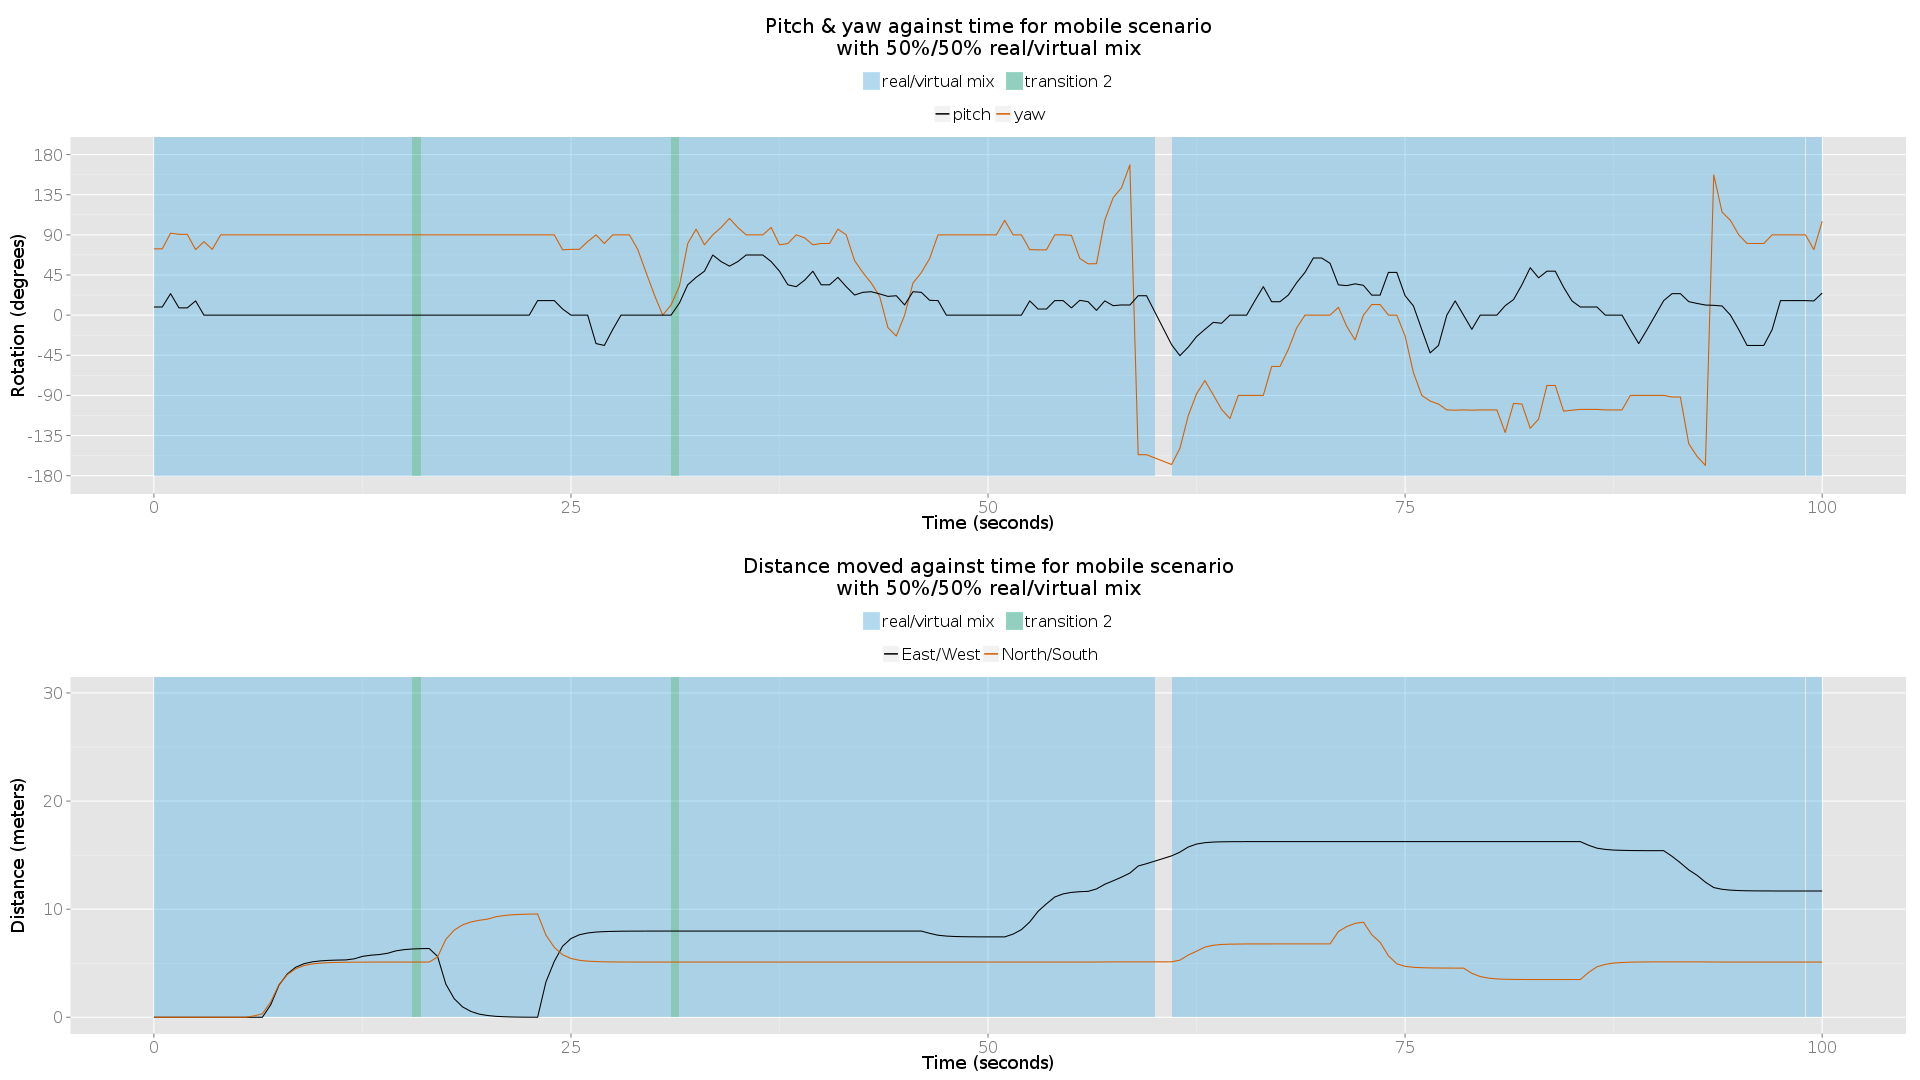
\includegraphics[width=1.2\textwidth]{2.2/14_50_2up.png}}
	\caption{Some images, yah.}
\end{figure}

%=========================================================================================================

\clearpage

\subsection{Participant 15}

\begin{figure}[h]
	\makebox[\textwidth][c]{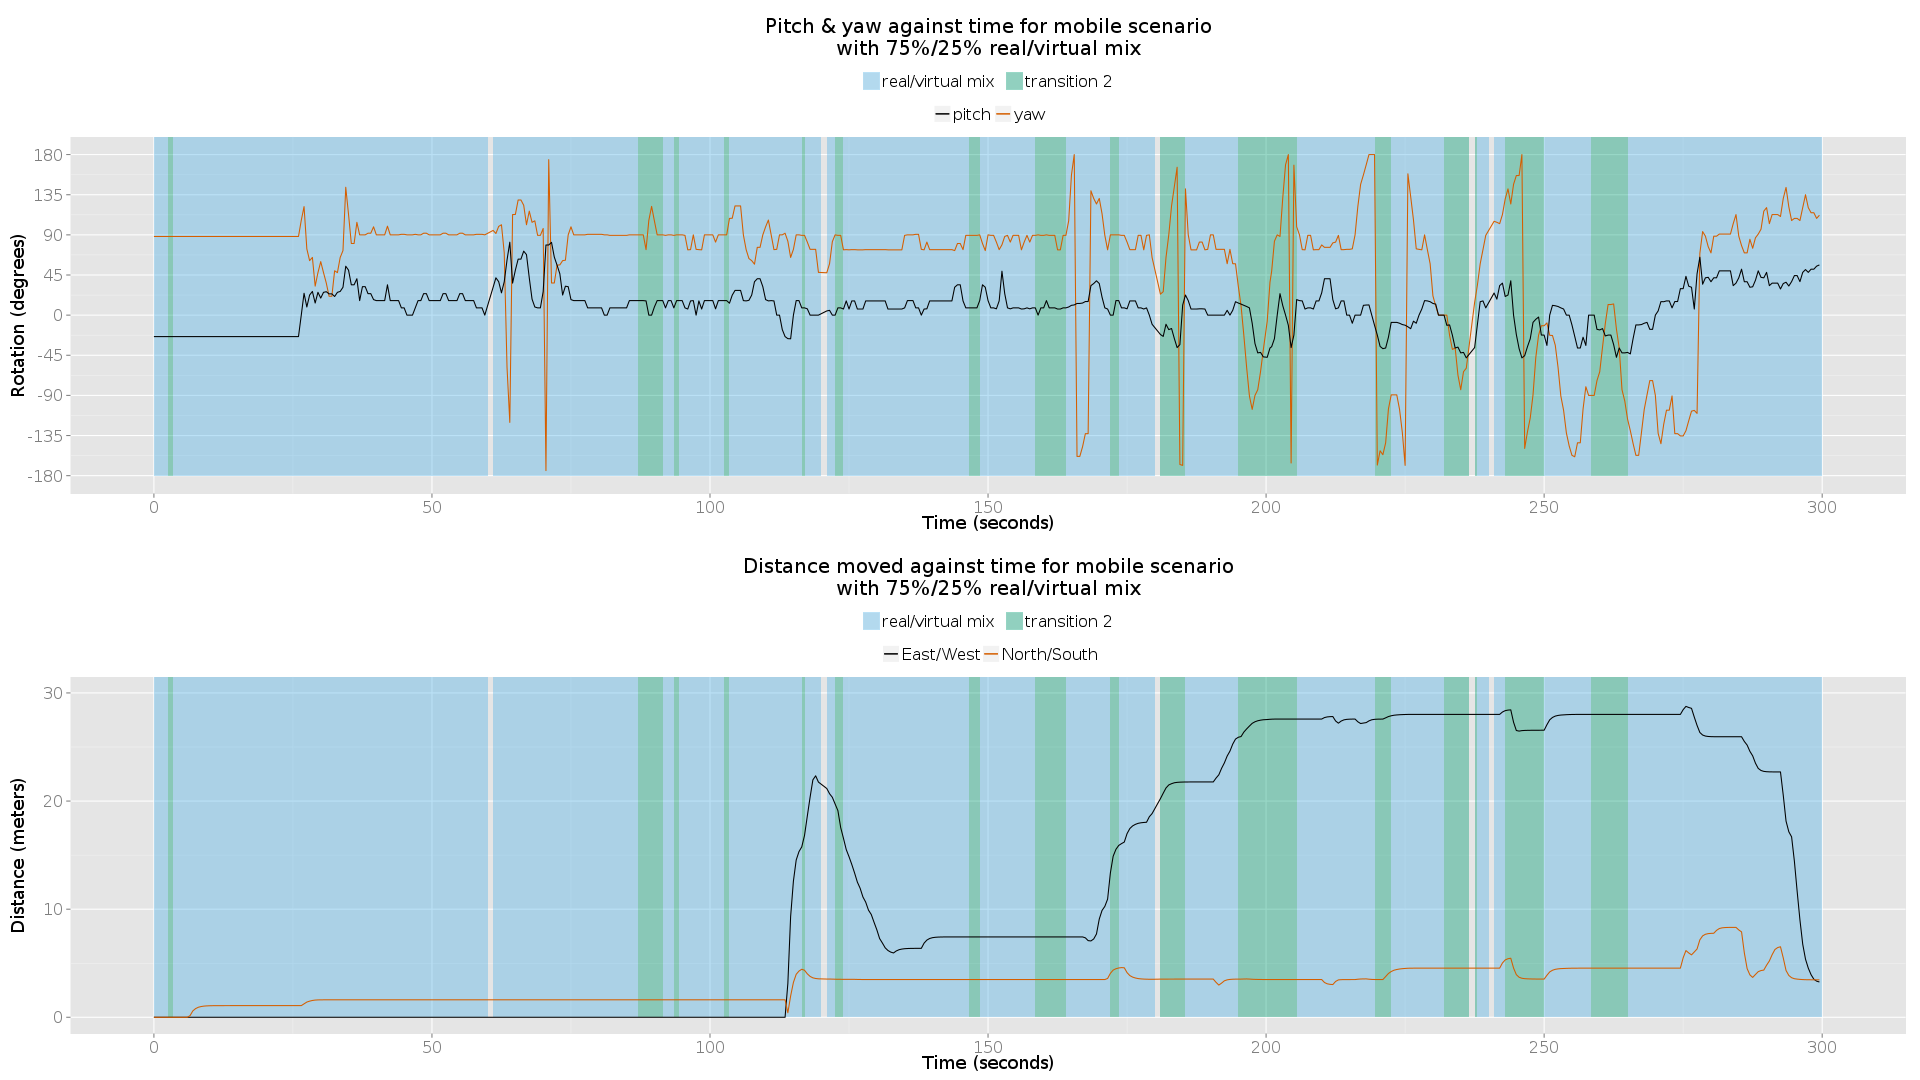
\includegraphics[width=1.2\textwidth]{2.2/15_75_2up.png}}
	\caption{Some images, yah.}
\end{figure}

\clearpage

\begin{figure}[h]
	\makebox[\textwidth][c]{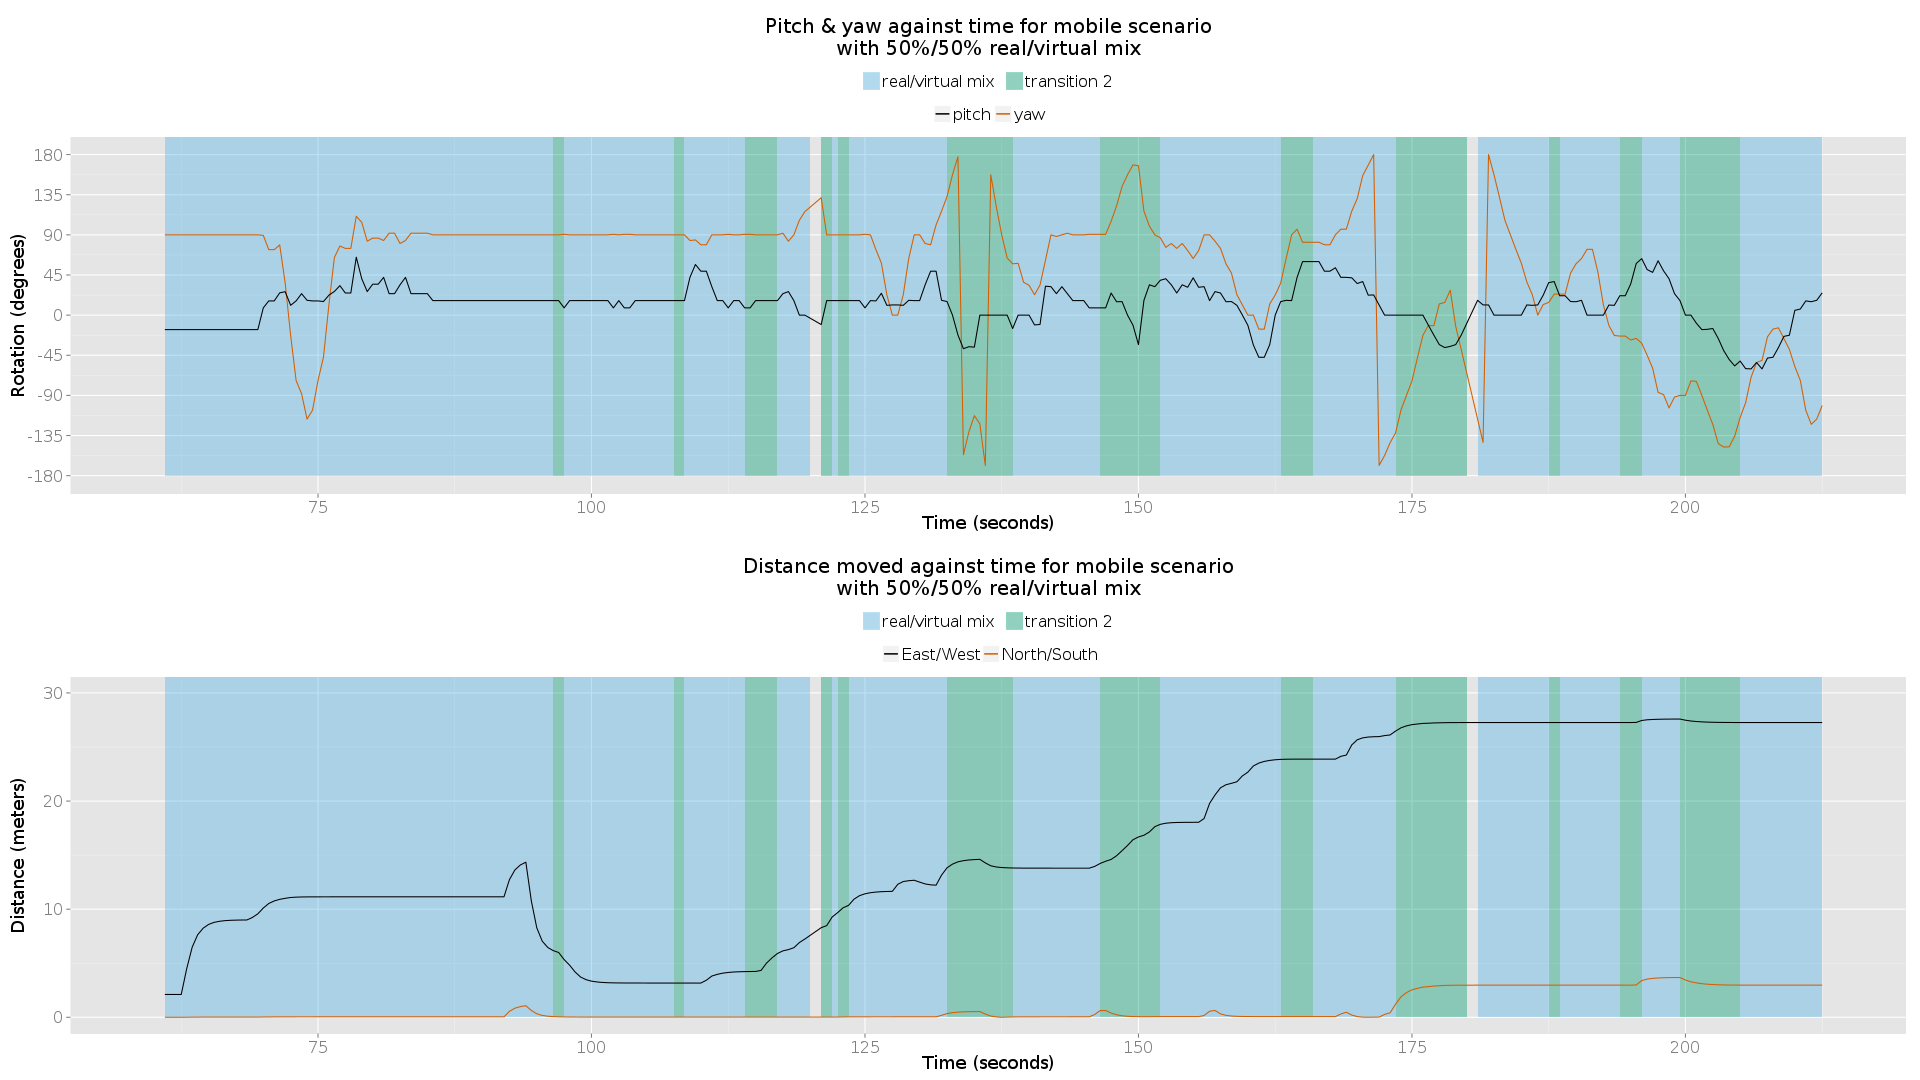
\includegraphics[width=1.2\textwidth]{2.2/15_50_2up.png}}
	\caption{Some images, yah.}
\end{figure}

%=========================================================================================================

\clearpage

\subsection{Participant 16}

\begin{figure}[h]
	\makebox[\textwidth][c]{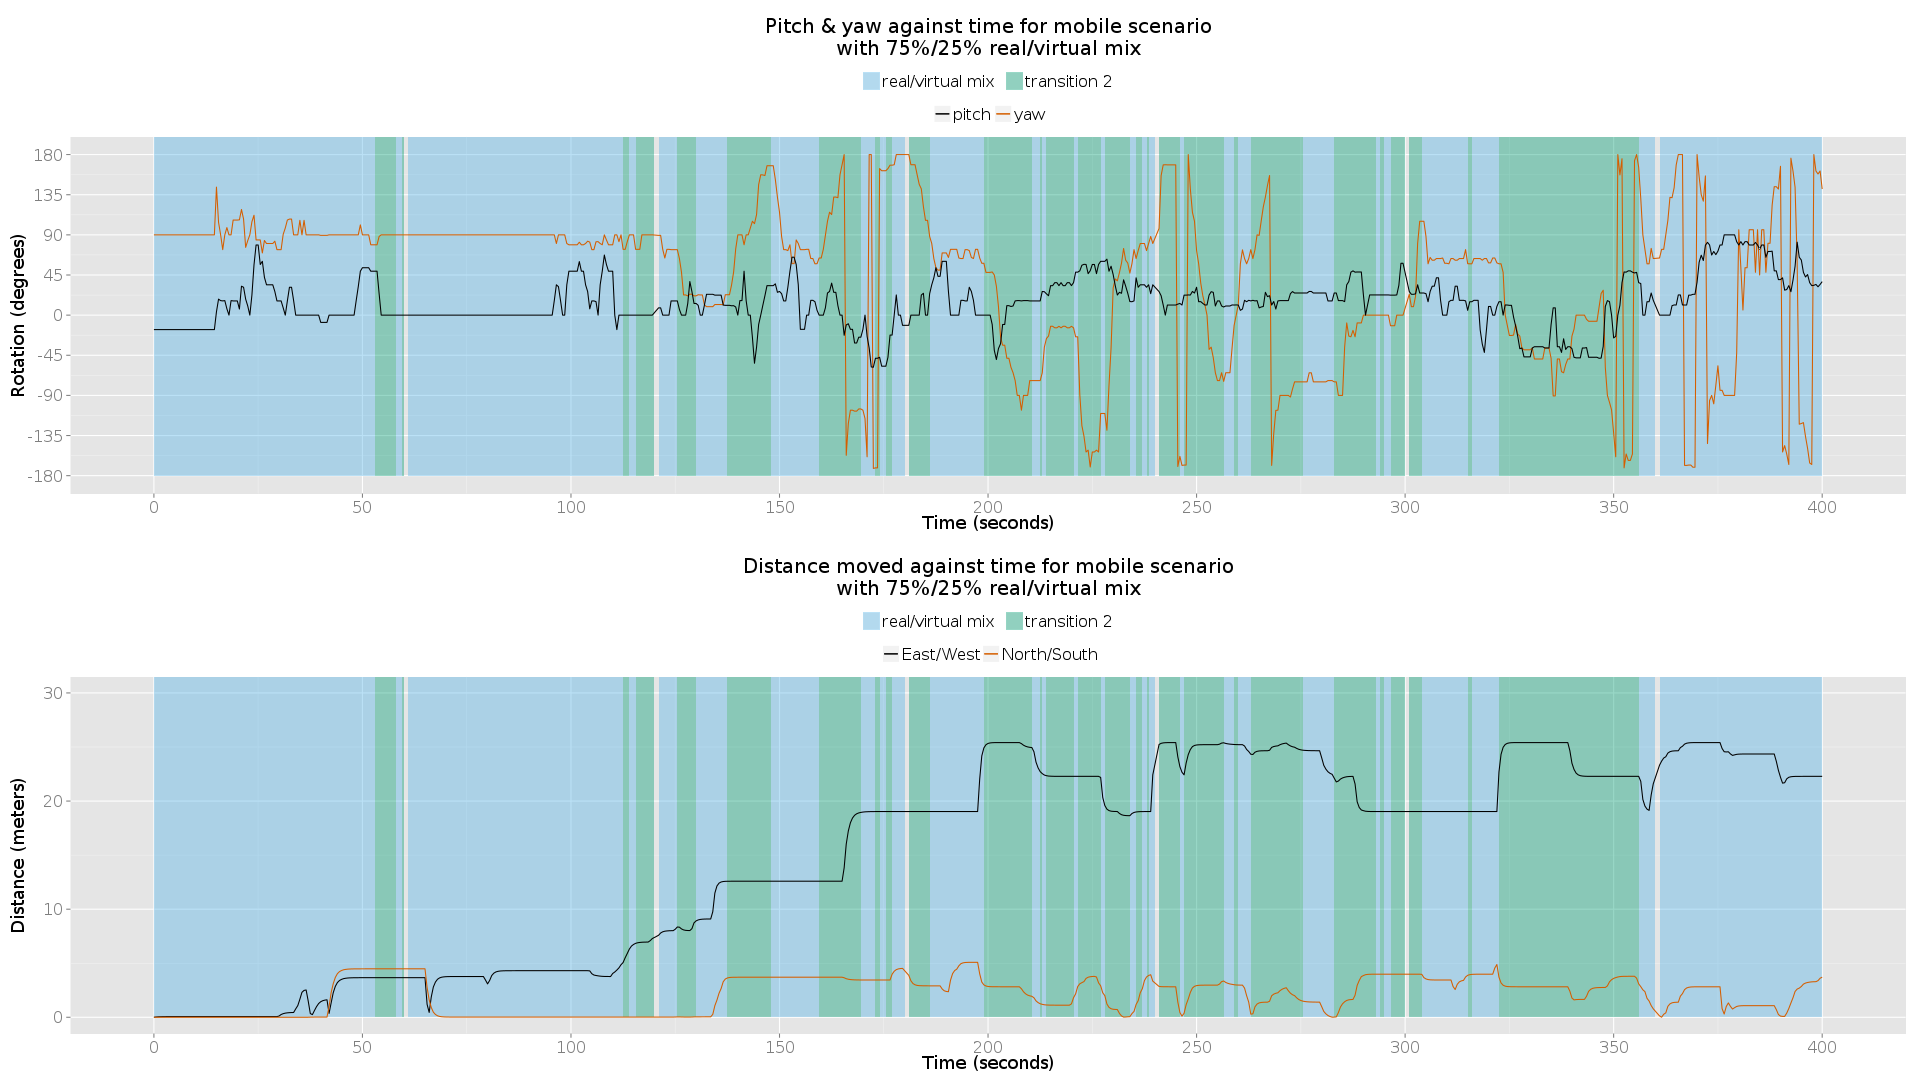
\includegraphics[width=1.2\textwidth]{2.2/16_75_2up.png}}
	\caption{Some images, yah.}
\end{figure}

\clearpage

\begin{figure}[h]
	\makebox[\textwidth][c]{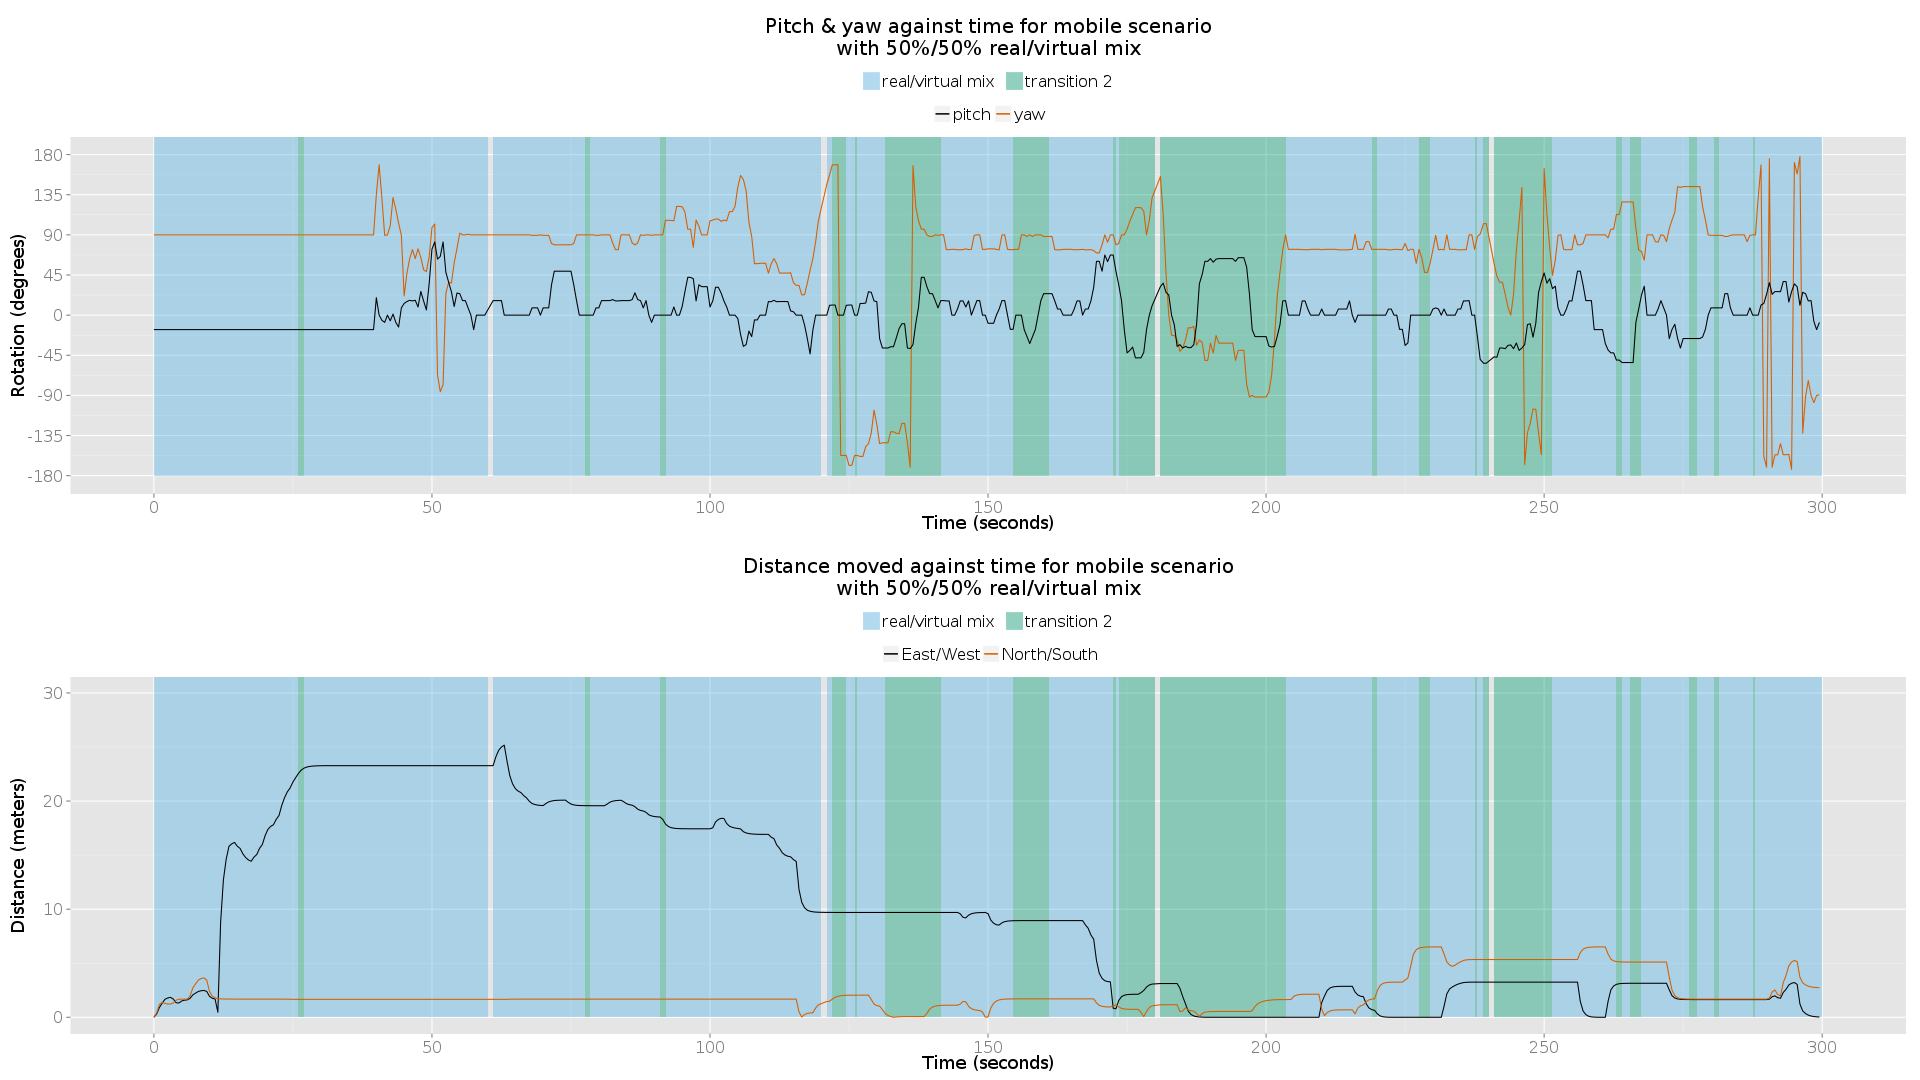
\includegraphics[width=1.2\textwidth]{2.2/16_50_2up.png}}
	\caption{Some images, yah.}
\end{figure}

%=========================================================================================================

\clearpage

\subsection{Participant 17}

\begin{figure}[h]
	\makebox[\textwidth][c]{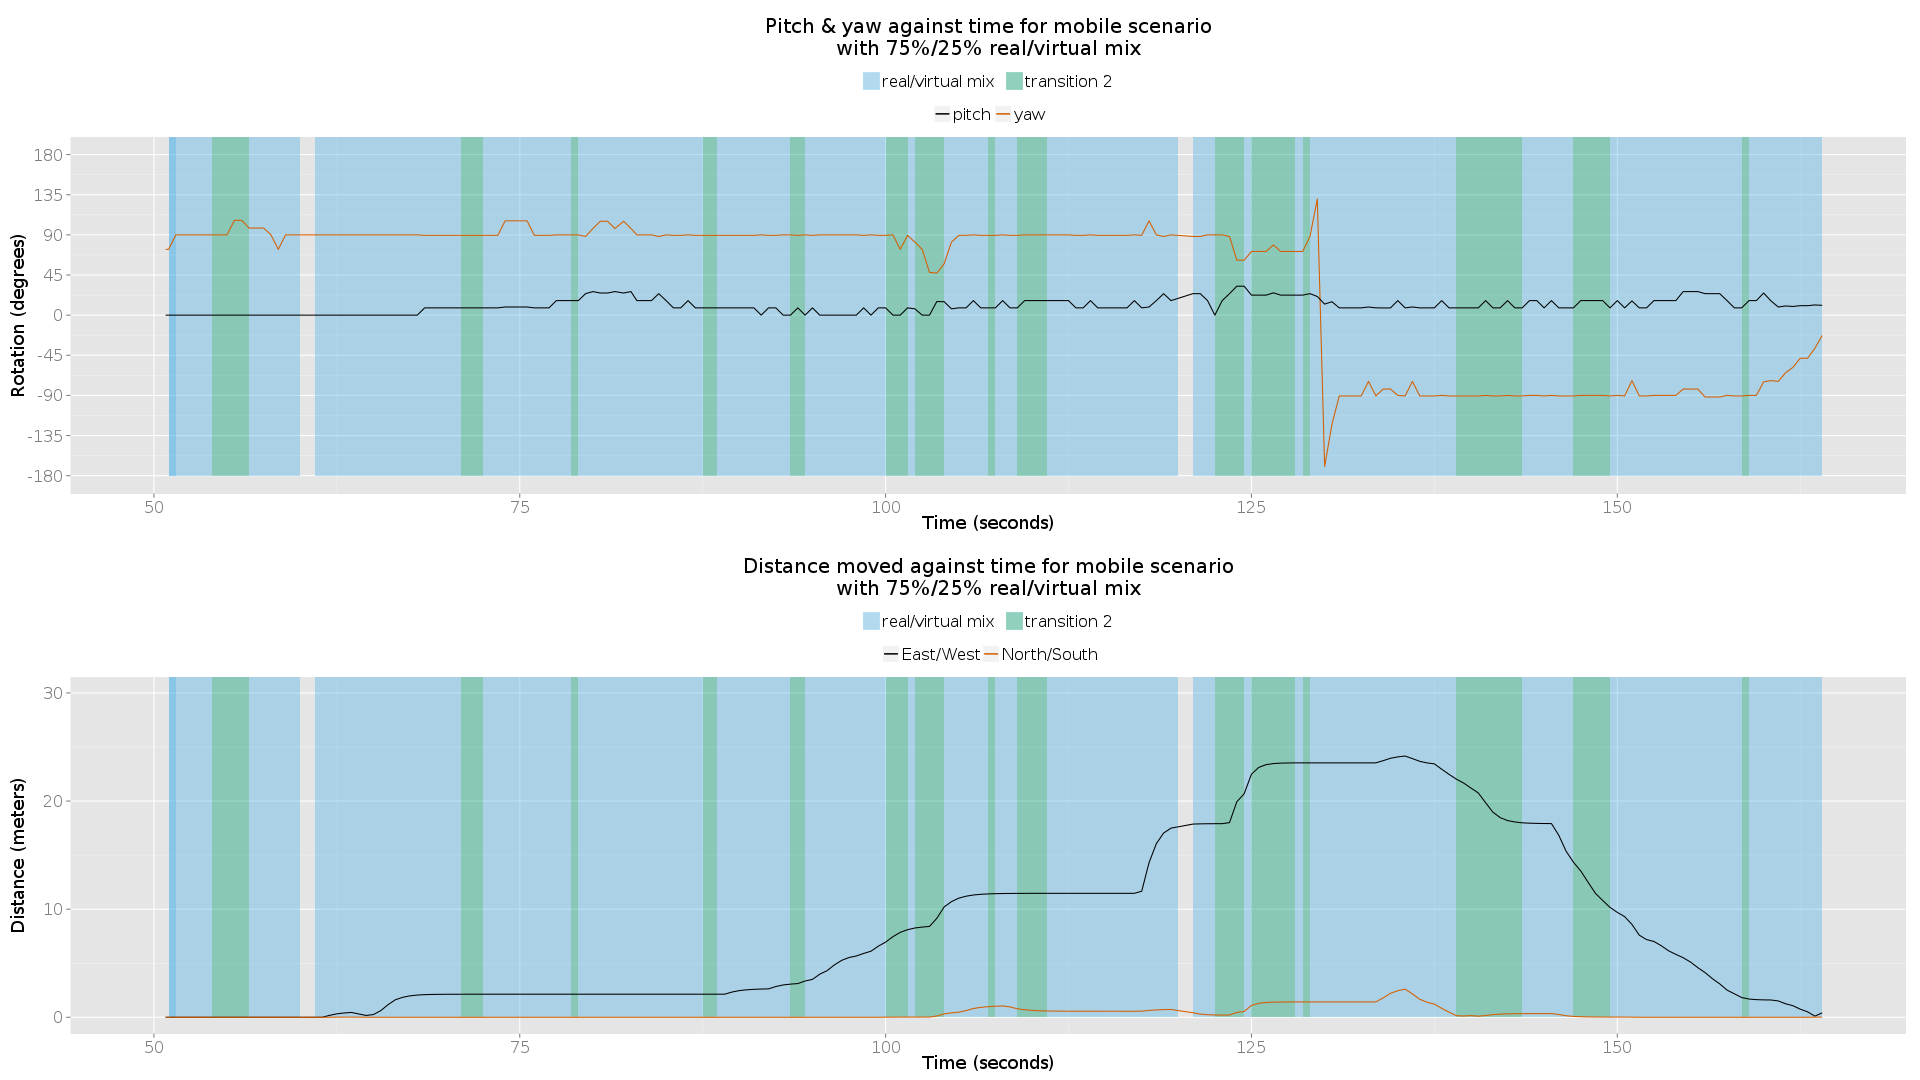
\includegraphics[width=1.2\textwidth]{2.2/17_75_2up.png}}
	\caption{Some images, yah.}
\end{figure}

\clearpage

\begin{figure}[h]
	\makebox[\textwidth][c]{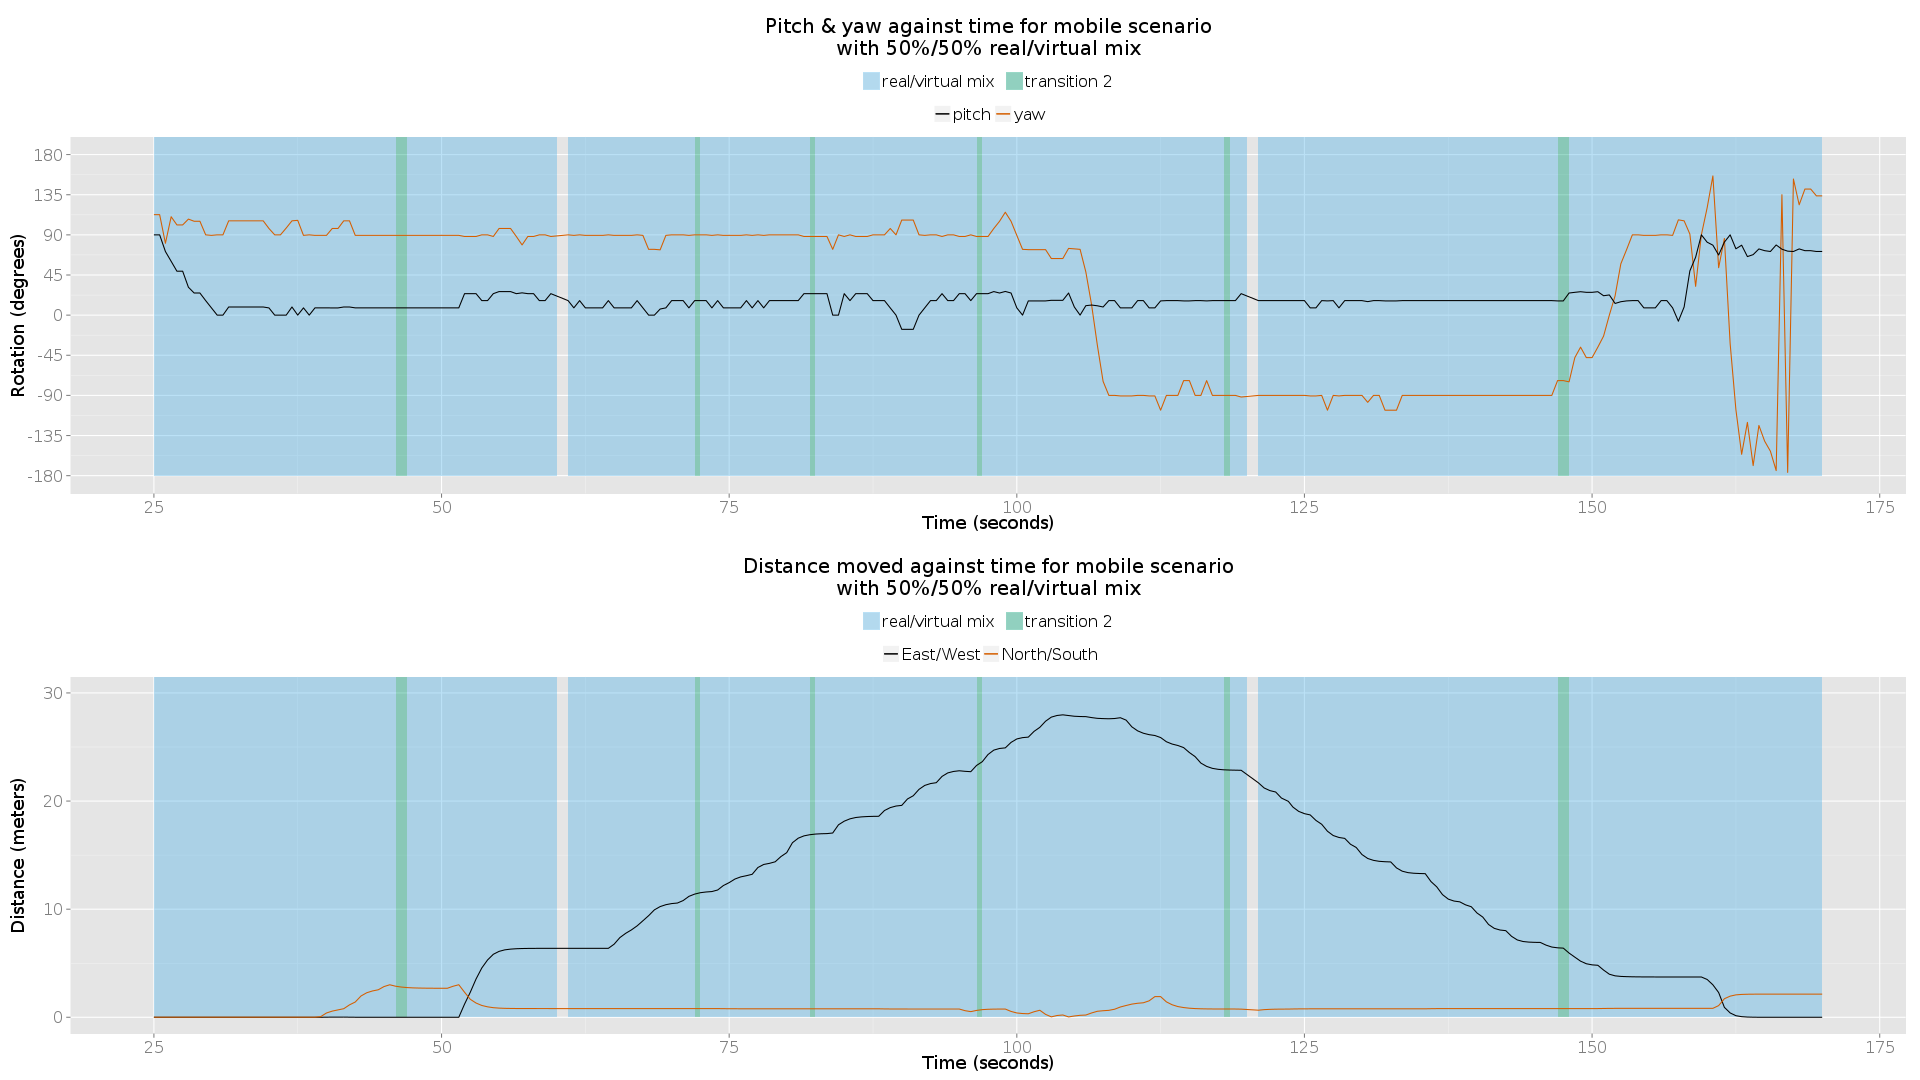
\includegraphics[width=1.2\textwidth]{2.2/17_50_2up.png}}
	\caption{Some images, yah.}
\end{figure}

%=========================================================================================================